% -*- Mode:TeX -*-

%% IMPORTANT: The official thesis specifications are available at:
%%            http://libraries.mit.edu/archives/thesis-specs/
%%
%%            Please verify your thesis' formatting and copyright
%%            assignment before submission. If you notice any
%%            discrepancies between these templates and the 
%%            MIT Libraries' specs, please let us know
%%            by e-mailing thesis@mit.edu

%% The documentclass options along with the pagestyle can be used to generate
%% a technical report, a draft copy, or a regular thesis. You may need to
%% re-specify the pagestyle after you \include cover.tex. For more
%% information, see the first few lines of mitthesis.cls. 

%\documentclass[12pt,vi,twoside]{mitthesis}
%%
%%  If you want your thesis copyright to you instead of MIT, use the
%%  ``vi'' option, as above.
%%
%\documentclass[12pt,twoside,leftblank]{mitthesis}
%%
%% If you want blank pages before new chapters to be labelled ``This
%% Page Intentionally Left Blank'', use the ``leftblank'' option, as
%% above. 

\documentclass[12pt,twoside]{misc/mitthesis}
\usepackage{misc/lgrind}
%% These have been added at the request of the MIT Libraries, because
%% some PDF conversions mess up the ligatures.  -LB, 1/22/2014
\usepackage{cmap}
\usepackage[T1]{fontenc}

% CUSTOM IMPORT PACKAGES
\usepackage{multicol}
\usepackage{graphicx}
\usepackage{listings}
\usepackage{amsfonts}
\usepackage{amsmath}
\usepackage{amssymb}

\usepackage[ruled]{algorithm2e}
\usepackage[ruled]{algorithm}
\usepackage{algorithmic}


\usepackage{blindtext}
\usepackage{hyperref}

\usepackage[table]{xcolor}
\usepackage{float}

\usepackage{cite}
\usepackage{makecell}

\usepackage{caption}
\usepackage{subcaption}
 
\usepackage{tikz}
\usetikzlibrary{shapes, arrows, positioning}
\tikzset{
  neuron missing/.style={
    scale=4,
    execute at begin node=\color{black}$...$
  }
}

% \usepackage{color, colortbl}
% \definecolor{light_gray}{rgb}{0.83, 0.83, 0.83}

% \usepackage{amsthm}
\usepackage[english]{babel}
\newtheorem{theorem}{Theorem}

\usepackage{CJKutf8}


\pagestyle{plain}

\definecolor{dkgreen}{rgb}{0,0.6,0}
\definecolor{dkblue}{rgb}{.2,.2,1}
\definecolor{gray}{rgb}{0.5,0.5,0.5}
\definecolor{mauve}{rgb}{0.58,0,0.82}

\lstset{
  language=Matlab,
  breaklines=true,
  aboveskip=1pc,
  belowskip=1pc,
  basicstyle={\linespread{0.1}\footnotesize\ttfamily},
  numbers=left,
  showstringspaces=false,
  numberstyle={\tiny\color{gray}\ttfamily},
  keywordstyle={\color{dkblue}\ttfamily},
  commentstyle={\color{dkgreen}\ttfamily},
  stringstyle={\color{mauve}\ttfamily},
}

%% This bit allows you to either specify only the files which you wish to
%% process, or `all' to process all files which you \include.
%% Krishna Sethuraman (1990).

%\typein [\files]{Enter file names to process, (chap1,chap2 ...), or `all' to process all files:}
\def\all{all}
\ifx\files\all \typeout{Including all files.} \else %\typeout{Including only \files.} \includeonly{\files} \fi

\begin{document}
% -*-latex-*-
% 
% For questions, comments, concerns or complaints:
% thesis@mit.edu
% 
%
% $Log: cover.tex,v $
% Revision 1.9  2019/08/06 14:18:15  cmalin
% Replaced sample content with non-specific text.
%
% Revision 1.8  2008/05/13 15:02:15  jdreed
% Degree month is June, not May.  Added note about prevdegrees.
% Arthur Smith's title updated
%
% Revision 1.7  2001/02/08 18:53:16  boojum
% changed some \newpages to \cleardoublepages
%
% Revision 1.6  1999/10/21 14:49:31  boojum
% changed comment referring to documentstyle
%
% Revision 1.5  1999/10/21 14:39:04  boojum
% *** empty log message ***
%
% Revision 1.4  1997/04/18  17:54:10  othomas
% added page numbers on abstract and cover, and made 1 abstract
% page the default rather than 2.  (anne hunter tells me this
% is the new institute standard.)
%
% Revision 1.4  1997/04/18  17:54:10  othomas
% added page numbers on abstract and cover, and made 1 abstract
% page the default rather than 2.  (anne hunter tells me this
% is the new institute standard.)
%
% Revision 1.3  93/05/17  17:06:29  starflt
% Added acknowledgements section (suggested by tompalka)
% 
% Revision 1.2  92/04/22  13:13:13  epeisach
% Fixes for 1991 course 6 requirements
% Phrase "and to grant others the right to do so" has been added to 
% permission clause
% Second copy of abstract is not counted as separate pages so numbering works
% out
% 
% Revision 1.1  92/04/22  13:08:20  epeisach

% NOTE:
% These templates make an effort to conform to the MIT Thesis specifications,
% however the specifications can change. We recommend that you verify the
% layout of your title page with your thesis advisor and/or the MIT 
% Libraries before printing your final copy.
\title{A Data-Driven Approach to System Dynamics Modeling and Control Design}

\author{George C. Chen}
% If you wish to list your previous degrees on the cover page, use the 
% previous degrees command:
\prevdegrees{B.S., Massachusetts Institute of Technology (2021)}
% You can use the \\ command to list multiple previous degrees
%       \prevdegrees{B.S., University of California (1978) \\
%                    S.M., Massachusetts Institute of Technology (1981)}
\department{Department of Mechanical Engineering}

% If the thesis is for two degrees simultaneously, list them both
% separated by \and like this:
% \degree{Doctor of Philosophy \and Master of Science}
\degree{Master of Science in Mechanical Engineering}

% As of the 2007-08 academic year, valid degree months are September, 
% February, or June.  The default is June.
\degreemonth{May}
\degreeyear{2022}
\thesisdate{May 6, 2022}

%% By default, the thesis will be copyrighted to MIT.  If you need to copyright
%% the thesis to yourself, just specify the `vi' documentclass option.  If for
%% some reason you want to exactly specify the copyright notice text, you can
%% use the \copyrightnoticetext command.  
%\copyrightnoticetext{\copyright IBM, 1990.  Do not open till Xmas.}

% If there is more than one supervisor, use the \supervisor command
% once for each.
\supervisor{Dr. Brian W. Anthony}{Principal Research Scientist}

% This is the department committee chairman, not the thesis committee
% chairman.  You should replace this with your Department's Committee
% Chairman.
\chairman{Nicolas Hadjiconstantinou}{Graduate Officer}

% Make the titlepage based on the above information.  If you need
% something special and can't use the standard form, you can specify
% the exact text of the titlepage yourself.  Put it in a titlepage
% environment and leave blank lines where you want vertical space.
% The spaces will be adjusted to fill the entire page.  The dotted
% lines for the signatures are made with the \signature command.
\maketitle

% The abstractpage environment sets up everything on the page except
% the text itself.  The title and other header material are put at the
% top of the page, and the supervisors are listed at the bottom.  A
% new page is begun both before and after.  Of course, an abstract may
% be more than one page itself.  If you need more control over the
% format of the page, you can use the abstract environment, which puts
% the word "Abstract" at the beginning and single spaces its text.

%% You can either \input (*not* \include) your abstract file, or you can put
%% the text of the abstract directly between the \begin{abstractpage} and
%% \end{abstractpage} commands.

% First copy: start a new page, and save the page number.
\cleardoublepage
% Uncomment the next line if you do NOT want a page number on your
% abstract and acknowledgments pages.
% \pagestyle{empty}
\setcounter{savepage}{\thepage}
\begin{abstractpage}
% $Log: abstract.tex,v $
% Revision 1.1  93/05/14  14:56:25  starflt
% Initial revision
% 
% Revision 1.1  90/05/04  10:41:01  lwvanels
% Initial revision
% 
%
%% The text of your abstract and nothing else (other than comments) goes here.
%% It will be single-spaced and the rest of the text that is supposed to go on
%% the abstract page will be generated by the abstractpage environment.  This
%% file should be \input (not \include 'd) from cover.tex.


This thesis presents an in-depth investigation on modeling and simulation of an optical fiber extrusion system and its controllers in production. With measured production data during the fiber drawing process, a long short-term memory (LSTM) neural network is architected, implemented, and trained to model the process dynamics of the fiber drawing plant. Training experiments were conducted to investigate the effect of several parameters on the model’s performance. Furthermore, statistical analysis models with assumed structures are employed as part of the black-box system identification process to model controllers in the production system, subject to noise and disturbances. With aforementioned components, a closed-loop simulation of the fiber extrusion system is then developed in MATLAB, proving the feasibility of simulating mechanical systems in production using learned models. The approach developed in this study is suitable for data-driven deployment of many kinds of manufacturing plants in production, which may have limited operational domains due to mechanical constraints. The simulation, once implemented in hardware, could potentially replace the laborious, iterative tuning process of the controllers, and serve as a design tool to optimize these controllers using a digital twin.

% currently: 185 words

% NO LONGER THAN 350 WORDS! 

\end{abstractpage}

% Additional copy: start a new page, and reset the page number.  This way,
% the second copy of the abstract is not counted as separate pages.
% Uncomment the next 6 lines if you need two copies of the abstract
% page.
% \setcounter{page}{\thesavepage}
% \begin{abstractpage}
% % $Log: abstract.tex,v $
% Revision 1.1  93/05/14  14:56:25  starflt
% Initial revision
% 
% Revision 1.1  90/05/04  10:41:01  lwvanels
% Initial revision
% 
%
%% The text of your abstract and nothing else (other than comments) goes here.
%% It will be single-spaced and the rest of the text that is supposed to go on
%% the abstract page will be generated by the abstractpage environment.  This
%% file should be \input (not \include 'd) from cover.tex.


This thesis presents an in-depth investigation on modeling and simulation of an optical fiber extrusion system and its controllers in production. With measured production data during the fiber drawing process, a long short-term memory (LSTM) neural network is architected, implemented, and trained to model the process dynamics of the fiber drawing plant. Training experiments were conducted to investigate the effect of several parameters on the model’s performance. Furthermore, statistical analysis models with assumed structures are employed as part of the black-box system identification process to model controllers in the production system, subject to noise and disturbances. With aforementioned components, a closed-loop simulation of the fiber extrusion system is then developed in MATLAB, proving the feasibility of simulating mechanical systems in production using learned models. The approach developed in this study is suitable for data-driven deployment of many kinds of manufacturing plants in production, which may have limited operational domains due to mechanical constraints. The simulation, once implemented in hardware, could potentially replace the laborious, iterative tuning process of the controllers, and serve as a design tool to optimize these controllers using a digital twin.

% currently: 185 words

% NO LONGER THAN 350 WORDS! 

% \end{abstractpage}

\cleardoublepage

\section*{Acknowledgment}

Words cannot describe my gratitude for all who have supported me directly and indirectly throughout my graduate career at MIT. This thesis would not have been possible without you all. 

First and foremost, I would like to thank Dr. Brian Anthony, my thesis supervisor, for the guidance and mentorship that significantly contributed to the fruition of this thesis. I am grateful for your support of my career path forward. 

Furthermore, I am thankful for my labmate Victor Reyes, with whom I closely collaborated on this research project. Our discussions on machine learning and data analysis were immensely helpful in making forward progress in experimentation setup and analyses. I am fortunate to have collaborated with you to realize the theoretical ideas presented in this thesis. 

Last but not least, I would like to thank my parents, Yigang Chen and Yonghong Zhang. My achievements could not have been possible without your unconditional love and unwavering support for my entire lifetime. Immigrating to the US was not an easy transition; despite all the hardships that came our way, your spirit of perseverance empowered me to overcome my own hardships. You made sacrifices that created opportunities for me to achieve great heights in academia and beyond. For all you have done, I am eternally grateful.


\begin{CJK*}{UTF8}{gbsn} % gbsn / gkai
最后,诚挚感谢我的父母%陈奕港先生和张永红女士
。我今天的成就离不开您们二十余载无条件的爱与义无反顾的支持。举家移民谈何容易,重重困难中,您们目光里的坚定化为我前进路上的无限动力。感恩您们日日付出为我创造的平台,让我能在学业与事业上攀登新的高峰。乌鸟私情,愿乞终养。行文于此,以表孝心。
\end{CJK*}



%%%%%%%%%%%%%%%%%%%%%%%%%%%%%%%%%%%%%%%%%%%%%%%%%%%%%%%%%%%%%%%%%%%%%%
% -*-latex-*-

% Some departments (e.g. 5) require an additional signature page.  See
% signature.tex for more information and uncomment the following line if
% applicable.
% % -*- Mode:TeX -*-
%
% Some departments (e.g. Chemistry) require an additional cover page
% with signatures of the thesis committee.  Please check with your
% thesis advisor or other appropriate person to determine if such a 
% page is required for your thesis.  
%
% If you choose not to use the "titlepage" environment, a \newpage
% commands, and several \vspace{\fill} commands may be necessary to
% achieve the required spacing.  The \signature command is defined in
% the "mitthesis" class
%
% The following sample appears courtesy of Ben Kaduk <kaduk@mit.edu> and
% was used in his June 2012 doctoral thesis in Chemistry. 

\begin{titlepage}
\begin{large}
This doctoral thesis has been examined by a Committee of the Department
of Chemistry as follows:

\signature{Professor Jianshu Cao}{Chairman, Thesis Committee \\
   Professor of Chemistry}

\signature{Professor Troy Van Voorhis}{Thesis Supervisor \\
   Associate Professor of Chemistry}

\signature{Professor Robert W. Field}{Member, Thesis Committee \\
   Haslam and Dewey Professor of Chemistry}
\end{large}
\end{titlepage}


\pagestyle{plain}
% \begin{center}
%     \chapter*{Dedication}
%     For idk yet\\
%     make font bigger \\
%     \begin{CJK*}{UTF8}{gbsn} % or gkai
%     写上中文,换个字体
%     \end{CJK*}
% \end{center}
  % -*- Mode:TeX -*-
%% This file simply contains the commands that actually generate the table of
%% contents and lists of figures and tables.  You can omit any or all of
%% these files by simply taking out the appropriate command.  For more
%% information on these files, see appendix C.3.3 of the LaTeX manual. 
\tableofcontents
\newpage
\listoffigures
\newpage
\listoftables


%% This is an example first chapter.  You should put chapter/appendix that you
%% write into a separate file, and add a line \include{yourfilename} to
%% main.tex, where `yourfilename.tex' is the name of the chapter/appendix file.
%% You can process specific files by typing their names in at the 
%% \files=
%% prompt when you run the file main.tex through LaTeX.

% This is an example of how you would use tgrind to include an example
% of source code; it is commented out in this template since the code
% example file does not exist. To use it, you need to remove the '%' on the
% beginning of the line, and insert your own information in the call.
%
% \tagrind[htbp]{code/pmn.s.tex}{Code sample}{opt:pmn}


\chapter{Introduction} \label{ch:intro}

\section{Motivation} \label{ch:intro:motiv}

The fiber extrusion technology is known to have profound impact on the development of energy storage devices, synthetic polymers, wearable electronics, and many more \cite{synthetic, wearable_energy1, wearable_energy2}. Especially, optical fiber manufacturing has been an integral part of high-speed communication technology. In partnership with Sterlite Technologies Ltd. (hereinafter referred to as Sterlite), MIT's Device Realization Lab is innovating new approaches to improve the optical fiber extrusion process, specifically the controller design, simulation, tuning, and deployment process. A typical fiber draw tower in production is shown in Figure \ref{fig:tower}. 

\begin{figure}[hb!]
    \centering
    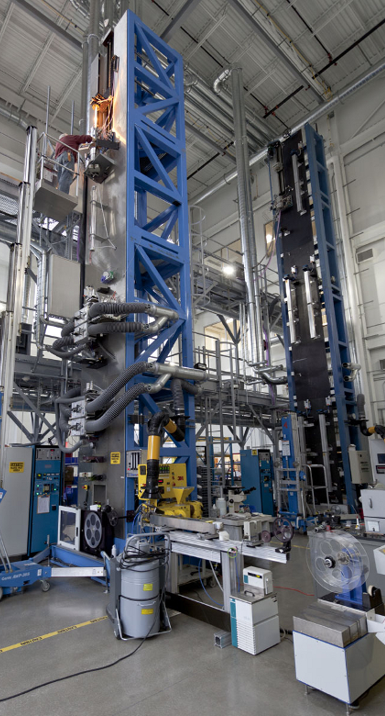
\includegraphics[width=0.5\textwidth]{figures/tower.png}
    \caption{Industrial optical fiber drawing tower on the production floor.}
    \label{fig:tower}
\end{figure}

There are many challenges in deploying new controllers to established, industrial-grade equipment. One of the challenges is to choose an appropriate method to develop an adequate model to explain the inner workings of the aggregate processes and controllers. There are three methods by which such models are created, 
\begin{enumerate}
    \item \textbf{White-box models}, which necessitate complete insight into the underlying physics to develop a model; 
    \item \textbf{Black-box models}, which require no knowledge of the internal structure and are developed solely on input-output data;
    \item \textbf{Grey-box models}, which are hybrids of the two approaches above, combining measured data and partially represented physics.
\end{enumerate}

Another challenge resides in tuning multiple controllers while obeying their limited operational design domain. Conventionally, controller tuning in the production plant is done in an isolated, trial-and-error fashion – make a small tweak to one of the parameters, examine the output, rely on intuition to consider the next tuning parameter, and repeat until performance is satisfied. The disadvantage of this approach is apparent; aside from the time- and labor- intensiveness of the process, mechanical systems often have practical constraints for safety measures (e.g. actuator limits, ramp rate, etc), which prevent the system from receiving any arbitrary control input \cite{constraints}. Using this approach, in order to simultaneously develop multiple controllers to achieve production quality, system integration may require multiple design and debugging iterations. Such modifications often lead to unnecessary downtime in production and monetary costs in research and development. 

This research project presents a data-driven approach to model nonlinear system dynamics and highlights the implementation in active optical fiber manufacturing processes, for which limited experimentation is possible. The need for better controllers is driven by the goals of reduced production variation and quicker recovery from production defects. A procedure to verify product performance and deploy systems to production is also provided as a recommendation. 

\section{Optical Fiber Extrusion Process}\label{ch:intro:fiber}

\begin{figure}[ht!]
    \centering
    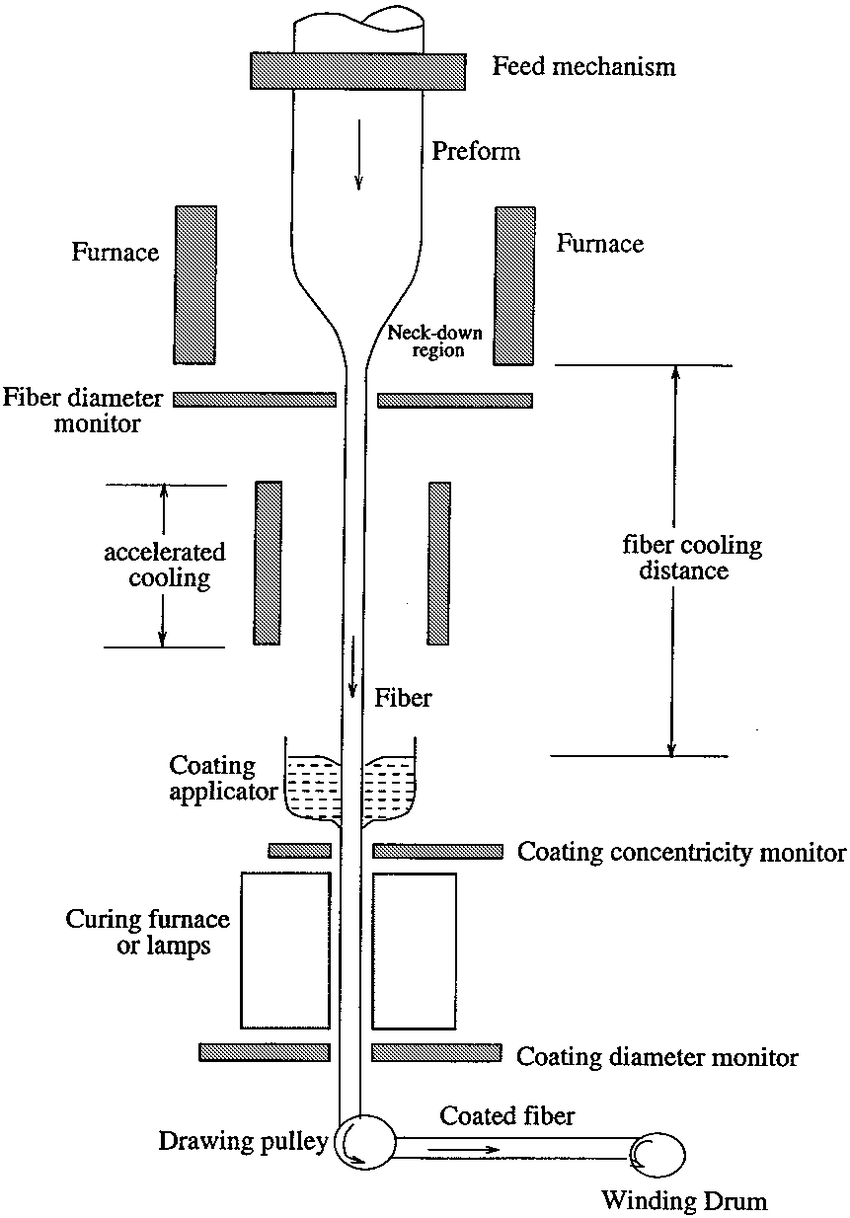
\includegraphics[width=0.75\textwidth]{figures/neckdown.png}
    \caption{A simplified illustration of a typical optical fiber drawing tower and its components \cite{neckdown}.}
    \label{fig:neckdown}
\end{figure}

A typical optical fiber drawing tower is illustrated in Figure \ref{fig:neckdown}. The fiber extrusion system in this study employs a thermal drawing technique. The process begins with a cylindrical preform rod, which is made of optical glass, being fed into a radiative furnace. The preform becomes heated and malleable, which enables it to form the neck-down profile axially and flow from a preform diameter of a few centimeters to optical fiber of micron-level diameter \cite{neckdown}. A supply of helium gas is injected into the furnace to cool down and solidify the glass fiber. The capstan assembly at the bottom pulls it with a specified tension force and velocity to produce the finished product, a spool of fiber wounded up at the end of the process. Multiple sensors also work to monitor the real-time states of the fiber drawing system, among which are the temperature of the furnace, bare fiber diameter (BFD), and velocity and tension at the capstan pulley. 

\begin{figure}[ht!]
    \centering
    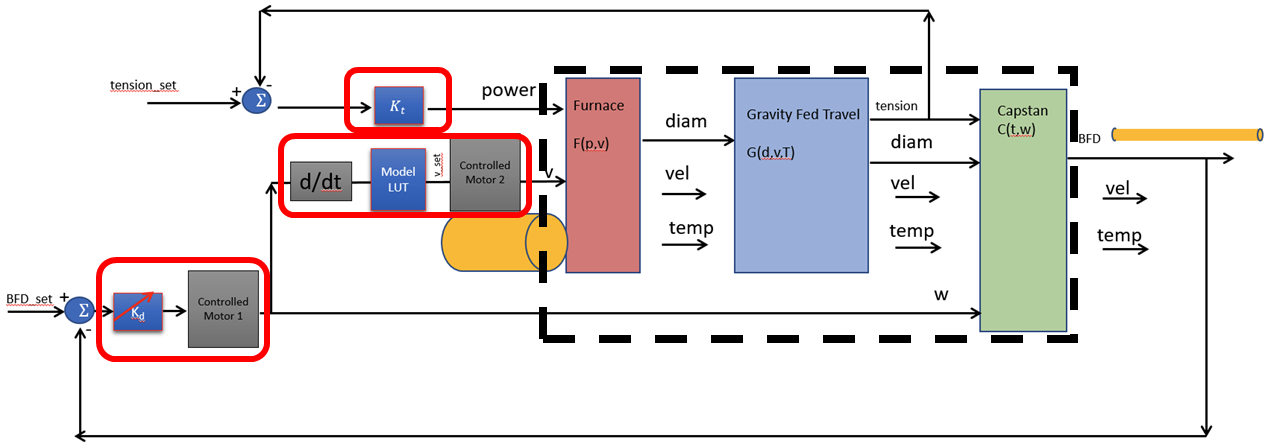
\includegraphics[width=\textwidth]{figures/stl_system_diag.png}
    \caption{Schematic diagram of the optical fiber drawing system from Sterlite Technologies Ltd. The red solid boxes indicate the three controllers, and the black dashed box indicates the aggregate fiber drawing plant to be identified.}
    \label{fig:stl_system_diag}
\end{figure}

A schematic diagram of Sterlite's fiber drawing system is shown in Figure \ref{fig:stl_system_diag}. There are three controllers modulating the signals involved in the fiber extrusion process. The tension controller, labeled as $K_t$ in Figure \ref{fig:stl_system_diag}, is a Proportional-Integral-Derivative (PID) controller that takes the error in measured tension as input and outputs the power signal to the radiative furnace. The diameter controller, labeled as $K_d$ in Figure \ref{fig:stl_system_diag}, is also a PID controller that takes the error in BFD and has capstan speed as its output. The preform velocity controller (the middle red box in Figure \ref{fig:stl_system_diag}) involves a discrete lookup table that correlates the slope of the capstan speed (i.e. acceleration) to the feed speed of the preform. Tension force during the neck-down process and the real-time BFD are measured by sensors for feedback control. 

\section{Previous Work}

There is an ample amount of literature investigating fiber manufacturing systems. The fluid dynamics and heat transfer problems involved in the fiber drawing process are well-studied; its governing equations can be derived from constitutive relations and fundamental conservation laws \cite{fiber_fluids1,fiber_fluids2,fiber_fluids3,fiber_fluids4}. The control problems of process variables (e.g. temperature of molten glass, winding speed, ambient temperature, etc) are also formulated \cite{fiber_ctrl1, fiber_ctrl2}. However, most controller design studies in the manufacturing field are developed from first principles \cite{manu_ctrl1, manu_ctrl2, manu_ctrl3}; the data-driven approach to controller design has yet to be fully explored. 

In addition, David Donghyun Kim developed a desktop fiber manufacturing system as part of his doctoral research in MIT's Device Realization Lab \cite{ddkim_phdthesis}. The implication of this system is threefold: 
\begin{enumerate}
    \item To gather measurement data that mimic the fiber extrusion process in production;
    \item To serve as a research platform for prototyping low-cost components and manufacturing techniques;
    \item To provide educational value to teach fundamentals on manufacturing, feedback controls, machine learning, and more.
\end{enumerate}

In addition, Sangwoon Kim also developed a deep reinforcement learning approach for tracking control of the fiber extrusion process, implemented with the desktop prototyping hardware \cite{sangwoon}. Although this thesis concerns about the full-scale, production-grade fiber draw tower in Sterlite, the approach for modeling and simulating the process dynamics can be applicable to the prototyping hardware, which can be used as a validation tool as well.  


\section{Thesis Overview}\label{ch:intro:thesis_ov}

This thesis details the development of models for the aggregate plant (i.e. the black box in Figure \ref{fig:stl_system_diag}) and each of the controllers (i.e. the red boxes in Figure \ref{fig:stl_system_diag}) in the optical fiber drawing system. 

The process dynamics of the aggregate plant is modeled with a black-box, neural network approach. The fiber extrusion process involving the radiative furnace, gravity fed travel, and the capstan assembly is treated as a black box, since it can be collectively described by a set of heat transfer and fluid dynamics equations. The input-output relationship of the black-box system is obtained by training neural networks of various configurations. Chapter \ref{ch:ml} presents the theoretical background of Long Short-Term Memory (LSTM) neural networks and machine learning in general. Chapter \ref{ch:exp} describes the experiments conducted to obtain said black-box correlation, and our metric to verify the model's generalizability and robustness. 

The modeling and simulation for the three controllers, mentioned in Section \ref{ch:intro:fiber}, are developed using statistical time-series system identification methods, namely Output-Error (OE) and AutoRegressive Moving Average model with eXogenous inputs (ARMAX). Chapter \ref{ch:sysid} details the theoretical background for these methods, the procedure by which a model's orders and parameters are determined, and the evaluation criteria that selects a model for simulation. The results of the identification process on the bare fiber diameter controller are also presented as a comprehensive case study.

The closed-loop simulation connecting all components of this work is found in Chapter \ref{ch:res}, along with a discussion on explainability of neural networks and time-series models through the lens of classical control. The implications of this work are also discussed, namely the usability of the closed-loop simulation as a design tool for controller improvements. This thesis ends with a discussion admitting the limitations of this work and a conclusion enumerating the potential areas that warrant further research in this ongoing project. 

% \begin{eqnarray*}
% a_i & = & a_j + a_k \\
% a_i & = & 2a_j + a_k \\
% a_i & = & 4a_j + a_k \\
% a_i & = & 8a_j + a_k \\
% a_i & = & a_j - a_k \\
% a_i & = & a_j \ll m \mbox{shift}
% \end{eqnarray*}
% instead of the multiplication.  For example, you could use:
% \begin{eqnarray*}
% r & = & 4s + s\\
% r & = & r + r
% \end{eqnarray*}
% Or by xx:
% \begin{eqnarray*}
% t & = & 2s + s \\
% r & = & 2t + s \\
% r & = & 8r + t
% \end{eqnarray*}

\chapter{Machine Learning as a Modeling Tool} \label{ch:ml}

Machine learning is a branch of artificial intelligence which focuses on using statistical methods to infer relationships, make classifications and predict outcomes. Through increased experience and use of observational data, a learned model can improve its prediction accuracy. There are three types of commonly used methodologies for learning models: 

\begin{enumerate}
    \item \textbf{Supervised learning.} This methodology learns a model based on labeled data. The learning algorithm trains and validates the model against the known ground truth. 
    \item \textbf{Unsupervised learning.} This approach identifies patterns, structures, and features within the data without labels. The algorithm can organize data via clustering, association, autoencoders, and other methods \cite{nvidia}.
    \item \textbf{Reinforcement learning.} An environment and possible discrete states are defined for an agent to transition from one state to another. After the agent takes an action, it gets some amount of reward upon some metric of success, and no reward (or even penalty) upon failure. In doing so, the agent learns the best policy to interact with the environment. 
\end{enumerate}

In this work, a supervised approach is utilized to identify the correlation between inputs and outputs of a black-boxed fiber drawing plant model. After a brief overview of the nomenclature and theory behind neural networks in Section \ref{ch:ml:nn}, Section \ref{ch:ml:rnn} provides the theoretical foundation of this approach, namely a subset of recurrent neural networks called Long Short-Term Memory (LSTM) networks and its variants. 

\section{Preliminaries} \label{ch:ml:nn}

\subsection{Nomenclature and Definitions} \label{ch:ml:nn:def}

The computational paradigm of artificial neural networks (ANNs) draws inspiration from biological neural systems, such as the human brain, to model information flow. A neural network\footnote{Artificial neural networks and neural networks are treated as interchangeable terms.} consists of interconnected elements referred to as \emph{neurons}. A neuron maps a vector of $m$ inputs $\mathbf{x}=\left[x_1, x_2, ..., x_m\right]^T \in \mathbb{R}^{m}$ to a scalar output value $a\in \mathbb{R}$. It is parametrized by a vector of weights $\mathbf{w}=\left[w_1, w_2, ..., w_m\right]^T \in \mathbb{R}^{m}$, in which each element is associated with the input $\mathbf{x}$ at the corresponding index, and the \emph{bias}\footnote{In literature it may be referred to as \emph{offset}, \emph{threshold}, or others.} $w_0$. A neuron is also associated with an \emph{activation function} $f(z): \mathbb{R} \rightarrow \mathbb{R}$, such that\footnote{Some literature writes simply $f\left(\mathbf{w}^T\mathbf{x}\right)$ where  $\mathbf{w}$ and $\mathbf{x}$ has $w_0$ and $x_0$ prefixed into the vector defined above, and $x_0$ is permanently defined as $1$, which yields meaningful calculations in the case of a nonzero bias term \cite{mackay_nn}.}

\begin{equation}
    \label{eqn:activ_fcn}
    a = f(z) = f\left( \sum_{i=1}^n x_i w_i + w_0\right) = f\left(\mathbf{w}^T\mathbf{x} + w_0\right) 
\end{equation}

Some of the most commonly used activation functions are listed in Table \ref{tab:activ_fcns}. The choice of activation function depends specifically on the use case. For instance, LSTM networks, which will be introduced in Section \ref{ch:ml:rnn:lstm}, primarily use sigmoid and hyperbolic tangent activation functions within its structure. Figure \ref{fig:neuron} depicts the basic structure of a single neuron and all operations discussed above. 

\begin{figure}
    \centering
    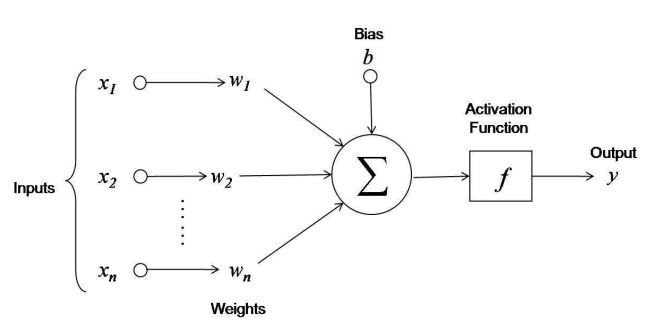
\includegraphics[width=0.9\textwidth]{figures/neuron.jpeg}
    \caption{Illustration of a single neuron and its operations within \cite{neuron}.}
    \label{fig:neuron}
\end{figure}

\begin{figure}
    \centering
    \resizebox{\textwidth}{!}{
    \begin{tikzpicture}
    
    % Input Layer
    \foreach \i in {1,...,2}
    {
    	\node[circle, 
    		minimum size = 6mm,
    		fill=cyan!30] (Input-\i) at (0,-\i) {};
    }
    
    % Hidden Layer
    \foreach \i in {1,...,5}
    {
    	\node[circle, 
    		minimum size = 6mm,
    		fill=gray!50,
    		yshift=3*5 mm
    	] (Hidden1-\i) at (2.5,-\i) {};
    }
    
    \foreach \i in {1,...,5}
    {
    	\node[circle, 
    		minimum size = 6mm,
    		fill=gray!50,
    		yshift=3*5 mm
    	] (Hidden2-\i) at (5,-\i) {};
    }
    
    % Output Layer
    \foreach \i in {1,...,2}
    {
    	\node[circle, 
    		minimum size = 6mm,
    		fill=green!50,
    		yshift=0*5 mm
    	] (Output-\i) at (7.5,-\i) {};
    }
    
    % Connect neurons In-Hidden
    \foreach \i in {1,...,2}
    {
    	\foreach \j in {1,...,5}
    	{
    		\draw[->, shorten >=1pt] (Input-\i) -- (Hidden1-\j);	
    	}
    }
    
    \foreach \m [count=\y] in {missing}
      \node [every neuron/.try, neuron \m/.try ] (hidden-\m) at (3.725,-1.625) {};
    
    % Connect neurons Hidden-Out
    \foreach \i in {1,...,5}
    {
    	\foreach \j in {1,...,2}
    	{
    		\draw[->, shorten >=1pt] (Hidden2-\i) -- (Output-\j);
    	}
    }
    
    % Inputs
    \foreach \i in {1,...,2}
    {            
    	\draw[<-, shorten >=1pt] (Input-\i) -- ++(-1,0)
    		node[left]{$x_{\i}$};
    }
    
    % Outputs
    \foreach \i in {1,...,2}
    {            
    	\draw[->, shorten >=1pt] (Output-\i) -- ++(1,0)
    		node[right]{$y_{\i}$};
    }
    \end{tikzpicture}
    }
    \caption{Illustration of a feedforward neural network. The input, hidden, and output layers are shown in cyan, gray, and green, respectively.}
    \label{fig:nn}
\end{figure}

\begin{table}
    \centering
    \begin{tabular}{c|c|c}
        \textbf{Activation Function} & \textbf{Graph} & \textbf{Usage} \\ \hline \hline
        \makecell{Step function\\ 
        step$(z) =$
            \[\begin{cases} 
                  0 & z < 0 \\
                  1 & z\geq 0 
               \end{cases}
            \]
        }
        & \makecell{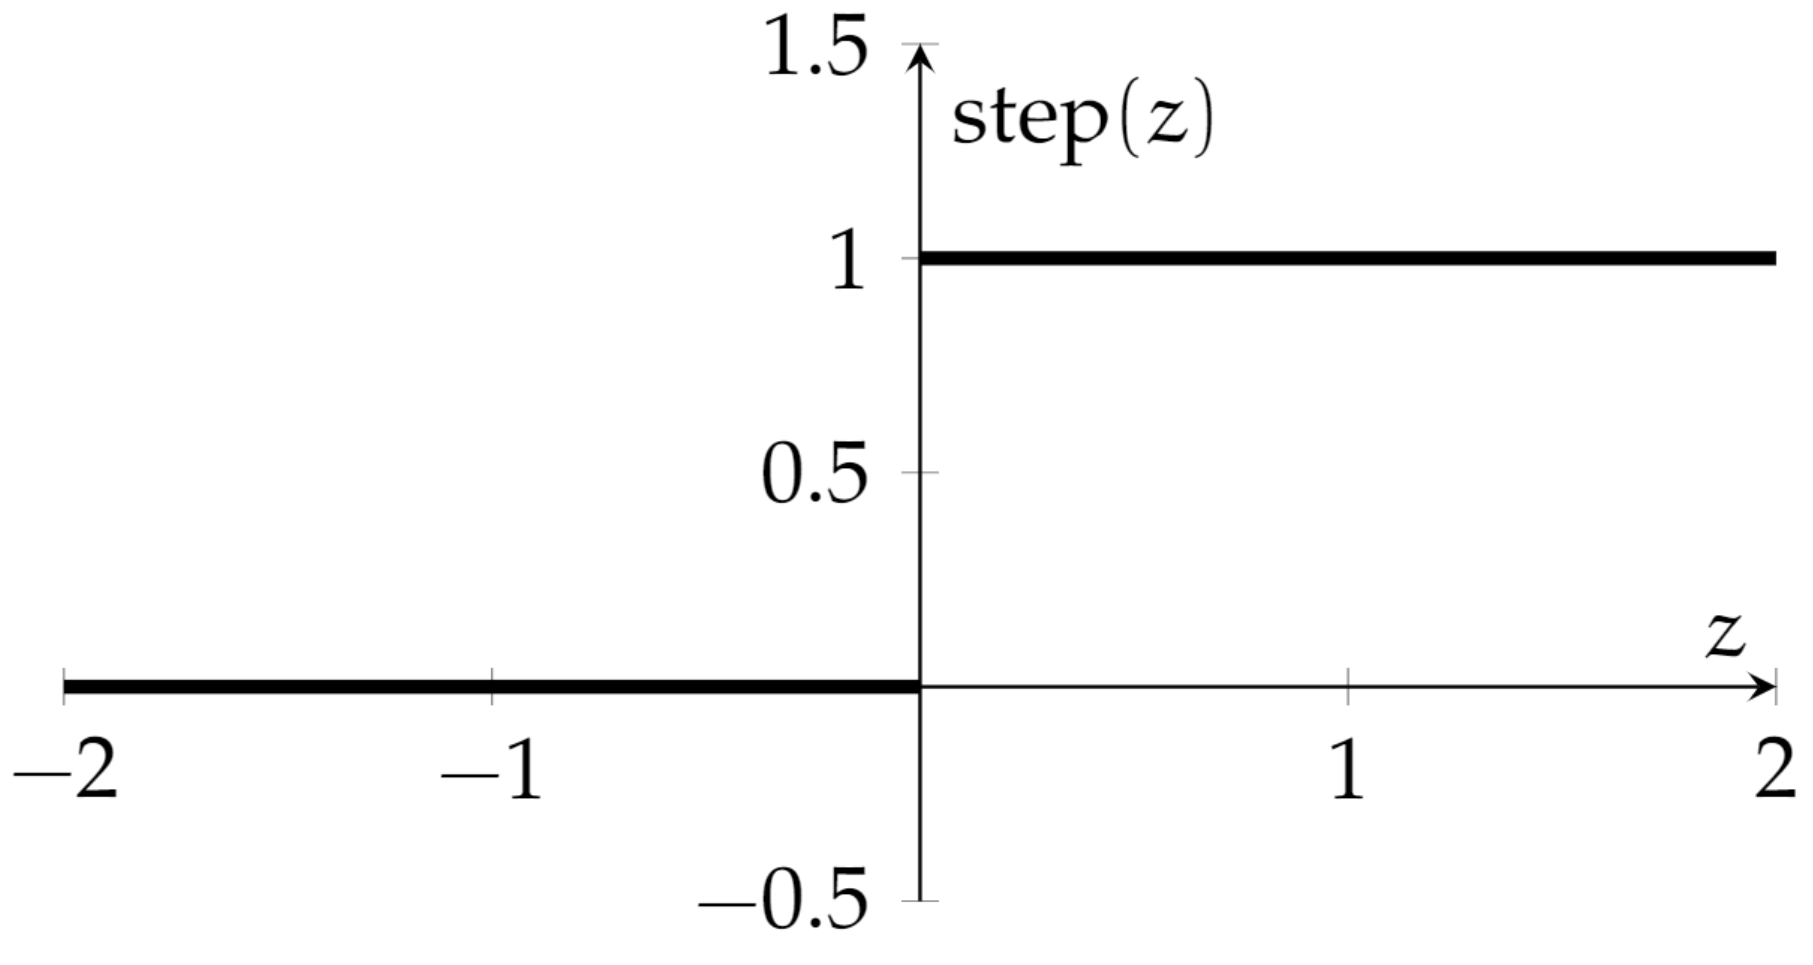
\includegraphics[width=4cm]{figures/step.png}} & Binary (0-1) loss \\ \hline
        
        \makecell{Linear Function\\ \\
        $f(z) = z$
        }
        & \makecell{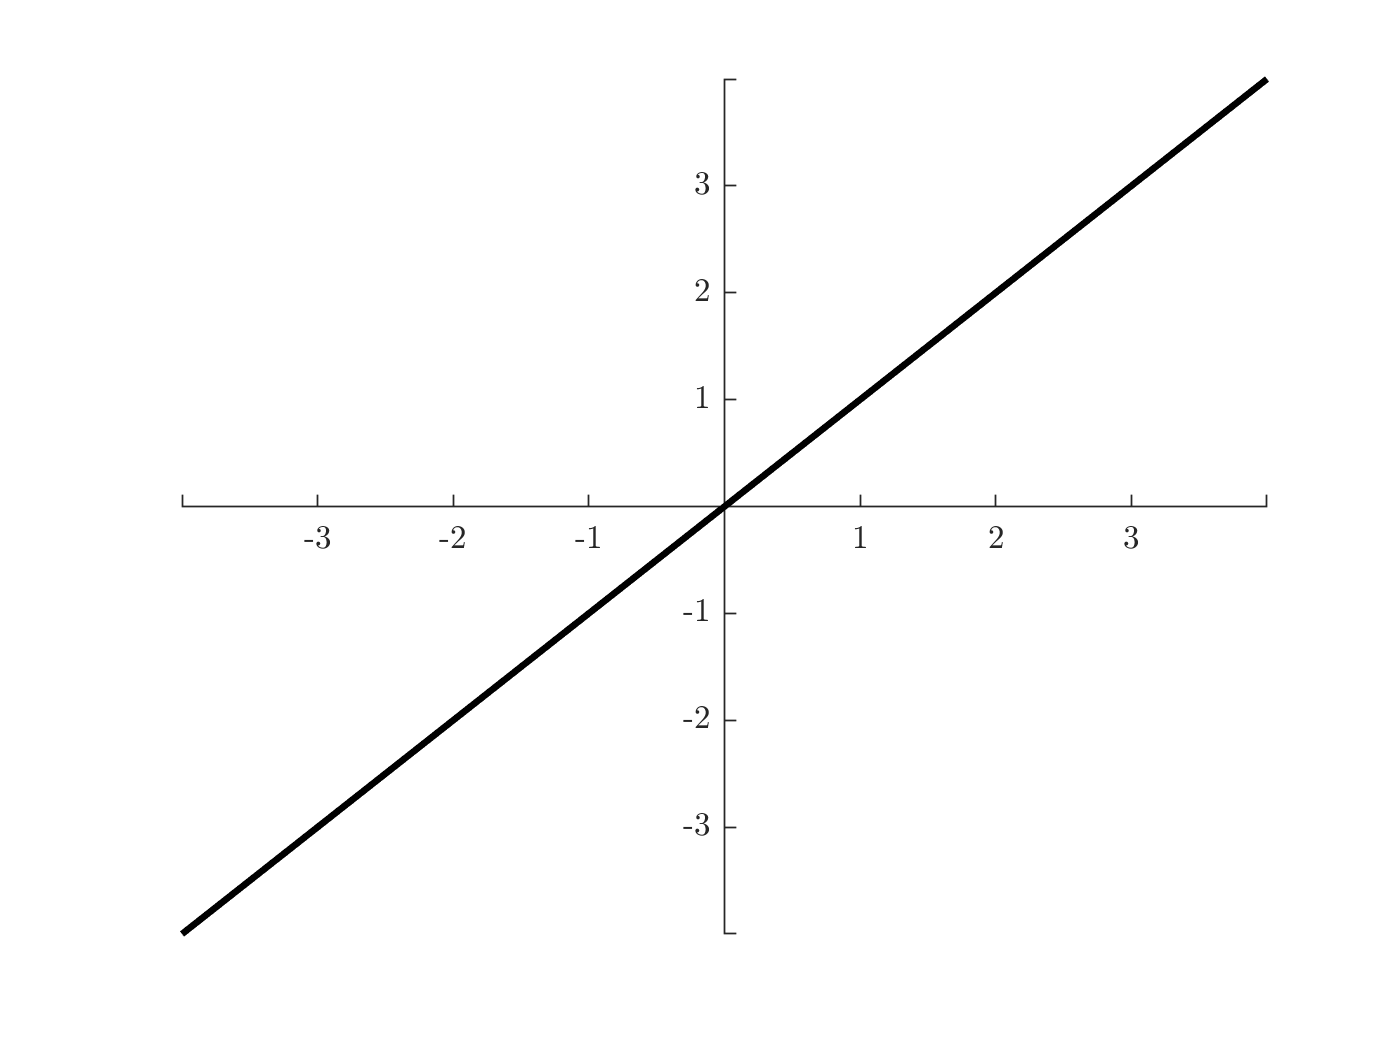
\includegraphics[width=3cm]{figures/linear.png}} & Passthrough \\ \hline
        
        \makecell{Sigmoid/Logistic function\\ \\
        $\sigma(z) = \dfrac{1}{1+e^{-z}}$
        }
        & \makecell{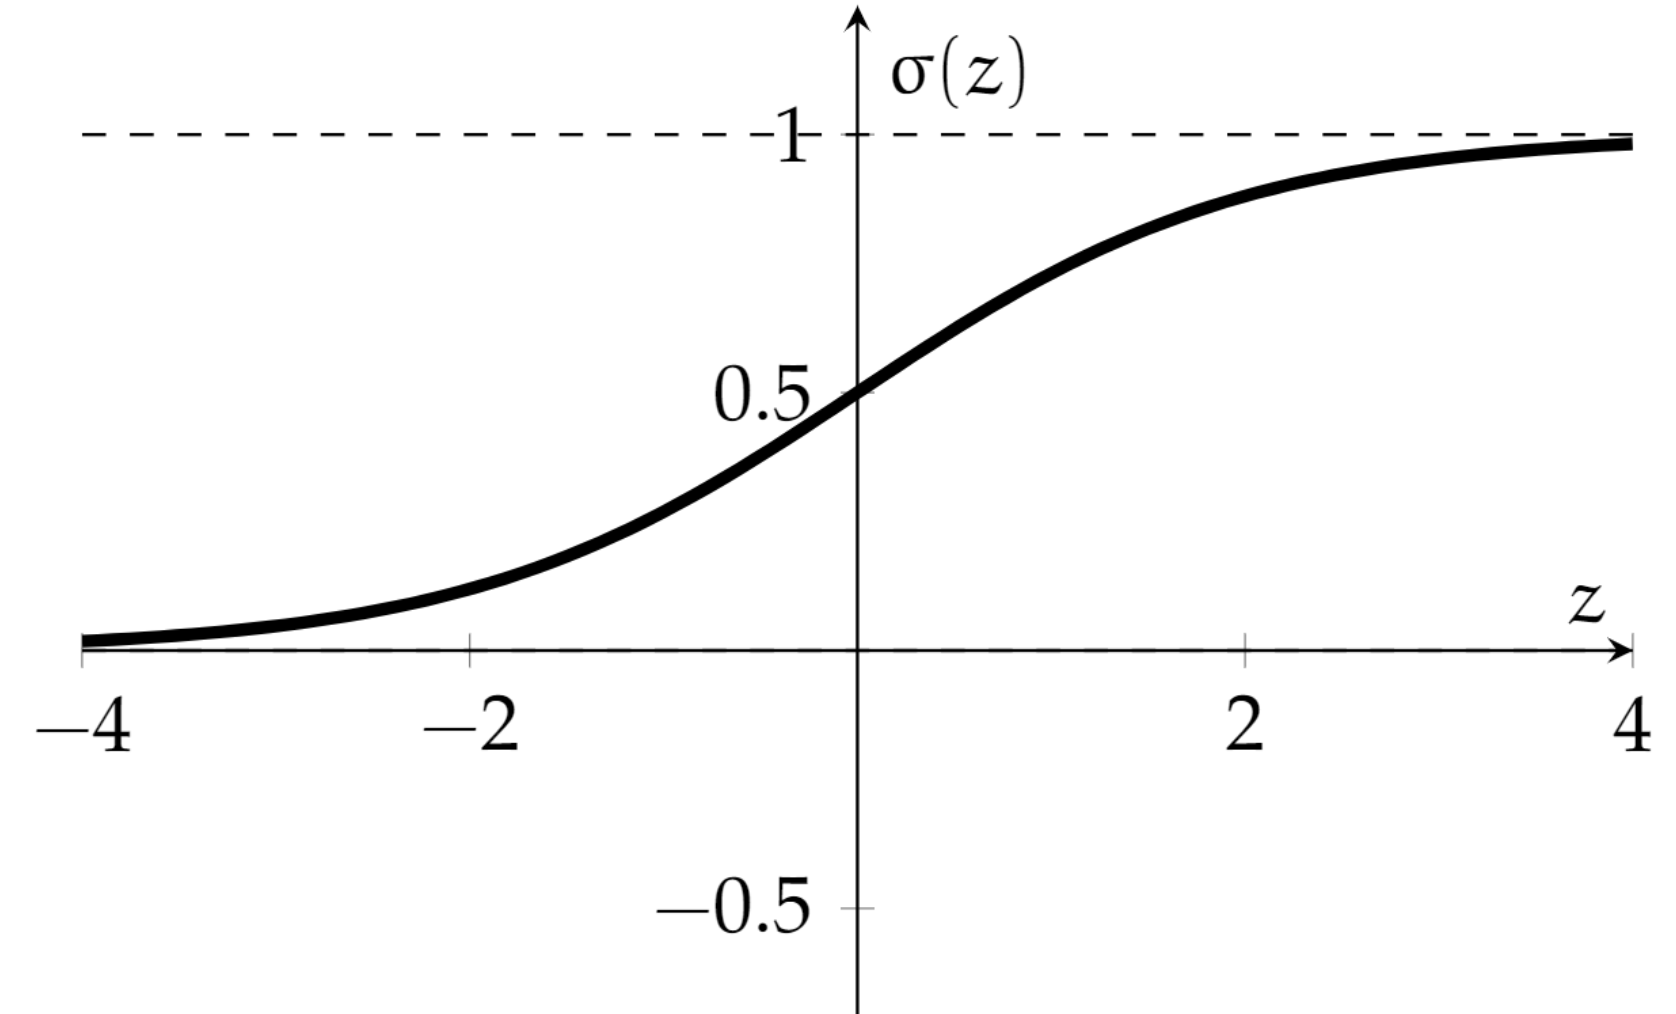
\includegraphics[width=4cm]{figures/sigmoid.png}} & Regression \\ \hline
        
        \makecell{Hyperbolic Tangent (tanh)\\ \\
        $\tanh(z) = \dfrac{e^z-e^{-z}}{e^z+e^{-z}}$
        }
        & \makecell{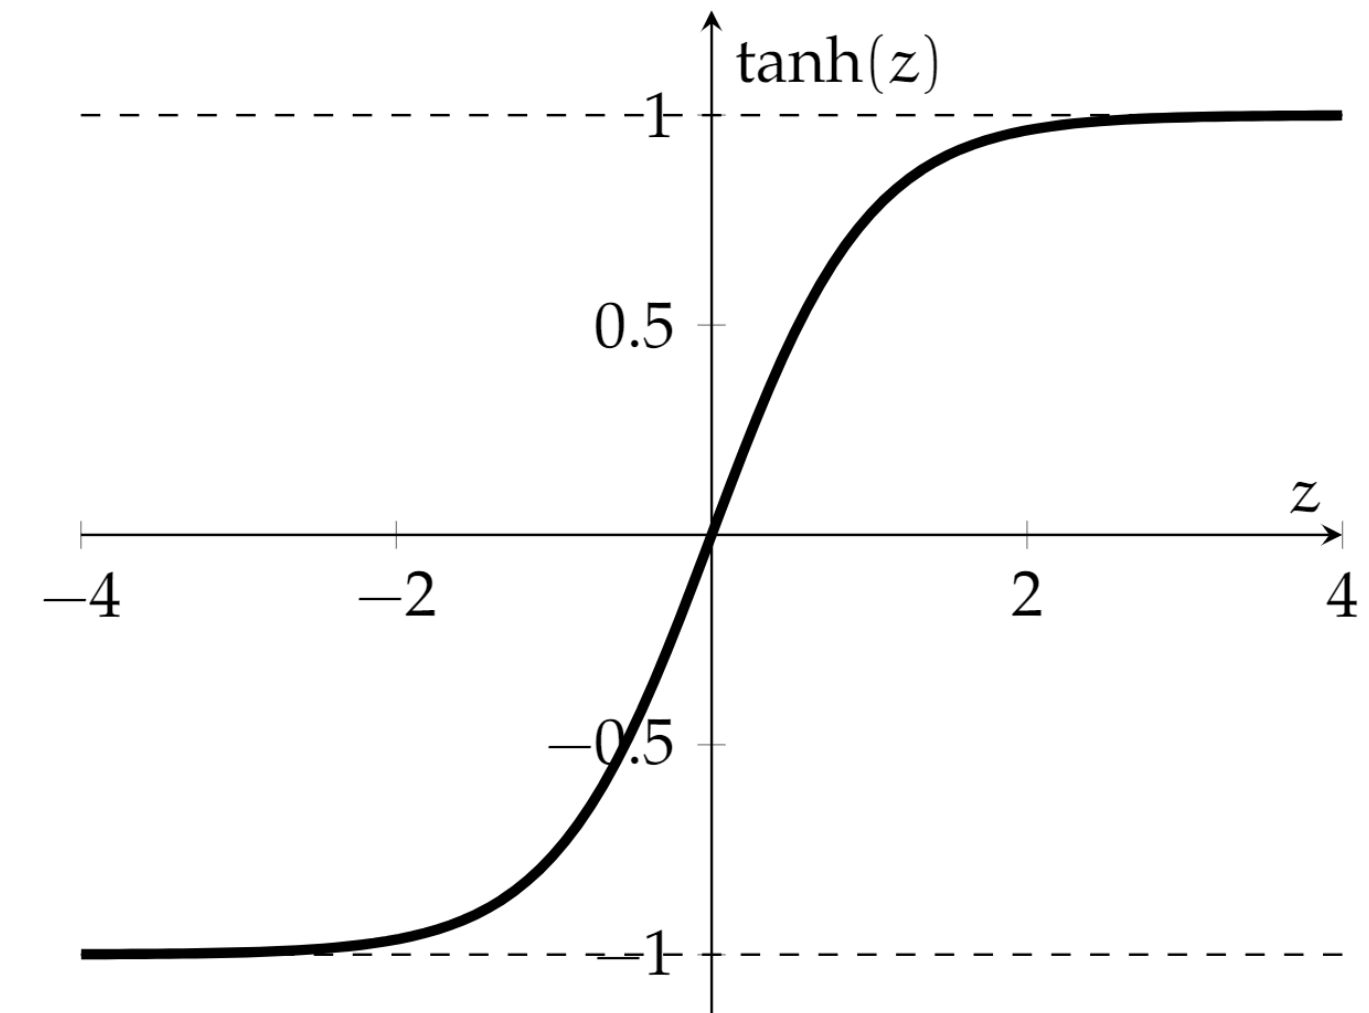
\includegraphics[width=4cm]{figures/tanh.png}} & Normalizing data \\ \hline
        
        \makecell{\\Softmax function\\ \\
        $\text{softmax}(\mathbf{z}) = \dfrac{\exp(\mathbf{z})}{\sum_{j} \exp(z_j)}$\\ \\
        }
        & \makecell{N/A} & \makecell{Multi-class \\ classification} \\ \hline
        
        \makecell{\\Rectified Linear Unit (ReLU)\\ \\
        ReLU$(z) = $
            \[\begin{cases} 
                  0 & z < 0 \\
                  z & z\geq 0 
               \end{cases}
            \] = \max(0,z) \\ \\
        }
        & \makecell{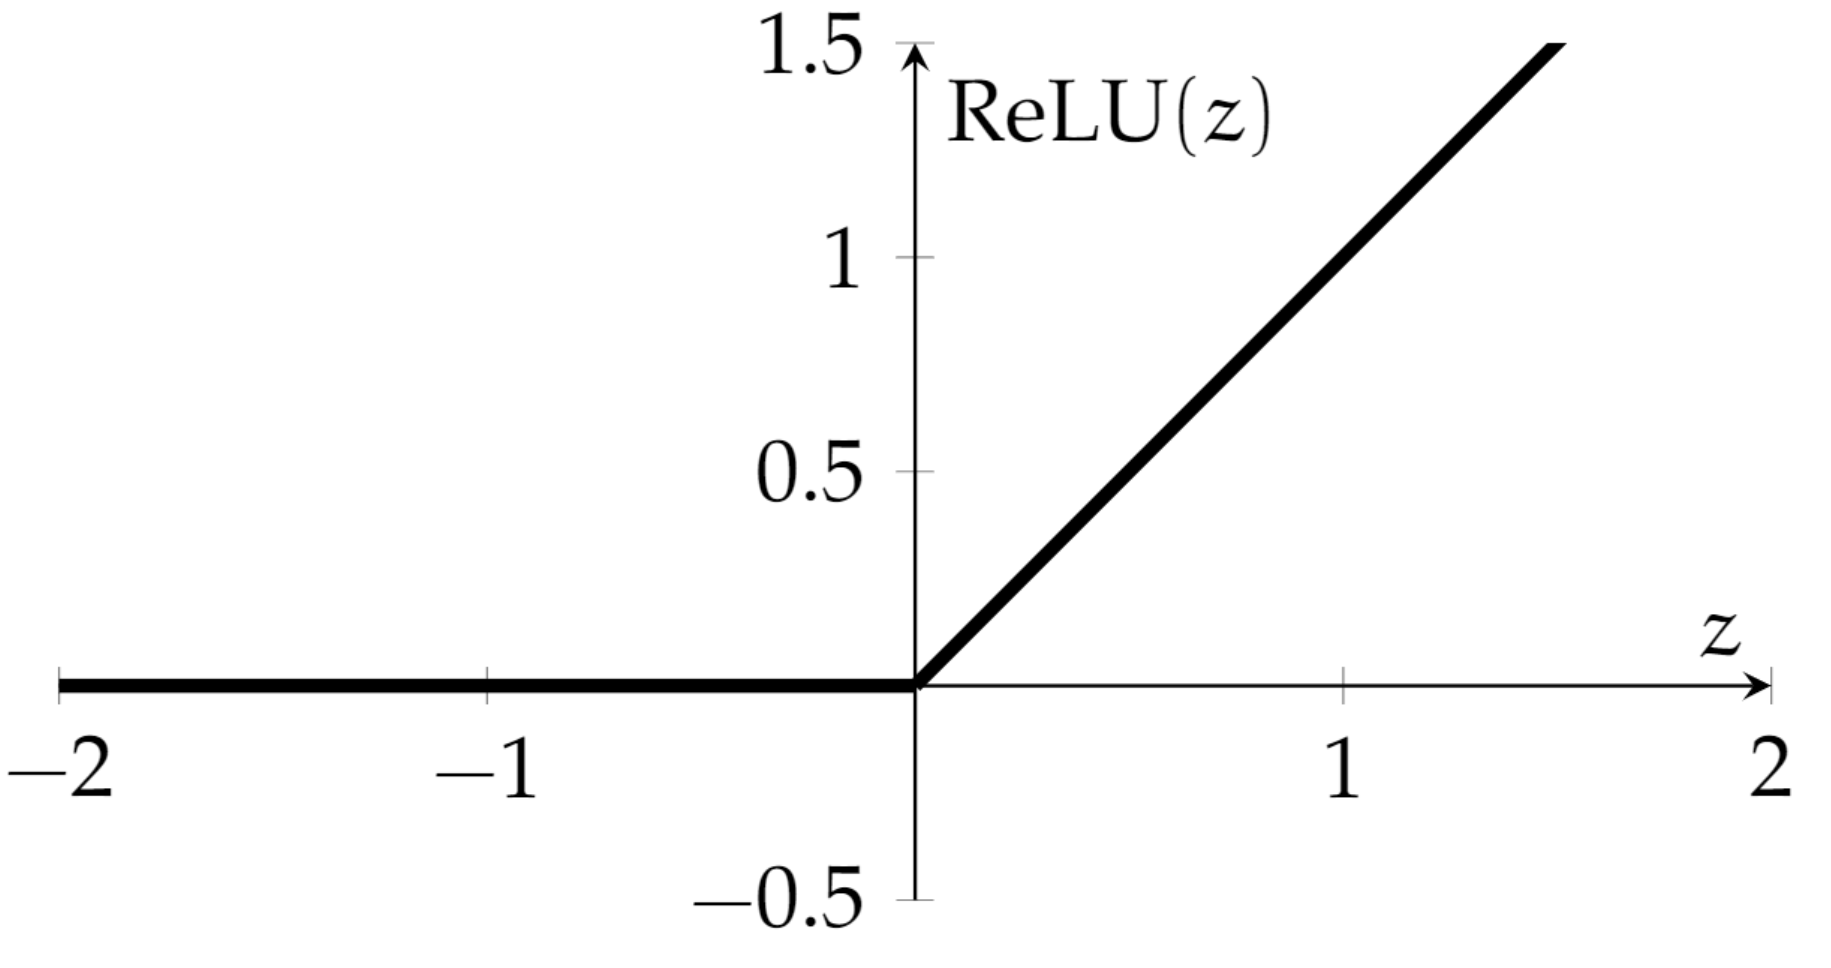
\includegraphics[width=4cm]{figures/ReLU.png}} & CNNs \\ \hline
        
        \makecell{Leaky ReLU\\ \\
        LReLU$(z) = $
            \[\begin{cases} 
                  \alpha z & z < 0 \\
                  z & z\geq 0 
               \end{cases}
            \], $\alpha > 0$
        }
        & \makecell{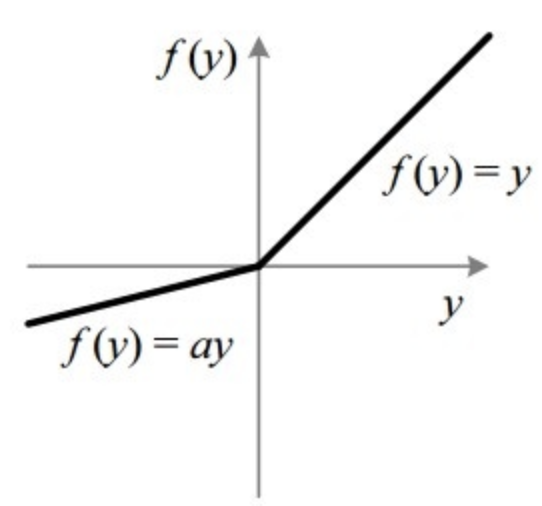
\includegraphics[width=4cm]{figures/leaky_relu.png}} & CNNs \\ \hline
        
    \end{tabular}
    \caption{A table of common activation functions, their equations, graphs, and usages\cite{6036}.}
    \label{tab:activ_fcns}
\end{table}

Figure \ref{fig:nn} illustrates the basic anatomy of a \emph{feed-forward neural network}, rightfully named so since its information only flows in the forward direction. Each vertical stack of neurons is called a \emph{layer}. The first layer is called the \emph{input layer}; the layer at which the outputs are generated is called the \emph{output layer}. All intermediate layers in between are called \emph{hidden layers}, and they often represent intermediate or internal representations of the information. For a layer with $n$ units (therefore $n$ outputs) and $m$ inputs, we can denote the weight matrix $\mathbf{W}$ of this particular layer as an $m\times n$ matrix\footnote{Aligning with conventional standards, uppercase bold letters indicate matrices and lowercase bold letters indicate vectors.}, and the output of this layer is expressed as

\begin{equation}
    \label{eqn:layer}
    \mathbf{a} = f(\mathbf{z}) = f\left( \sum_{i=1}^n \mathbf{W}^T\mathbf{x} + \mathbf{w}_0\right) 
\end{equation}
where the bias vector $\mathbf{w}_0 \in \mathbb{R}^n$ and layer output $\mathbf{a} \in \mathbb{R}^n$. 

Recently, a machine learning technique known as \emph{deep learning} has been gaining popularity. Deep neural networks are ones with a large amount of hidden layers, potentially as many as 150. Deep learning has been proven to outperform traditional learning algorithms when presented with a large amount of data \cite{andrew_ng}. The increased parameter space in deep neural networks naturally lends itself to more complex problems such as speech recognition, image classification, and natural language processing. 


\subsection{Supervised Training} \label{ch:ml:nn:train}

Neural networks are often utilized in supervised learning to solve a classification or regression problem. Through the training process, the weights within the neural network are learned to minimize the \emph{loss function}\footnote{Also known as the \emph{objective function} or \emph{cost function} in literature.} $J$, which measures how accurate each of the network outputs are to the corresponding label. Loss functions may take many forms; a selected list of the most common cost functions are enumerated in Table \ref{tab:loss_fcns}. 

% MIGHT REMOVE BOTH TABLES 
\begin{table}[]
    \centering
    \resizebox{\textwidth}{!}{
    \begin{tabular}{c|c|c}
         Name & Equation & Usage  \\ \hline
         
         Binary loss & $L(y,\hat{y}) = $
            \[\begin{cases} 
                  0 & y=\hat{y} \\
                  1 & otherwise 
               \end{cases}
            \]
            & Finite domains \\ 
        
        Linear/L1 loss & $L(y,\hat{y}) = |y-\hat{y}|$ & Regression with outliers \\ 
        Squared/L2 loss & $L(y,\hat{y}) = (y-\hat{y})^2$ & Regression \\ 
        Cross-entropy loss & $L(y,\hat{y}) = -\left[y_i\log \hat{y}_i +(1-y_i)\log (1-\hat{y}_i)\right]$ & Classification
        
    \end{tabular}
    }
    \caption{Common loss functions.}
    \label{tab:loss_fcns}
\end{table}

In other words, training of neural networks is an optimization process in which weights are chosen to minimize the cost function. Most commonly, neural networks are trained using variants of \emph{gradient descent} approaches. The derivative of the cost function with respect to the weights $\mathbf{w}$ (also known as the \emph{network gradient}) is calculated by repeatedly applying the chain rule, in a process known as \emph{backpropagation} \cite{rumelhart_backprop}.

% maybe draw a NN, write out all derivatives, and explain back prop??

Once the network gradient is obtained, the weights are adjusted in the direction opposite to the network gradient, the sensitivity of which is parametrized by the \emph{learning rate} $\eta$. Mathematically, a parameter $\theta$ is iterated as follows, 

\begin{equation}
    \label{eqn:lr}
    \theta \leftarrow \theta - \eta \cdot \nabla_\theta J(\theta) 
\end{equation}

\begin{figure}[t!]
    \centering
    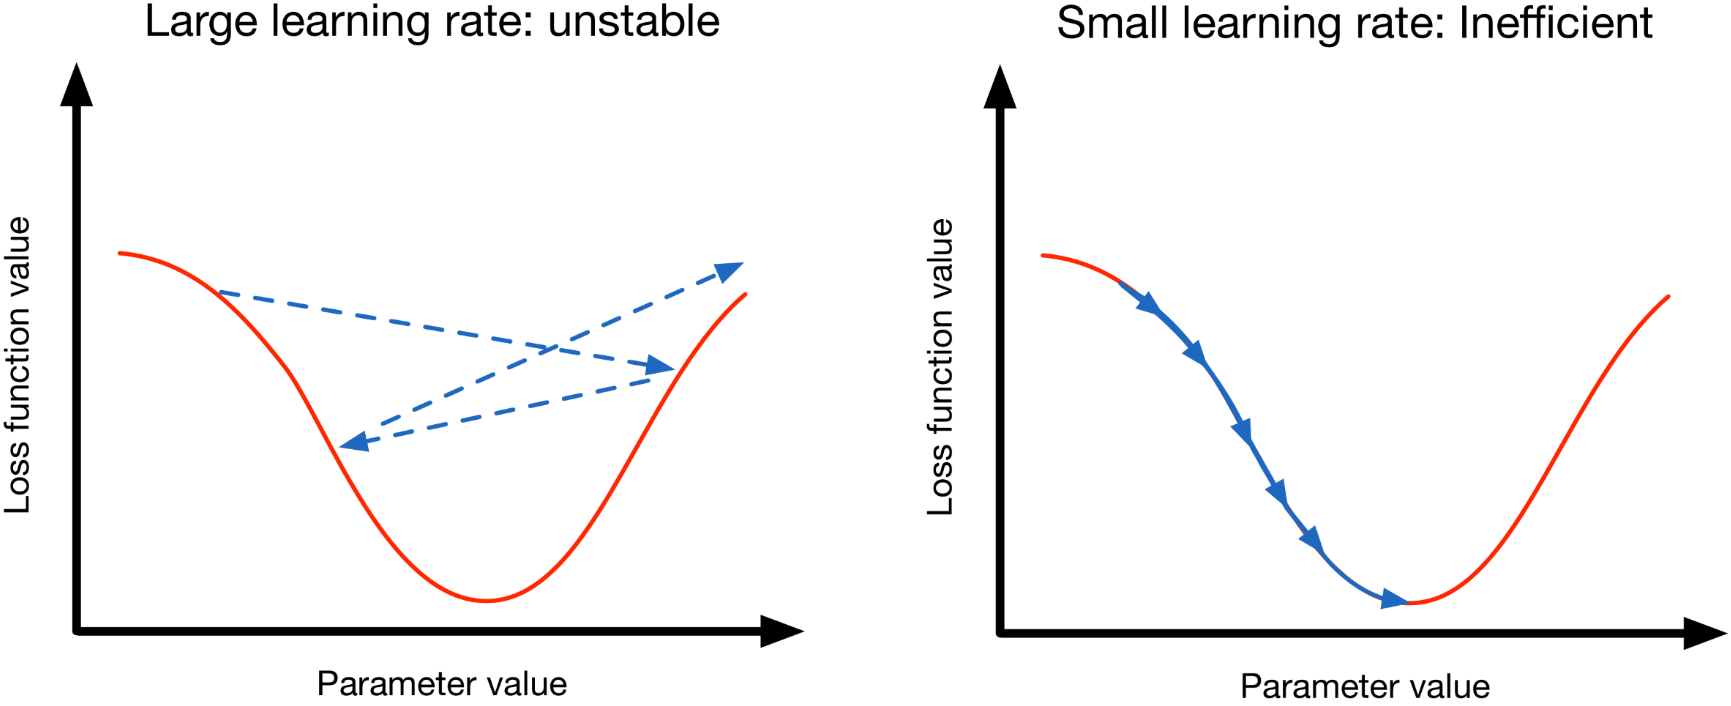
\includegraphics[width=\textwidth]{figures/lr.png}
    \caption{Effects of learning rate on loss minimization \cite{dl_patterson}.}
    \label{fig:lr}
\end{figure}

As shown in Figure \ref{fig:lr}, a learning rate too low requires many iterations and impedes the speed of learning, whereas a learning rate too high may overshoot and lead to divergent behaviors that never reach the desired minimum of the optimization landscape. Selecting an appropriate learning rate, which can converge without sacrificing the speed of learning, is more of an experimental exercise than an analytical one. Especially for deep neural networks, choosing a scheduled, adaptive learning rate can greatly accelerate the training process. There are commonly used decaying learning rate schedules such as exponential, linear, or piecewise\cite{dl_patterson}. In addition, algorithms such as Adagrad \cite{duchi_adagrad}, Adam \cite{kingma_adam}, RMSprop \cite{hinton_rmsprop}, and Nesterov Accelerated Gradient \cite{nesterov_nag}, have been widely used in many applications. 

For deep neural networks, the training process involves dividing the dataset into \emph{batches} and iterating over all the training dataset for multiple \emph{epochs}. In each iteration of an epoch, some \emph{batch size} of data are presented to the network, and the network gradient of all weights are computed based on the loss function calculated with said batches of data. The effects of these hyperparameters, such as learning rate, batch size, and number of epochs, are studied extensively with different datasets. \cite{batch_size_dynamics, batch_size} The consensus in literature suggests that large batch sizes are detrimental to the network's ability to generalize, whereas smaller batch sizes and lower learning rates are beneficial only for fine-tuning purposes, although reaching global optima is not guaranteed due to the non-convexity of the landscape. In general, these effects in the training process depends heavily on the model, the specific usage, and the datasets themselves. 

Furthermore, there are other components to training the neural network, among which are parameter regularization techniques, such as dropout and batch normalization \cite{batch_norm}. Many textbooks are written to provide guidelines to effectively process data and train neural networks. \cite{dl_patterson} and \cite{ml_book_chollet}, for example, give a comprehensive treatment on these topics. 

\section{Recurrent Neural Networks}\label{ch:ml:rnn}

\subsection{Theory of RNNs} \label{ch:ml:rnn:theory}

In contrast to feedforward neural networks discussed above, recurrent neural networks \cite{rumelhart_backprop} have internal feedback loops in their structures, as shown in Figure \ref{fig:rnn}. The feedback of information is especially important for maintain internal state(s) when processing sequential data. For this reason, RNNs have received increasing popularity across a variety of disciplines including natural language processing \cite{rnn_nlp}, speech recognition \cite{rnn_speech_recog}, machine translation \cite{rnn_machine_trans}, and many more. 

\begin{figure}[t!]
    \centering
    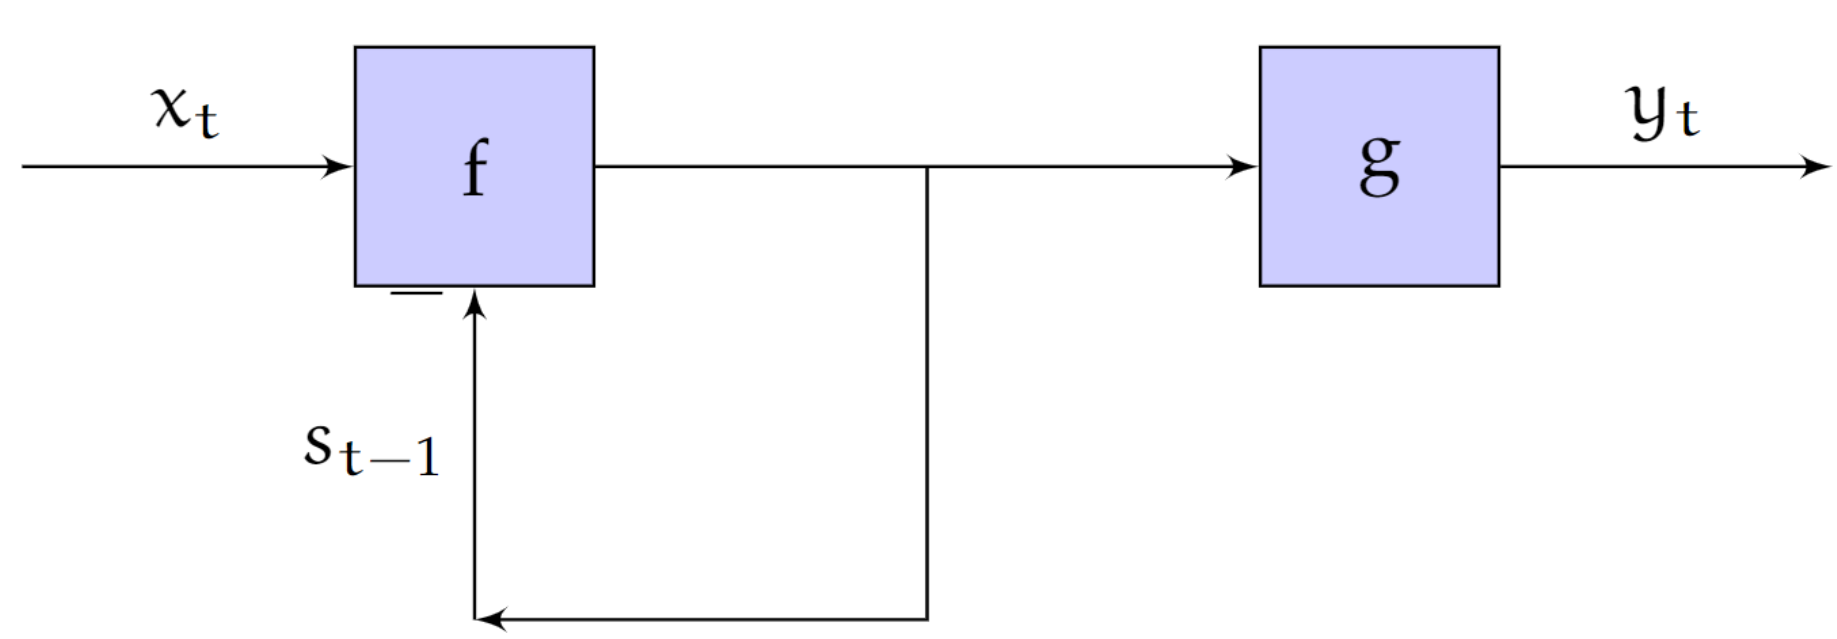
\includegraphics[width=0.7\textwidth]{figures/rnn.png}
    \caption{Structure of a simple RNN unit, modeled as a state machine.}
    \label{fig:rnn}
\end{figure}

The information flow in RNNs can be modeled as a state machine with state equations shown in Eq. \ref{eqn:rnn}. 
\begin{equation}
    \label{eqn:rnn}
    \begin{split}
        & s_t = f(s_{t-1}, u_t) \\
        & y_t = g(s_t)
    \end{split}
\end{equation}

where $s_t$ represents the state, $u_t$ the input, and $y_t$ the output at time $t$. The state activation function $f(\cdot )$ resides in the hidden layer; it represents the internal dynamics of a recurrent cell and relates the previous state and input to current state. The output activation function $g(\cdot )$ relates the current state to the output. 

The weights within RNNs are trained through an algorithm known as \emph{backpropagation through time} (BPTT), which unfolds a RNN in time and applies backpropagation (discussed in Section \ref{ch:ml:nn:train}) to find the gradient of the network cost with respect to network parameters. 

% MATH FROM https://d2l.ai/chapter_recurrent-neural-networks/bptt.html, PSEUDOCODE FROM BPTT WIKIPEDIA
% keep it brief and concise

Training RNNs, especially deep RNNs, remains a difficult task in the research community. The backpropagation (discussed in Section \ref{ch:ml:nn:train}) and, by extension, the BPTT algorithm (discussed above) suffer from the exponential growth or decay of the propagated network gradient, phenomena referred to as \emph{exploding gradient} and \emph{vanishing gradient}, respectively \cite{gradient}. 
% math behind vanishing / exploding gradient
% In other words, the error gradients are multiplied repeatedly by copies of the same weight matrix... %CHECK ON THIS
For this reason, the exploding and vanishing gradient problem impedes learning of deep neural networks, as weights closer to the beginning of the network cannot be properly updated after several iterations. There are several heuristics in literature developed to mitigate the exploding gradient problem, such as gradient clipping and weight regularization \cite{gradient}. They do, however, introduce additional hyperparameters to be tuned. Overcoming the vanishing gradient problem was proven to be even more difficult \cite{vanish_grad_difficult}. In the following subsection, I will introduce a subset of RNNs, known as Long Short-Term Memory (LSTM) networks, that partially addresses the exploding and vanishing gradient problem and is found to be better suited for time-series system identification.

\subsection{Long Short-Term Memory Networks} \label{ch:ml:rnn:lstm}

Introduced in 1997 by Hochreiter \& Schmidhuber \cite{lstm_hochreiter}, LSTM networks grew in popularity as a robust and trainable RNN model for sequential data. An illustration of a typical LSTM cell is shown in Figure \ref{fig:lstm}. In its architecture, LSTM networks consist of cells with gating mechanisms, with which the network can have "memory" and retain information over multiple timesteps. The information flow through these gates and their associated update rules are described below; in each LSTM cell, there is a

\begin{itemize}
    \item \emph{Forget gate}, which is typically a sigmoid function (refer to Table \ref{tab:activ_fcns}), that decides whether information should be forgotten (if sigmoid output is near 0) or retained (if sigmoid output is near 1). It is applied to the previous hidden state $h_{t-1}$ and produces the \emph{forget vector} $f_t$.
    \begin{equation}
        f_t = \sigma \left(W_f\cdot \left[h_{t-1},x_t\right]+b_f\right)
    \end{equation}
    \item \emph{Input gate}, which decides what new information should be stored in the cell state $C_t$. It is a combination of a sigmoid function that decides which values to update, and a tanh function that creates a vector of new candidate values.
    \begin{equation}
        \begin{split}
            i_t & = \sigma \left(W_i\cdot \left[h_{t-1},x_t\right]+b_i\right) \\
            \Tilde{C}_t & = \tanh\left(W_C\cdot \left[h_{t-1},x_t\right]+b_C\right) \\
            C_t & = f_t\cdot C_{t-1} + i_t \cdot \Tilde{C}_t
        \end{split}
    \end{equation}
    \item \emph{Output gate}, which multiplies the sigmoid-filtered hidden state and the tanh-filtered cell state $C_t$. The output is the next hidden state $h_t$. 
    \begin{equation}
        \begin{split}
            o_t & = \sigma \left(W_o\cdot \left[h_{t-1},x_t\right]+b_o\right) \\
            h_t & = o_t \cdot \tanh(C_t)
        \end{split}
    \end{equation}
    where $W$'s and $b$'s are the weight parameter matrix and bias terms, respectively, associated with each variable.
\end{itemize}

\begin{figure}[b!]
    \centering
    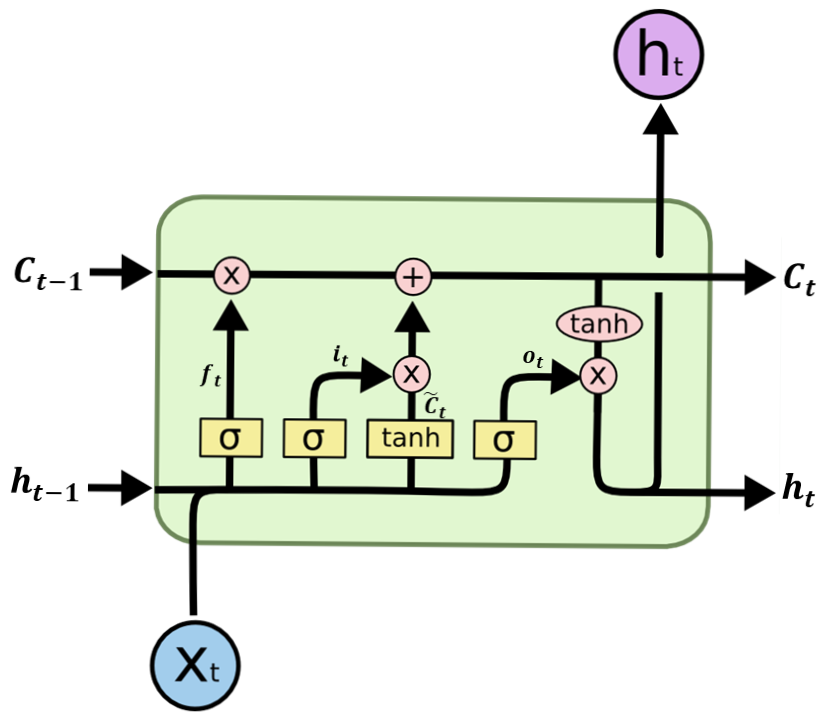
\includegraphics[width=0.6\textwidth]{figures/lstm.png}
    \caption{Illustration of a typical LSTM cell and the operations within \cite{lstm_olah}.}
    \label{fig:lstm}
\end{figure}

Besides the vanilla version of LSTM network discussed above, other variants have also been introduced. One of such variants explored in this work is the \emph{bidirectional LSTM} (biLSTM) network \cite{brnn_schuster}, which examine the data from beginning to end and from end to beginning. With each input flowing in two directions, the network preserves past and future information. Training two LSTM structures allows the learning algorithm to increase the amount of information available and provide more context to the network. This methodology of learning bidirectional dependencies within sequential data has demonstrated success in speech recognition, forecast prediction, and other signal-based machine learning problems  \cite{bilstm_speech, bilstm_speech2, bilstm_pred}. 

Gonzalez and Yu's work \cite{gonzalez} also explored a rectangular array of LSTM networks and achieved improved performance. The rectangular arrays stacked height-wise resulted in a lower root-mean-square error than the ones stacked width-wise. Parts of the experiments with network architectures are inspired by these cited literature and their performance will be evaluated in Chapter \ref{ch:exp}. 

\section{Relation to System Dynamics Modeling} \label{ch:ml:relation}

Evidently, the mathematics behind ANNs is well-developed and understood. In recent years, the rapid advancement in computational power and explosion in volume of enriching data have added incredible momentum for the machine learning community. ANNs have been used in finance \cite{ann_finance}, medicine \cite{ann_med}, and manufacturing \cite{ann_manu} alike. It has also gained popularity in the controls community for system identification purposes. An advantage of fitting the data to an LSTM model is that the nonlinear system representation can be obtained without the full knowledge of the system \cite{wagh}, which makes the black-box modeling approach plausible. An increasing amount of papers \cite{gonzalez, wang} justify this kind of usage by pointing to the \emph{Universal Approximation Theorem} (UAT), presented below.

\begin{theorem} \label{thm:uat}
\textbf{- Universal Approximation Theorem}

Let $I_m$ denote the $m$-dimensional unit hypercube $[0,1]^m$, and $C(I_m)$ denote the space of continuous functions in $I_m$. Let $\varphi(t)$ be a bounded, continuous function, $\alpha_i, b_i \in \mathbb{R}$, and the weights $w_i\in \mathbb{R}^m$. For any continuous function $f\in C(I_m)$ and $\varepsilon>0$, there exists an integer $N$ (namely, the number of neurons in a layer) such that we may define

\begin{equation}
    F(x) = \sum_{i=1}^N \alpha_i \cdot \varphi(w_i^T x + b_i)
\end{equation}

to be an approximate realization of $f$ arbitrarily close, i.e.

\begin{equation}
    |F(x)-f(x)| < \varepsilon, \texttt{    } \forall x\in I_m
\end{equation}

\end{theorem}

The original UAT \cite{cybenko_1989} guaranteed arbitrary approximation accuracy only for feedforward neural networks with one hidden layer and sigmoid-like activation functions. In 1991, Hornik et al. expanded this notion to multilayer feedforward networks with any activation functions. \cite{hornik_uat} This is a powerful result — it demonstrates that neural networks are universal approximators that can "learn" any continuous function to arbitrarily close accuracy. 

The UAT, therefore, validates the capability of neural networks to model system dynamics, especially nonlinear dynamics that conventional linearized models often fail to capture. ANN-based models can achieve higher dimension with its number of trainable parameters, given a sufficient amount of training data. For instance, a study from Egorchev et al. \cite{egorchev} demonstrated a successful RNN-based approach in modeling an aircraft's rotational motion, a highly nonlinear dynamical system. RNNs are especially capable of capturing system dynamics because they are characterized by sets of coupled nonlinear differential equations. In fact, one can quickly draw similarities between the general representation of nonlinear system dynamics and that of RNNs. Conventionally, a nonlinear system is modeled with the general form 
\begin{equation}
    \label{eqn:nonlinear_cts}
    \begin{split}
        \Dot{\mathbf{x}}(t) & = f\left(\mathbf{x}(t), \mathbf{u}(t) \right) \\
        \mathbf{y}(t) & = g\left(\mathbf{x}(t)\right)
    \end{split}
\end{equation}
or, in the discrete case, 
\begin{equation}
    \label{eqn:nonlinear_discrete}
    \begin{split}
        \Dot{\mathbf{x}}(k) & = f\left(\mathbf{x}(k-1),...,\mathbf{x}(k-n), \mathbf{u}(k-1),...,\mathbf{u}(k-m) \right) \\
        \mathbf{y}(k) & = g\left(\mathbf{x}(k)\right)
    \end{split}
\end{equation}
where $t \in \mathbb{R}^+$, $k \in \mathbb{Z}^+$, $\mathbf{x}(\cdot)$ is the system state vector, $\mathbf{u}(\cdot)$ the system input, and $\mathbf{y}(\cdot)$ the system output. $f$ and $g$ may be nonlinear mappings \cite{wang}. Comparing the above equations to Eq. \ref{eqn:rnn}, it is evident that RNNs can adequately represent discrete nonlinear systems in general.

It has also been observed that, by the recurrent nature of RNNs, deeper RNNs have the advantage in modeling long-term dependencies within sequences and signals, whereas shallower ones tend to pick up the high-frequency, more immediate correlations \cite{drnn}. However, as mentioned in Section \ref{ch:ml:rnn:theory}, vanishing gradient is a known, prominent problem in training neural networks. As a consequence, long-term memory effects are difficult to train. LSTM networks solve this issue with the presence of its forget gate activations; specifically, its cell state gradients are additive and have no exponential factors involved. Consequently, there exists at least one path with a non-vanishing gradient \cite{arbel_lstm_gradient}. This property justifies the use of LSTM as the network architecture of choice in modeling system dynamics, the results of which will be presented in full detail in Chapter \ref{ch:exp}. 
\chapter{Experiment Setup} \label{ch:exp}

This chapter introduces the experiments designed to obtain the surrogate plant model and the correlations among input-output signals. After discussing the data visualization and pre-processing in Section \ref{ch:exp:data}, Section \ref{ch:exp:exp} describes in detail the experiments investigating the effects of varying numerous parameters on model performance; from these experiments the best-performing surrogate model is obtained. The outcome of these experiments and the metrics with which the model performance is evaluated are presented in Section \ref{ch:exp:results}. 

\section{First Glimpse at the Data} \label{ch:exp:data}

During the optical fiber drawing process described in Section \ref{ch:intro:fiber}, the industrial computer on the manufacturing plant records real-time data and logs them into (considerably large) CSV files. Each file contains week-long, timestamped data of measured BFD, tension, furnace power, capstan speed and acceleration, preform speed, helium tube temperature, controller's on/off status, among many others. A visualization of their typical values\footnote{Selected from Week 14, Subbatch 19 in Tower 48 training data.} is depicted in Figure \ref{fig:example_values}, and the range of each input is shown in Figure \ref{fig:values_hist}.

\begin{figure}[hp!]
    \centering
    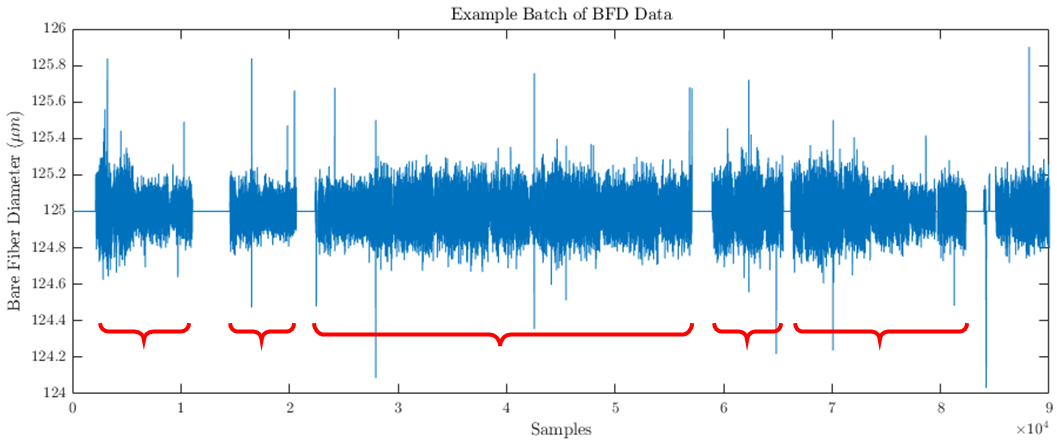
\includegraphics[width=0.8\textwidth]{figures/example_bfd2.png}
    \caption{A portion of the measured BFD signal in a week's data. Each subbatch is labeled with red curly braces.}
    \label{fig:example_bfd}
    
    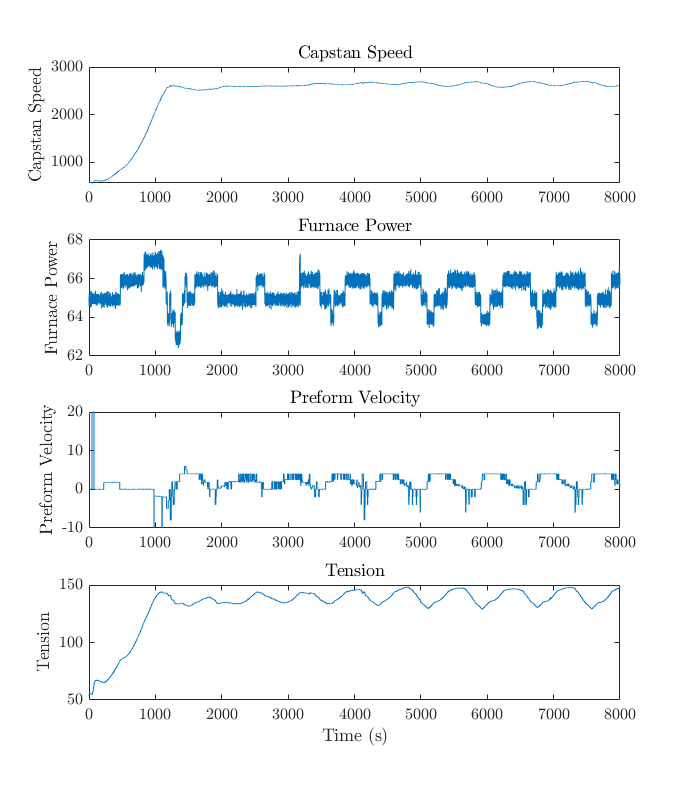
\includegraphics[width=0.85\textwidth]{figures/values.png}
    \caption{An example of input signals to the neural network in a particular subbatch.}
    \label{fig:example_values}
\end{figure}

\begin{figure}[t!]
    \centering
    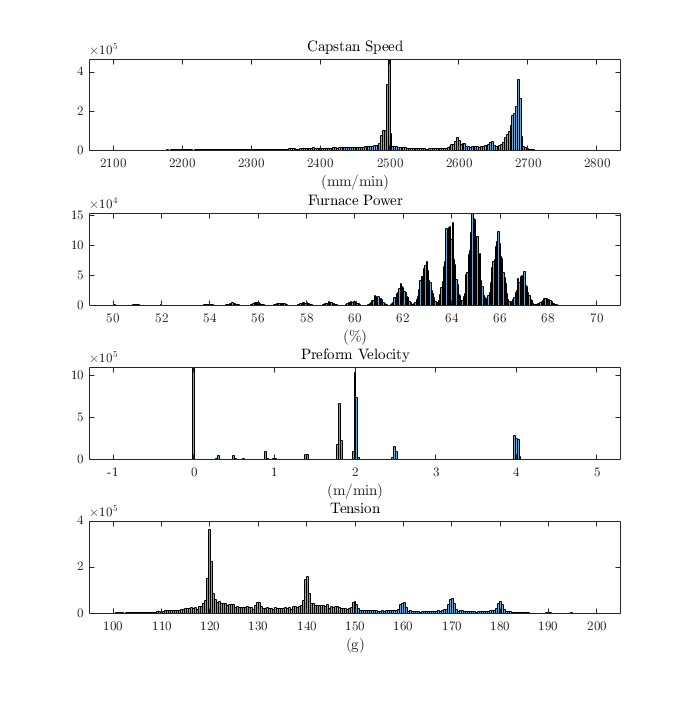
\includegraphics[width=\textwidth]{figures/values_hist.png}
    \caption{Histogram illustrating range of all input signals.}
    \label{fig:values_hist}
\end{figure}

Figure \ref{fig:example_bfd} illustrates a portion of the measured BFD signal in a typical week of production data. Per industrial standards, the nominal BFD is set at 125 microns ($\mu m$) to be compliant with general specifications for optical fiber. However, there are notable breaks in the fiber and perturbations for which the BFD diverges from target value. This is a normal part of the manufacturing process; breaks could occur due to underheating, coating defects, and other irregularities in the preform material \cite{breaks1, breaks2}. Manual intervention is required when this happens; the operator would manually disengage the controller, adjust the tower before re-engaging the controller to bring production back to nominal. 

Upon a closer look at each contiguous region of the BFD, stable production usually results in BFD measurements ranging from 124 to 126 microns. (Refer to Figure \ref{fig:example_bfd}.) In our analysis, we define each week of data as a \emph{batch}. Within a week, each contiguous region of stable production that are greater than 2000 samples is referred to as a \emph{subbatch}, illustrated with red curly braces in Figure \ref{fig:example_bfd}. Each subbatch is limited to a maximum length of 8000 samples to normalize the input size to the neural network. 

The main goal of the machine learning experiments is obtain a dynamical model, in the form of a neural network, that authentically represents the behavior of the aggregate fiber drawing plant. The developed surrogate model could be tested using classical methods (e.g. observing its frequency response) in simulation. Factors that impact the learning of said dynamical model include the neural network architecture, filter lengths, and steady-state range thresholds. We performed experiments investigating the effect of each of these factors on model performance, and from the experimental outcomes, we obtain the best-performing model to be used in a closed-loop simulation. 

\section{Learning Experiments and Explorations} \label{ch:exp:exp}

\subsection{Architecture Experiments} \label{ch:exp:arch}

In setting up the LSTM networks to represent the surrogate model of the plant, the inputs and outputs of the LSTM correspond to those of the black-boxed plant system in the schematics. Namely, the input variables are furnace power, helium tube temperature, capstan speed, and preform velocity; the output variables are the BFD and tension. Refer to the arrows into and out of the red dashed box in Fig. \ref{fig:stl_system_diag}.

We experimented with four different LSTM architecture designs: a single LSTM layer network, a single biLSTM layer network, a 3 side-by-side LSTM layer network, and a 3-layer deep LSTM network. In their architectures, the first layer is a normalization layer in which the inputs are subtracted by the mean and normalized by the standard deviation. It has been demonstrated that normalization of input data usually translates to numerical stability as well as better learning results \cite{normalization1, normalization2}. The first two architectures utilized a 128-neuron LSTM layer followed by a fully connected layer for output. Inspired by the results from \cite{gonzalez}, the side-by-side architecture sent its input to all of its three 128-neuron LSTM layers, concatenated their response, and passed it into a fully connected layer for output. The deep LSTM architecture has three 128-neuron LSTM layers stacked one after another. An illustration depicting these network architectures is shown in Fig. \ref{fig:nn_archs}. 

\begin{figure}[t!]
    \centering
    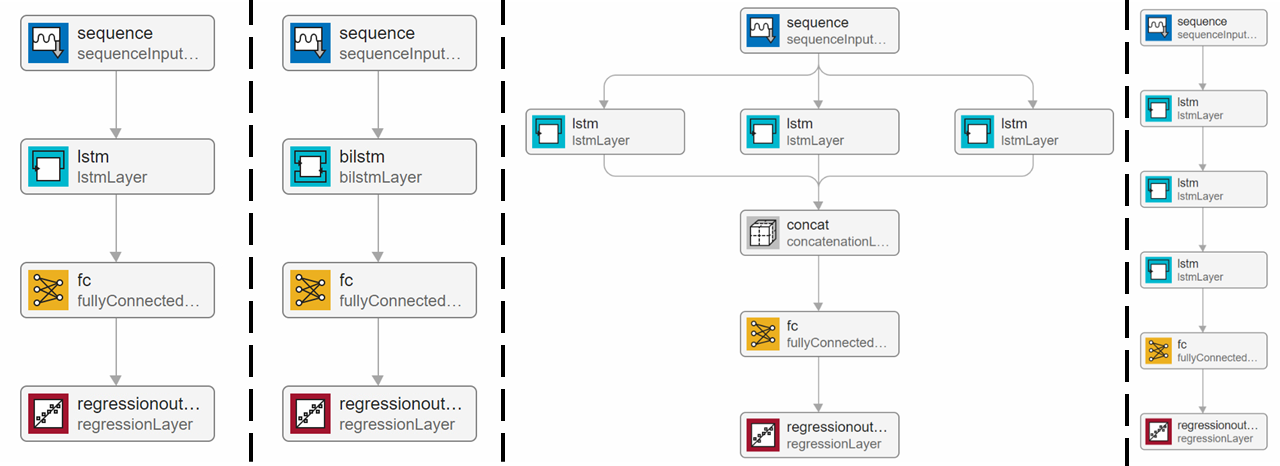
\includegraphics[width=\textwidth]{figures/architectures.png}
    \caption{Four architecture designs experimented in this paper: single layer LSTM, single layer biLSTM, side-by-side LSTM, deep LSTM (from left to right, respectively). }
    \label{fig:nn_archs}
\end{figure}

\begin{figure}[t!]
    \centering
    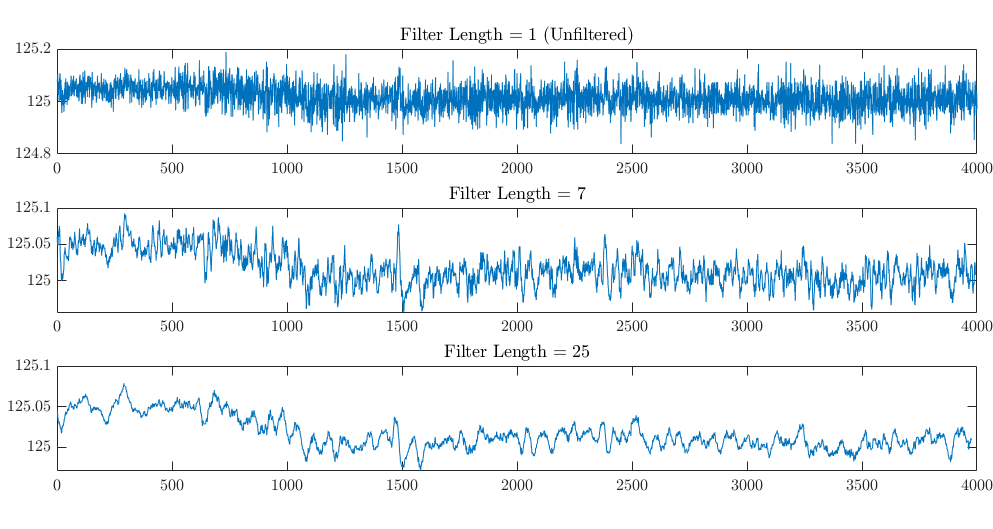
\includegraphics[width=0.99\textwidth]{figures/filter.png}
    \caption{Effect of sliding-window filter on the BFD output.}
    \label{fig:filter}
\end{figure}

\subsection{Filter Lengths on Output}
We implemented low-pass filters of various filter lengths in a sliding window fashion on the output signal. The effect of the sliding-window filter is visualized in Figure \ref{fig:filter}.\footnote{Selected from Week 1, Subbatch 19 in Tower 48 training data.} These experiments serve a two-fold purpose. Firstly, the training data contained a noisy signal for BFD. As a measure to avoid having the neural network train on the noise, the filter suppressed the high-frequency noise in the signal. In addition, we aimed to determine the impact of the filter on the model's ability to capture both low- and high- frequency process dynamics, as well as its generalizability. 

\subsection{Steady State Range Thresholds}
A component of our data pre-processing is selecting the range of values which we define as indicators of steady state behavior. Namely, the range selected is between the low and high BFD thresholds. However, the transient behaviors, which appear after recovering from a break, are essential to include in the model's training data. Refer to Figure \ref{fig:bfd_thresholds} for a comparison between two sets of thresholds. We attempted to widen said thresholds and include more transient behaviors of the plant, so to see the impact of exposing the neural network to more non-steady-state data on the robustness of the surrogate model. 

\begin{figure}[ht]
    \centering
    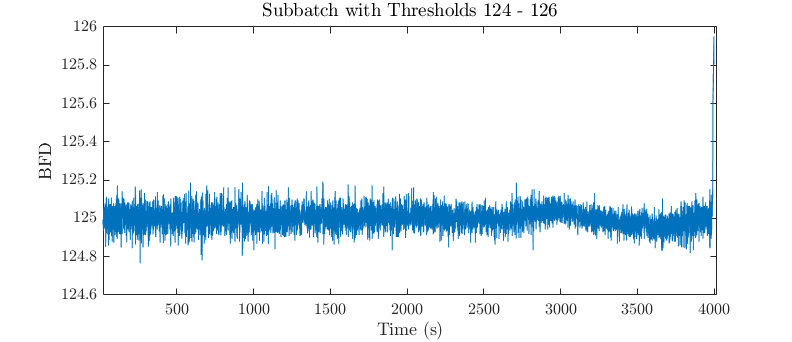
\includegraphics[width=\textwidth]{figures/thres_124126.png}
    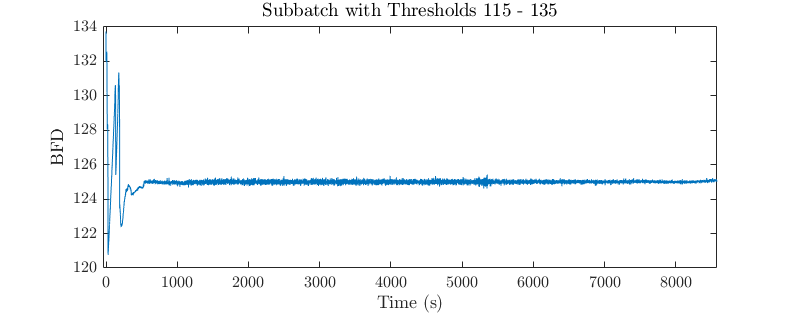
\includegraphics[width=\textwidth]{figures/thres_115135.png}
    \caption{Comparison between two sets of BFD thresholds in data pre-processing. Widened thresholds include more transient dynamics. }
    \label{fig:bfd_thresholds}
\end{figure}

\subsection{Long-Term Drift in Model Parameters}
Mechanical systems, especially those in continuous production, are susceptible to wear and tear over time and seasonal patterns. In developing this surrogate model of the fiber drawing plant, we were interested in whether the model parameters are time-varying in the long term, and by what extent if so. To examine the long-term patterns, we chose the best-performing model architecture from experiments mentioned above, validated it on each week of data, and examine the performance across all weeks. Separately, we also evaluated the performance of each week's model on all other weeks of data. 

\subsection{Model Specificity on Towers}

There were two fiber extrusion tower investigated, namely Tower 48 and Tower 51, with some process differences between the towers. We trained a deep LSTM network for each tower (hereinafter referred to as "Tower 48 model" and "Tower 51 model"), and we were interested in cross-validating the models' ability to predict the BFD output, i.e. using a model trained on one tower's data to predict on the other tower, and vice versa. From that outcome, we were to determine the necessity to separately train different models using production data measured in each tower. \\
\newline
The results of these experiments will be presented in Section \ref{ch:exp:results} below. 

\section{Training} \label{ch:exp:train}

We utilized 14 weeks worth of fiber drawing production data in each experiment. The training and testing datasets were partitioned by a 90:10 split on these data. All training experiments and analyses were performed using MATLAB R2021b. 

The training process involved tuning some hyperparameters to optimize for prediction accuracy. They are listed in Table \ref{tab:hyper_param}, most of which are obtained largely by trial and error. 

% explain init learning rate, learning rate schedules, (EXPLAINED IN CH2) how matlab implements it in drop period,  cite how it's effective

\begin{table}[b!]
    \centering
    \begin{tabular}{c c}
         Name & Value \\ \hline 
         Max epochs & 250\\ 
         Mini-batch size & 16\\ 
         Gradient Threshold & 10 \\ 
         Initial Learning Rate & 0.01 \\
         Learn Rate Drop Period & 100 \\ \hline
    \end{tabular}
    \caption{Hyperparameters for training the surrogate model.}
    \label{tab:hyper_param}
\end{table}

We began by comparing the ability of every architecture to learn and predict on unseen data.
All three architectures were trained for 250 epochs and the model with the lowest seen loss on the testing data was selected as output.
We present the testing losses of each of the architectures below.

\section{Metrics and Results} \label{ch:exp:results}

In evaluating the accuracy of one particular trained model, we used root-mean-square error (RMSE) between the measured BFD and predicted BFD as one of the metrics. However, the values of RMSE were used relatively, i.e. one particular RMSE has little meaning unless compared with RMSEs of other models. When examining the robustness of a surrogate model, we evaluated its performance by running inference on other inputs. All RMSEs are recorded in a \emph{cross-validation matrix} and patterns are observed. In addition, the power spectrum of the predicted dynamics is also evaluated. 

\subsection{Architecture Experiments}

\begin{table}[t!]
    \centering
    \begin{tabular}{r r}
         Architecture & RMSE \\ \hline
         Single Layer LSTM & 0.0817\\
         Single Layer BiLSTM & 0.0818\\
         Side by Side LSTM & 0.0817 \\
         Deep LSTM & 0.0824 \\ \hline
    \end{tabular}
    \caption{The four neural network architectures perform similarly on the RMSE metric. The single layer LSTM and side-by-side LSTM architectures appear to have the lowest RMSE, but have different output waveforms.}
    \label{tab:rmse_error}
\end{table}

The obtained RMSEs after training all four architectures are tabulated in Table \ref{tab:rmse_error}. Although the simple LSTM and side-by-side LSTM architectures got a similarly low RMSE, their output characteristics are very different. Evident in Fig. \ref{fig:prediction}, the single layer LSTM output is much closer to the real signal. The side-by-side LSTM network, however, was unable to accurately model the dynamics of BFD. Instead, it outputs a low-variance signal following the low frequency dynamics of BFD. Therefore, RMSE alone is not a sufficient metric to evaluate the performance of a black-box model; we are also interested in the model's performance as a function of frequency. A visual comparison of the power spectrum revealed that, the prediction agrees with the measured signal to a greater extent on the lower frequency range and the prediction performance slightly degrades at higher frequencies. The deep LSTM architecture performed the best, with its waveform closely following the real signal. It is thus selected as the architecture of choice for the following experiments performed. With the best-performing deep LSTM network, the prediction of tension error is illustrated in Figure \ref{fig:tension}. \footnote{Selected from Subbatch 32 of Tower 48 test data.}

\begin{figure}
    \centering
    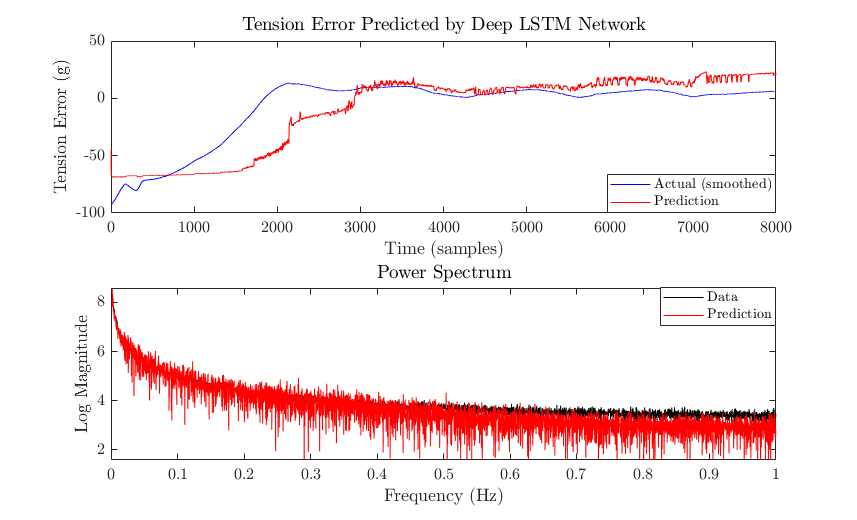
\includegraphics[width=\textwidth]{figures/tension.png}
    \caption{Deep LSTM model performance on predicting tension error. }
    \label{fig:tension}
\end{figure}

This result isn't surprising. Machine learning as a field is inherently experimental; the superior performance of the side-by-side architecture was proven in \cite{gonzalez} using synthetic data, whereas the real production data used in this study are completely different in nature. 

\subsection{Filter Lengths on Output}

% \begin{table}[h]

% \begin{tabular}{l|c c c c}
% \hline
%  & Data, no filter & Data, filter=3 & Data, filter=5 & Data, filter=7 \\ \hline
% Model, no filter    & 7.1883 & 7.9245 & 9.5703 & 11.2197 \\
% Model, filter=3     & 7.6234 & 8.1328 & 9.6085 & 11.1611 \\ 
% Model, filter=5     & 7.9734 & 8.1757 & 9.3822 & 10.7667 \\
% Model, filter=7     & 8.1633 & 8.3432 & 9.3241 & 10.5022 \\ \hline
% \end{tabular}

% \caption{Effect of Filter Lengths on Training Accuracy.}
% \label{tab:filter_len}
% \end{table}

\begin{figure}[h!]
    \centering
    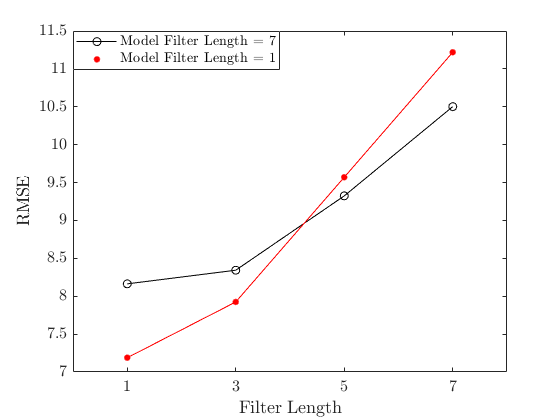
\includegraphics[width=0.75\textwidth]{figures/filter_length.png}
    \caption{Effect of filter length during training on model generalizability.}
    \label{fig:filter_len}
\end{figure}

%From the results from Table \ref{tab:filter_len} and the visualization in Figure \ref{fig:filter_len}, our 
The experiment outcomes shown in Figure \ref{fig:filter_len} suggest that a model trained on the unfiltered data (red curve) performed the best only on unfiltered or lightly filtered data, whereas a model trained on heavily filtered data (black curve) achieved mediocre performance for various filter lengths. With a more aggressive low-pass filter on the training data, the model learned the low-frequency components in all data, which makes it more robust in its prediction. Figure \ref{fig:filter_len_time_series} provides a comparison of model performances between both types of models in time- and frequency- domain.\footnote{Selected from Subbatches 43 and 243 of Tower 48 data, respectively.} The model trained on unfiltered data was able to predict the high-frequency dynamics in the BFD, whereas the one trained on filtered data only captured the low-frequency content in the BFD signal. 

\begin{figure}
    \centering
    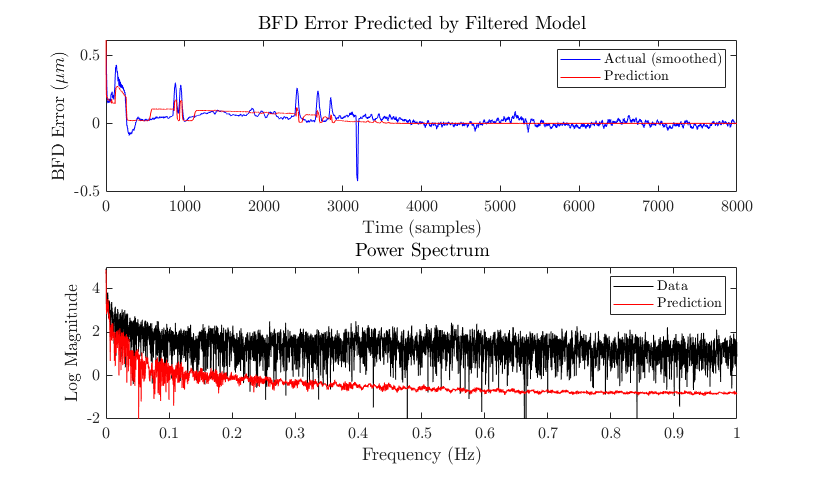
\includegraphics[width=\textwidth]{figures/filter_len_filtered.png}
    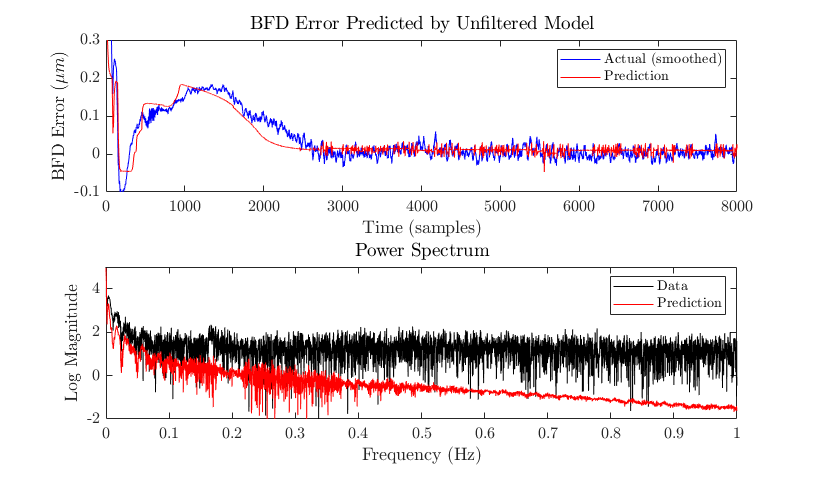
\includegraphics[width=\textwidth]{figures/filter_len_unfiltered.png}
    \caption{Comparison of model performances on BFD prediction using models trained on filtered (filter length of 7) and unfiltered (filter length of 1) data. The unfiltered training data give the model ability to recognize high-frequency dynamics.}
    \label{fig:filter_len_time_series}
\end{figure}

\begin{figure*}[ht!]
    \centering
    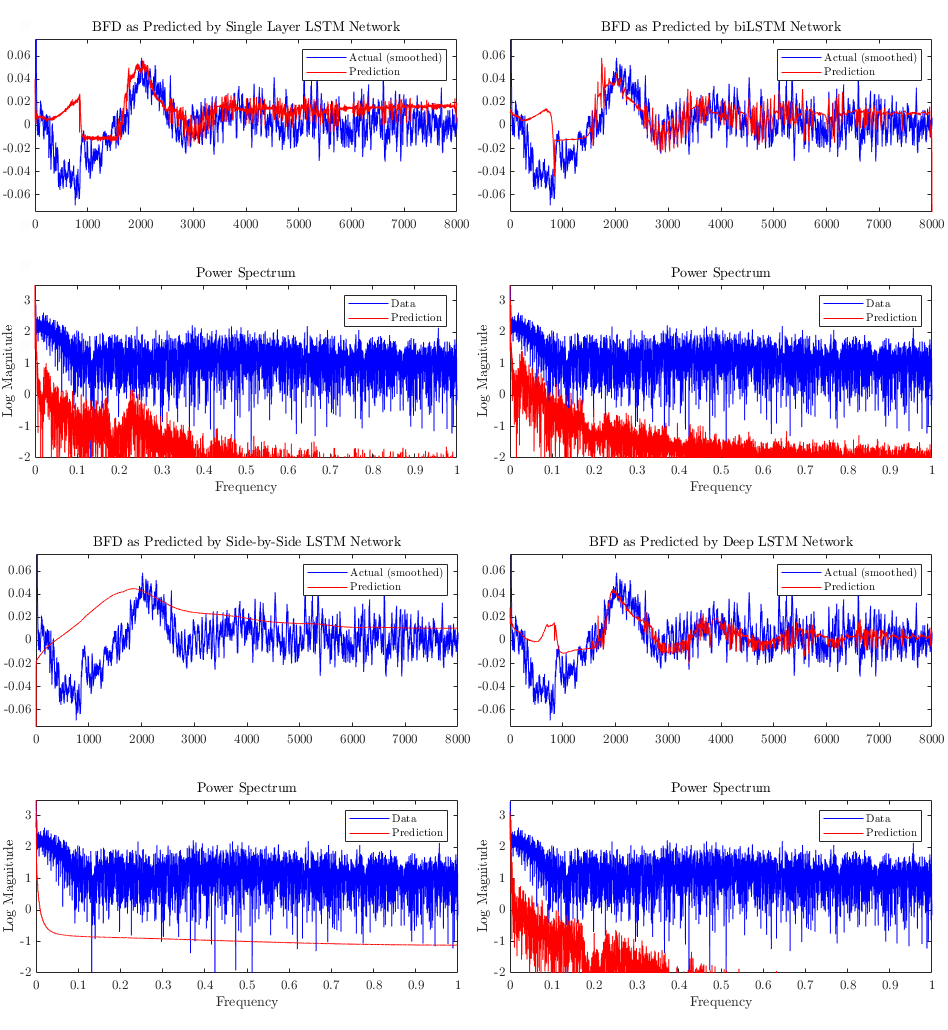
\includegraphics[width=\textwidth]{figures/combine_images.png}
    \caption{Mean-removed BFD as predicted by four network architectures.}
    \label{fig:prediction}
\end{figure*}

\subsection{Steady State Range Thresholds}

\begin{table}[ht!]
    \centering
        \begin{tabular}{|c|c|c|}
            \hline
            BFD Thresholds & RMSE & \makecell{RMSE on \\ 124-126 Data} \\ \hline
            124 - 126 & 0.0852 & 0.094\\
            123 - 127 & 0.0772 & 0.099\\
            122 - 128 & 0.0998 & 0.105\\
            121 - 129 & 0.1048 & 0.112\\
            120 - 130 & 0.1421 & 0.129\\
            119 - 131 & 0.1838 & 0.139\\
            118 - 132 & 0.2095 & 0.177\\
            117 - 133 & 0.2353 & 0.123\\
            116 - 134 & 0.3548 & 0.128\\
            115 - 135 & 0.2956 & 0.173\\ \hline
        \end{tabular}
        \caption{Effect of transient dynamics on RMSE and on model performance within region of interest.}
        \label{tab:thresholds}
\end{table}

Including more transient dynamics apparently compromises the machine learning model's ability to predict. This is represented by an increasing RMSE score across models when trained on data with varying amounts of transient dynamics. As shown in Table \ref{tab:thresholds}, the model trained on the least amount of transient dynamics was able to achieve the lowest RMSE, while all other models, trained on data with higher variance on the BFD, performed worse than the baseline. The modeling accuracy also did not benefit from including more transient dynamics on our data range of interest, 124 to 126 microns of BFD. This can be seen also in Table \ref{tab:thresholds}, where the model with the lowest RMSE on the data range of 124 to 126 is the model trained on said data range. 

\subsection{Long-Term Drift in Model Parameters}

\begin{figure}[ht!]
    \centering
    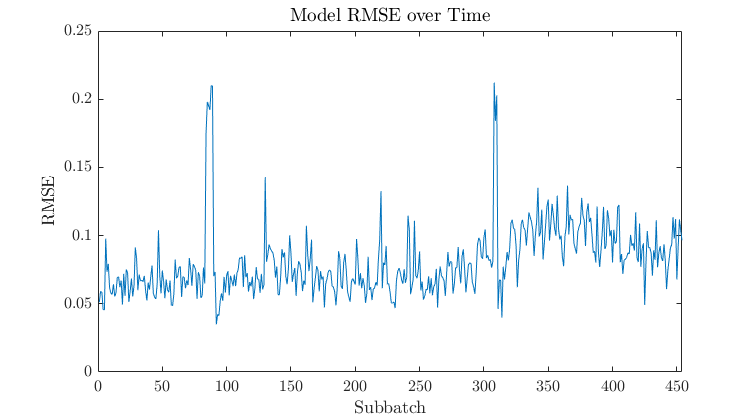
\includegraphics[width=\textwidth]{figures/drift.png}
    \caption{RMSE of the best-performing surrogate model over time.}
    \label{fig:drift}
\end{figure}

The deep LSTM neural network was shown to be the best-performing model in Section \ref{ch:exp:arch}. It was therefore chosen to perform inference on system output, namely the predicted BFD signal. The RMSEs of all subbatches of data (chronologically) are plotted in Figure \ref{fig:drift}. Note the few spikes in the RMSE; they correspond to the subbatches of shorter lengths than most other ones. This is because, to a certain extent, a higher data volume during the training of a model expands the convex hull of the training data and reduces the error in validation, enabling the model to generalize better. Future iterations of this study could normalize the subbatch length or the weigh the metric of RMSEs for comparable results. A similar effect of the subbatch length is also shown in the result of validating each week's model on all other weeks of data, particularly in Models 6 and 10 of Table \ref{tab:drift}.

\begin{table}[t!]
    \centering
    \resizebox{\textwidth}{!}{
    \begin{tabular}{c|c|c|c|c|c|c|c|c|c|c|c|c|c|c}
 & Week 1 & Week 2 & Week 3 & Week 4 & Week 5 & Week 6 & Week 7 & Week 8 & Week 9 & Week 10 & Week 11 & Week 12 & Week 13 & Week 14 \\ \hline
Model 1 & 2078 & 2635 & 250576 & 3056 & 2673 & 2049 & 2950 & 2101 & 2890 & 2811 & 3303 & 4858 & 3768 & 2887 \\
Model 2 & 2443 & 2527 & 18817 & 2718 & 2613 & 2327 & 2591 & 2383 & 2861 & 2514 & 3073 & 7939 & 11649 & 2786\\
Model 3 & 2333 & 6196 & 2064 & 3243 & 3066 & 2921 & 2599 & 2093 & 4417 & 2925 & 3854 & 3795 & 334879 & 3019\\
Model 4 & 2345 & 4691 & 2677 & 2414 & 2793 & 2386 & 8001 & 2473 & 2645 & 7739 & 8041 & 4616 & 5201 & 2522\\
Model 5 & 2924 & 4070 & 2698 & 3525 & 2678 & 3058 & 3754 & 2553 & 4424 & 3263 & 4329 & 4280 & 4376 & 3688\\
Model 6 & 4097 & 8823 & 1637684 & 12679 & 3399 & 2120 & 19559 & 355447 & 5007 & 15084 & 460871 & 2007124 & 6387426 & 2821549\\
Model 7 & 2743 & 3215 & 3003 & 2644 & 3014 & 2812 & 2357 & 2753 & 2881 & 2608 & 6908 & 3117 & 5141 & 2598\\
Model 8 & 6435 & 7538 & 25778 & 6158 & 3669 & 4607 & 4037 & 2327 & 7739 & 3364 & 9187 & 21440 & 7060 & 9731\\
Model 9 & 16709 & 10917 & 58923 & 3707 & 4242 & 3006 & 14607 & 54707 & 2588 & 14688 & 36115 & 89016 & 9550 & 3761\\
Model 10 & 55431 & 126472 & 76508 & 9518 & 26893 & 13851 & 2280 & 2006 & 61139 & 2134 & 105801 & 173357 & 57141 & 78577\\
Model 11 & 2313 & 2448 & 2365 & 2233 & 2344 & 2349 & 2269 & 2268 & 2478 & 2175 & 2665 & 2622 & 2453 & 2449\\
Model 12 & 2036 & 2559 & 2152 & 2348 & 2081 & 2320 & 2898 & 1826 & 2792 & 2824 & 2807 & 2526 & 2631 & 2320\\
Model 13 & 1814 & 2083 & 3598 & 2081 & 1862 & 1967 & 3063 & 1745 & 2241 & 2086 & 5645 & 8090 & 2247 & 2438\\
Model 14 & 2290 & 2847 & 2309 & 2493 & 2483 & 2603 & 3244 & 2095 & 2871 & 3374 & 3025 & 2799 & 2936 & 2408\\ \hline
    \end{tabular}
    }
    \caption{Cross-validation matrix of each week's trained model validating on all other weeks of data from Tower 48. }
    \label{tab:drift}
\end{table}

\subsection{Model Specificity on Towers}

\begin{figure}[ht!]
    \centering
    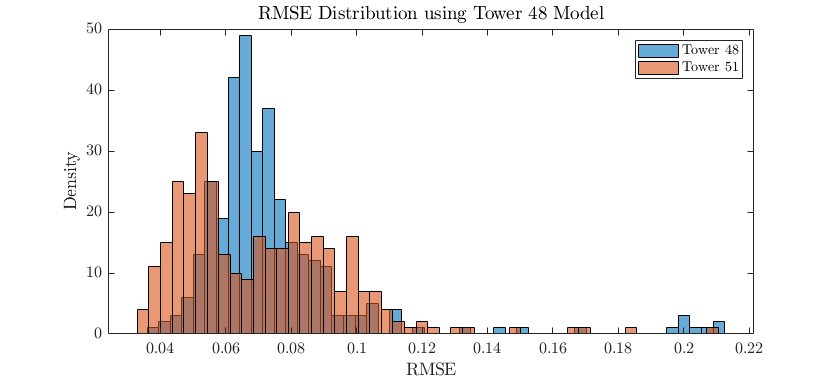
\includegraphics[width=\textwidth]{figures/model48_errors.png}
    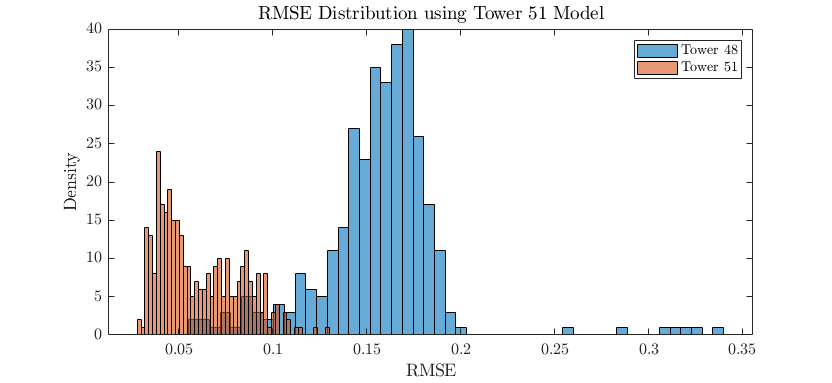
\includegraphics[width=\textwidth]{figures/model51_errors.png}
    \caption{Cross-validation of Tower 48 and Tower 51 models on each other's datasets.}
    \label{fig:tower_rmse}
\end{figure}

Figure \ref{fig:tower_rmse} offers a comparison of the RMSE distributions using the Tower 48 model and Tower 51 model, respectively. By running inference using the Tower 48 model on production data from each tower, we discovered that the RMSEs are similar in range, although the predictions on Tower 48 data are more consistent as compared to Tower 51 data, as shown by the lower variance in the histogram. The Tower 51 model demonstrated better performance on Tower 51 data only, and the Tower 48 model is more generalizable to Tower 51. 

\section{Discussion}

This chapter discussed an approach to model the optical fiber drawing process using LSTM networks. Using a deep LSTM neural network, we investigated the effects of filtering and inclusion of transient dynamics on model generalizability. Further fine-tuning of parameters could potentially lead to marginally better results, but a few limitations of this approach should be addressed. 

Firstly, each subbatch of data has a high variance due to variations in the production environment. The LSTM models may have slightly degraded performance when the validation data has amplitudes beyond the range seen within the training set \cite{lstm_amplitude}.

The process dynamics of fiber extrusion inherently does not have long-term memory. Instead, it is governed by a complicated set of governing differential equations that depends on the inputs, its current state, and finite-order differentials. It could be the case that the LSTM is erroneously finding long-term dependencies in the evolution of the BFD signal that do not actually exist. Further, memorizing past trajectories without learning the underlying dynamical structure has been proven ineffective in machine learning tasks involving nonlinear systems \cite{fu_et_al}. To address these problems, recommendations for further studies, which involve embedding the physical models into neural network models, are provided later in Section \ref{ch:concl:future_work}.
\chapter{System Identification} \label{ch:sysid}

The second aspect of this thesis involves modeling the existing controllers operating the fiber drawing plant. Given limited information about the controllers (e.g. their order and sampling time), a time-series statistical analysis approach is used to model each controller and simulate outputs. The theory behind time-series system identification is briefly reviewed in Section \ref{ch:sysid:theory}. Section \ref{ch:sysid:proc} describes the methods and analyses involved in identifying and validating models, as applied to our optical fiber extrusion system. Lastly, the process of identifying the bare fiber diameter controller is presented in Section \ref{ch:sysid:case} as a case study. All analyses were performed using MATLAB R2021b. 

\section{Theory of Data-Based Models} \label{ch:sysid:theory} 

As discussed in Section \ref{ch:ml:relation}, the dynamics of a discrete nonlinear system is a function of the system's past states and inputs, up to some number of timesteps. (Refer to Equation \ref{eqn:nonlinear_discrete}.) Aside from RNNs, there are also data-based models well-suited for time-series prediction and identifying controllers. \cite{armax1, armax2} If given a sufficient amount of input-output data of a system, a model can be developed solely on those data while abstracting away from the equations of motion and the underlying physics. This is the essence behind black-box system identification. It allows for modeling dynamical systems not easily derived from first principles. 

\begin{figure}[t!]
    \begin{center}
        \tikzstyle{ann} = [above, text width=2.5em]
        \def\edgedist{3}
        \begin{tikzpicture}
                % draw rectangle node
                \node[draw,
                    minimum width=4cm,
                    minimum height=2cm] (sys) at (0,0) {Black-box System};
                \node[draw=white,
                    minimum width=0cm,
                    minimum height=0cm] (empty) at (-5,0) {};
                % Draw edges
                \draw [->] (sys.east) -- node [ann] {output} + (\edgedist,0);
                \draw [->] (empty.east) -- (sys.west) node[midway,above] {input};
        \end{tikzpicture}
    \end{center}
    \caption{Black-box view of system identification.}
    \label{fig:blackbox}
\end{figure}

System identification has been a well-studied topic in literature. Black-box models have been developed for damping controllers in power grids \cite{smartgrid}, model predictive controllers for car-following \cite{car_following}, static heat flow estimation \cite{static_heat_flow}, just to name a few. It is a widely used and powerful technique to model systems from measured, and often noisy, data. An accurate model of the system is helpful for predicting system outputs from given inputs; such input-output correlations, in turn, guides the design of controllers that enable the system to reach desired performance.

\begin{figure}[b!]
    \centering
    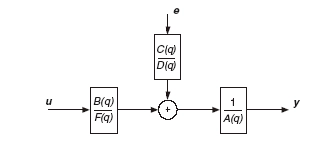
\includegraphics{figures/sys_general.png}
    \caption{General linear model structure for the system identification problem \cite{ni}.}
    \label{fig:sys_general}
\end{figure}

The time-series system identification problem can be posed as follows. Figure \ref{fig:sys_general} illustrates the general discrete-time linear model for a Single-Input, Single-Output (SISO) process. It can be described by the difference equation in Equation \ref{eqn:sysid_general}. 
\begin{equation}
    \label{eqn:sysid_general}
    A(q) y(t) = \frac{B(q)}{F(q)} u(t) + \frac{C(q)}{D(q)} e(t)
\end{equation}
where $u(t)$ is the system input and $y(t)$ the system output. $e(t)$ is the noise signal entering the system and is usually assumed to be white noise. $q$ denotes the \emph{time-shift operator} which, when applied to a signal, advances the signal one timestep ahead. Inversely, applying $q^{-1}$ to a signal shifts the signal backwards by one timestep. Mathematically, 
\begin{equation}
    \label{eqn:def_q}
    \begin{split}
        qu(t) & = u(t+1) \\
        q^{-1}u(t) & = u(t-1)
    \end{split}
\end{equation}

As $A$, $B$, $C$, $D$, and $F$ are defined as polynomials of $q^{-1}$, the system output $y(t)$ at the current timestep is predicted as a function of data from the past timestep(s). Implicit in these model architectures is the assumption of \emph{causality} — the property that outputs depend on the past and current inputs but not future inputs. Specifically, 
\begin{equation}
    \begin{split}
        A(q) &= 1 + a_1 q^{-1} + ... + a_{n_a} q^{-n_a}\\
        B(q) &= b_1 + b_2 q^{-1} + ... +b_{n_b} q^{-n_b+1}\\
        C(q) &= 1 + c_1 q^{-1} + ... + c_{n_c} q^{-n_c}\\
        D(q) &= 1 + d_1 q^{-1} + ... + d_{n_d} q^{-n_d}\\
        F(q) &= 1 + f_1 q^{-1} + ... + f_{n_f} q^{-n_f}
    \end{split}
\end{equation}

In this work, two specific models of the generalized architecture described above are explored: the Output-Error (OE) model, and the AutoRegressive Moving-Average model with eXogenous inputs (ARMAX). The theory behind their architectures is treated in detail in the following subsections. 

\subsection{OE Model}

\begin{figure}[h]
    \centering
    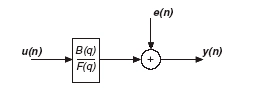
\includegraphics{figures/oe.png}
    \caption{Diagram of the OE model \cite{ni}.}
    \label{fig:oe}
\end{figure}

Figure \ref{fig:oe} illustrates the architecture of the OE model. Its model structure is given by

\begin{equation}
    \label{eqn:oe}
     y(t) = \frac{B(q^{-1})}{F(q^{-1})} u(t-n_k) + e(t)
\end{equation}
where $n_k$ is known as the \emph{input delay}\footnote{Also known as \emph{transport delay} or \emph{dead time}.} of the system, which is the number of input samples that occur before the outputs are affected. The OE model structure describes the system dynamics separately from the noise signal. The polynomial acting upon the noise signal $e(t)$ is unity, which means that the noise entering the system is modeled to be zero-mean white noise, and no other parameters are used to characterize the disturbance. 

\subsection{ARMAX Model}

\begin{figure}[h]
    \centering
    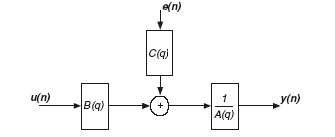
\includegraphics{figures/armax.png}
    \caption{Diagram of the ARMAX model \cite{ni}.}
    \label{fig:armax}
\end{figure}

A diagram of the ARMAX model is depicted in Figure \ref{fig:armax}. Its input-output relation is given by
\begin{equation}
    \label{eqn:armax}
    A(q^{-1}) y(t) = {B(q^{-1})} u(t-n_k) + {C(q^{-1})} e(t)
\end{equation}
where all variables are similarly defined as before. The ARMAX model is no more than the specific case of the general system in Equation \ref{eqn:sysid_general}, with $D$ and $F$ polynomials set to unity. Unlike the OE model, the ARMAX model integrates the disturbance dynamics together with the system dynamics. It is particularly useful due to its assumption that there are prominent disturbances entering at the input and propagating through the system dynamics. The error dynamics is also parametrized by $C(q)$, which indicates that the noise is assumed to be colored. 

\subsection{Implementation in MATLAB}

The parameter estimation process was implemented in MATLAB with its System Identification Toolbox. Given the input-output data of a system (in the form of an \texttt{iddata} object) and specified orders of each polynomial, the toolbox provides functions, such as \texttt{oe(data, orders)} and \texttt{armax(data, orders)}, that perform the model fitting and return a representation of the system as an \texttt{idpoly} object (the MATLAB representation of the generalized system in Figure \ref{fig:sys_general}). 

The identified parameters are the result of an iterative search algorithm, introduced in a paper by Wills et al. \cite{iter_sysid_wills}. The algorithm poses a least squares optimization problem in which the prediction error, i.e. the error between simulated output from the prediction and measured output from the data, is minimized. As proven by Ljung (1999) \cite{ljung1999system}, the general model described by Equation \ref{eqn:sysid_general} is linear in its parameters, therefore it is appropriate to pose the parameter identification problem in the general model as a multi-stage least square problem. MATLAB also has built-in functions to validate identified models, using the normalized root mean square error (NRMSE) as the figure of merit. Namely, for a measured output $y$ with mean $\Bar{y}$ and a prediction output $\hat{y}$, the percentage of accuracy is calculated as, 

\begin{equation}
    \label{eqn:sysid_fit}
    \text{fit} = \left(1-\frac{\left\lVert y-\hat{y}\right\rVert}{\left\lVert y-\Bar{y}\right\rVert}\right) \times 100 \%
\end{equation}

The iterations terminate when the specified maximum number of iterations is reached or the accuracy increment is lower than the specified tolerance. %The validation process for this work will be discussed in full detail in Section \ref{ch:sysid:proc:val}.

\section{System Identification Procedures} \label{ch:sysid:proc}

\begin{figure}[ht!]
    \centering
    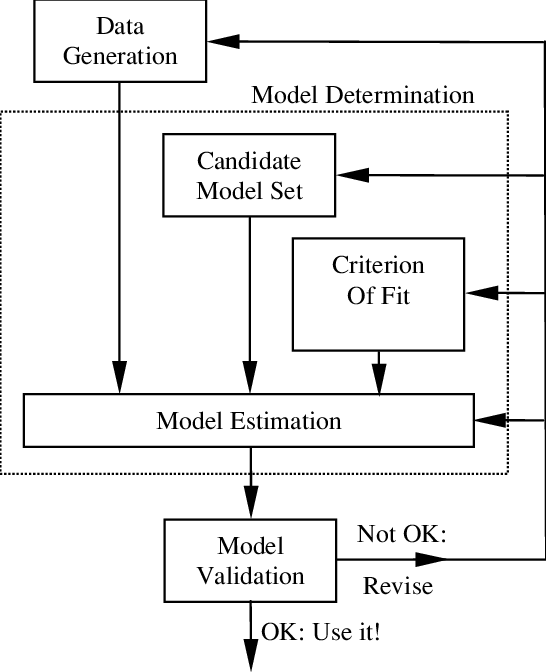
\includegraphics[width=0.6\textwidth]{figures/sysid_pipeline.png}
    \caption{Diagram of the system identification pipeline \cite{sysid_pipeline}.}
    \label{fig:sysid_pipeline}
\end{figure}

Introduced by Ljung \cite{ljung1999system}, the system identification method is an iterative process to identify a model with some \emph{a priori} knowledge of the system. In general, given the measured input-output data of a system, the task of system identification can be divided into subproblems as follows: 

\begin{enumerate}
    \item Design and perform experiments to acquire the necessary input-output data 
    \item Specify a proper model structure or a set of candidate model structures 
    \item Select appropriate model orders in the chosen structure(s) based on the principle of parsimony 
    \item Specify a criterion of fit with which the models are evaluated
    \item Identify the model parameters based on the criterion of fit
    \item Validate the model, examine its properties, and simulate system output
    \item If necessary, revisit any of the steps above and iterate forwards to refine the identified system parameters
\end{enumerate}

The following subsections present the details of this process as applied to the controllers in the fiber drawing system. 

\subsection{Model Order Bounds} \label{ch:sysid:proc:order}

Given the potential candidates for model structures, the objective of system identification is to identify the simplest, interpretable model that provides the best fit to the collected data. Especially for controller design, an underestimate of the orders would result in a biased model, whereas an overly high order model would be less reliable, computationally expensive to implement, and would lose its robustness to disturbances. Thus, the order selection process is usually guided by the \emph{principle of parsimony}, which states that the simplest model that can explain the data is to be preferred. In this work, this principle puts preference on an identified system with the lowest maximum order that satisfies the goodness criteria. 

A reasonable estimate of the range of the system's model order can be drawn from first principles of the physical  system. In this work, the systems in question are bare fiber diameter controller and the tension controller within the optical fiber drawing tower. % TODO: submit that paper and cite myself here
Given limited \emph{a priori} knowledge about the system, namely that the controllers in the tower are implemented as PID controllers, one can begin with analytical equations and develop a first-principles model relating the input to the output. 

\begin{figure}[h!]
    \centering
    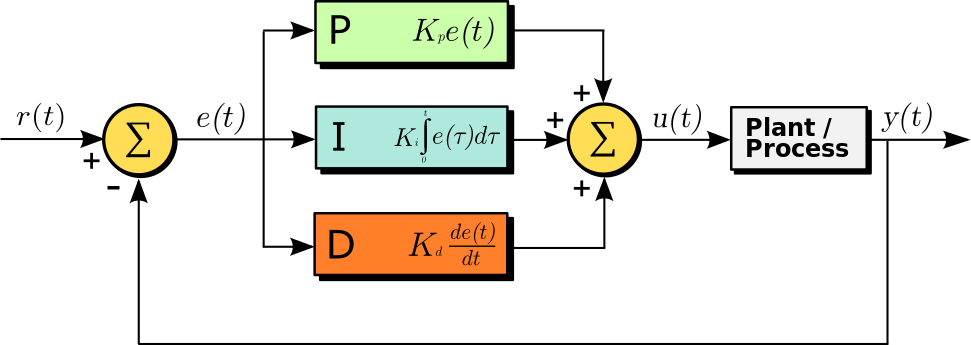
\includegraphics[width=0.8\textwidth]{figures/pid.png}
    \caption{Block diagram of a PID controller in a feedback loop \cite{pid}.}
    \label{fig:pid}
\end{figure}

The internal schematic of a typical PID controller is shown in Figure \ref{fig:pid}. Let $e(t) = r(t) - y(t)$ be the input signal to the PID controller, and is defined as the deviation of the plant output $y(t)$ from the desired reference signal $r(t)$ that the controller aims to follow. Let $u(t)$ be the control effort, the output of the controller. The control law of a PID controller, expressed in the time domain, is shown in Equation \eqref{eqn:pid}. 

\begin{equation}
    \label{eqn:pid}
    \frac{u(t)}{e(t)} = K_P e(t) + K_I\int_0^T e(t) dt + K_D \frac{d}{dt} e(t)
\end{equation}
where $K_P$, $K_I$, and $K_D$ are the proportional, integral, and derivative gains respectively. 

Let's examine the rate of change in the control effort $u(t)$ in Equation \eqref{eqn:pid_dt}. 

\begin{equation}
    \label{eqn:pid_dt}
    \frac{du}{dt} = K_P \frac{d}{dt} e(t) + K_I e(t) + K_D \frac{d^2}{dt^2} e(t)
\end{equation}

In real-world machinery, derivatives are calculated or approximated by taking the finite difference \cite{finite_diff} between time steps. Thus, Equation \eqref{eqn:pid_dt} can be written as 
\begin{equation}
    \label{eqn:pid_fd}
        \frac{u[n]-u[n-1]}{\Delta t} 
         = K_P \frac{e[n]-e[n-1]}{\Delta t} + K_I e[n] + K_D \frac{e[n]-2e[n-1]+e[n-2]}{\Delta t}
\end{equation}
where $\Delta t$ is the sampling time between discrete measurements. 

To reformulate the above relationship with variables used in Section \ref{ch:sysid:theory} and other series analysis literature, we express the above equation in terms of the time-shift operator $q$ (defined in Equation \ref{eqn:def_q}), 
\begin{equation}
    u-q^{-1}u = K_P e (1-q^{-1}) + K_I e \Delta t + K_D e (1-2q^{-1}+q^{-2})
\end{equation}

Rearranging further, we obtain the transfer function of the PID controller as
\begin{equation}
    G(q) = \frac{u(q)}{e(q)} = \frac{K_P (1-q^{-1}) + K_I \Delta t + K_D (1-q^{-1})^2}{1-q^{-1}}
\end{equation}

\begin{equation}
    G(q) = \frac{(K_P + K_D + K_I\Delta t) - (K_P-2K_D) q^{-1} + K_D q^{-2}}{1-q^{-1}}
\end{equation}

This suggests that a PID controller is at least second order in nature. 

In addition, due to the noisy nature of the measured data (illustrated later in Section \ref{ch:sysid:case}), a low-pass filter of some sort is warranted for controller stability. Such filters introduce at least one order in the system. There may also be unmodeled dynamics in the system that is not captured in this analysis, which, in turn, translates to higher order required for a reasonable fit in system identification. Therefore, we have established a third-order lower bound for the identified model. 

\subsection{The Grid Search} \label{ch:sysid:proc:grid}

For each subbatch (defined in Section \ref{ch:exp:data}), a grid search is implemented to select the model orders. The problem is posed as follows. Consider the OE architecture. Let $\mathcal{S}_{OE} \subseteq \mathbb{N}^3$ denote the parameter search space to be iterated through. The maximum order $N_{max}$ is chosen to be the upper limit of the model order in the search space; in this study it is set to be $10$. $K_{max}$, the upper bound of $n_k$, is set to be $4$. Furthermore, with the lower bound of the order determined above, the goal of the grid search is to select an OE model with orders $[n_a, n_b, n_k]$ where

\begin{equation*}
    (n_a, n_b, n_k)\in \mathcal{S}_{OE} = [1, N_{max}]^2 \times [1, K_{max}] \text{\space\space s.t. } \max(n_a, n_b) \geqslant 3
    \label{eqn:oe_bounds}
\end{equation*}

Additionally, the criteria of fit is enumerated below. A selected candidate OE model should: 

\begin{enumerate}
    \item Perform a reasonable fit to a majority of the subbatches\footnote{A reasonable fit is quantified by a minimum percentage accuracy, here set to be 50\%, as calculated using Equation \ref{eqn:sysid_fit}.\label{ftn:good}}
    \item Attain a satisfactory average accuracy across subbatches of good fit\footnote{Some subbatches of data were discarded due to an impossible fit caused by measurement errors from operator interruption.}
    \item Be characterized by polynomials of low orders per the principle of parsimony discussed in Section \ref{ch:sysid:proc:order}.
\end{enumerate}

Once a set of candidate model orders $[n_a, n_b, n_k]$ are identified, engineering decision is involved to choose a model that balances the three objectives above. The pseudocode summarizing this process is presented in Algorithm \ref{alg:grid_search_oe}. The grid search process for ARMAX is similar; the search space $\mathcal{S}_{ARMAX} \subseteq \mathbb{N}^4$ is iterated through, with the same lower and upper bounds determined above, generating candidate models with orders $[n_a, n_b, n_c, n_k]$ where
\begin{equation*}
    % (\texttt{na}, \texttt{nb}, \texttt{nc})\in \mathcal{S} = [1, N_{max}]^3 \text{\space\space s.t. } \max(\texttt{na}, \texttt{nb}, \texttt{nc}) > 3
    (n_a, n_b, n_c, n_k)\in \mathcal{S}_{ARMAX} = [1, N_{max}]^3 \times [1, K_{max}] \text{\space\space s.t. } \max(n_a, n_b) \geqslant 3
    \label{eqn:armax_bounds}
\end{equation*}

As shown in Algorithm \ref{alg:grid_search_oe}, during the grid search process, the accuracy percentages for all orders for all subbatches are stored for comparison purposes, in a table in which each row is a subbatch and each column is a combination of model orders attempted for the fit. A final model is then selected among the best-performing candidate models, after comparing their number of subbatches with reasonable fits and average accuracies. 

% \begin{algorithm}[p]
%     \label{alg:grid_search_oe}  
%     \DontPrintSemicolon
%     \caption{Grid Search for OE Model Orders.}
%     \KwData{$F$ = A list of files each containing many subbatches of fiber production data within a week.}
%     \KwResult{$M$ = A 2D matrix of fit percentages for all subbatches for all orders.}
%     % \For{each file $f \in F$}{
%     %     \For{each subbatch in $f$}{
%     %         \texttt{iddata\_obj} = \texttt{iddata(capstan\_speed, bfd\_error, sampling\_time)}\;
%     \For{na \in [1, N_{max}]}{
%         \For{nb \in [1, N_{max}]}{
%             \If{\textbf{not } na<3 and nb < 3}{
%                 \texttt{sys\_kd} = \texttt{oe(iddata\_obj, [na, nb, 3])}\;
%                 \texttt{fit\_percentage} = \texttt{compare(iddata\_obj, sys\_kd)}\;
%                 \If{$50 \leq fit\_percentage \leq 100$}{
%                     Store fit\_percentage in $M$\;
%                 }
%             }
%         }
%     }
%     %     }
%     % }
% \end{algorithm}

% % REVISE TO USE ALGORITHM2E PACKAGE... LOOKS NICER

\begin{algorithm}[t]
    \KwData{$F$ = A list of files each containing many subbatches of fiber production data within a week.}
    \KwResult{$M$ = A 2D matrix of fit percentages for all subbatches for all orders.}
    \begin{algorithmic}
        \caption{Grid Search for OE Model Orders.}
        \label{alg:grid_search_oe}
        \FOR{each file $f \in F$}{
            \FOR{each subbatch $\in f$}{
            \STATE \texttt{iddata\_obj} = \texttt{iddata(capstan\_speed, bfd\_error, sampling\_time)}\;
                \FOR{$n_a \in [1, N_{max}]$}{
                    \FOR{$n_b \in [1, N_{max}]$}{
                        \FOR{$n_k \in [1, K_{max}]$}{
                            \IF{$\textbf{not } n_a<3 \And n_b < 3$}{
                                \STATE \texttt{sys\_kd = oe(iddata\_obj, [na, nb, 3])}\;
                                \STATE \texttt{fit\_percentage} = \texttt{compare(iddata\_obj, sys\_kd)}\;
                                \IF{$50 \leqslant \texttt{fit\_percentage} \leqslant 100$}{
                                    \STATE Store \texttt{fit\_percentage} in $M$\;
                                } \ENDIF
                            } \ENDIF
                        }\ENDFOR
                    } \ENDFOR
                }\ENDFOR
            } \ENDFOR
        } \ENDFOR
    \end{algorithmic}
\end{algorithm}

\subsection{Model Validation} \label{ch:sysid:proc:val}

\subsubsection{Frequency-Domain Analysis}

Besides comparing the measured output with predicted output signals in the time domain using Equation \ref{eqn:sysid_fit}, the power spectrum of the output signals and the frequency-domain properties of the control loop should be examined when validating the identified model. The power spectrum of the system output should be compared to that of the predicted output. The prediction should not only capture the low-frequency trends in the output but also agrees reasonably in the high-frequency regime. It is important to identify the frequency ranges in which the prediction performs well and ones in which the model's reliability degrades. These characteristics cannot be distinguished by inspecting the time-domain signals alone. 

\subsubsection{Residual Analysis}

The residual signal can be obtained by subtracting the measured output from the predicted output. It is a function of the model structure, quality of data, and nonlinearities in the system. An ideal system model would have a white noise residual signal \cite{ljung_ideal_white}, although this is practically difficult to achieve. \cite{nasa_white_residual} The autocorrelation of the residual is used to visualize the whiteness of the signal. By the definition of whiteness, the signal is a sequence of uncorrelated random variables. Therefore, an ideal residual signal should have an autocorrelation with a peak at zero lag, and nearly zero values (i.e. within specified confidence intervals) everywhere else. %Figure \ref{fig:nasa_xorr} depicts an example of such autocorrelation graph of a residual signal, with which one can validate an identified model. 

% \begin{figure}
%     \centering
%     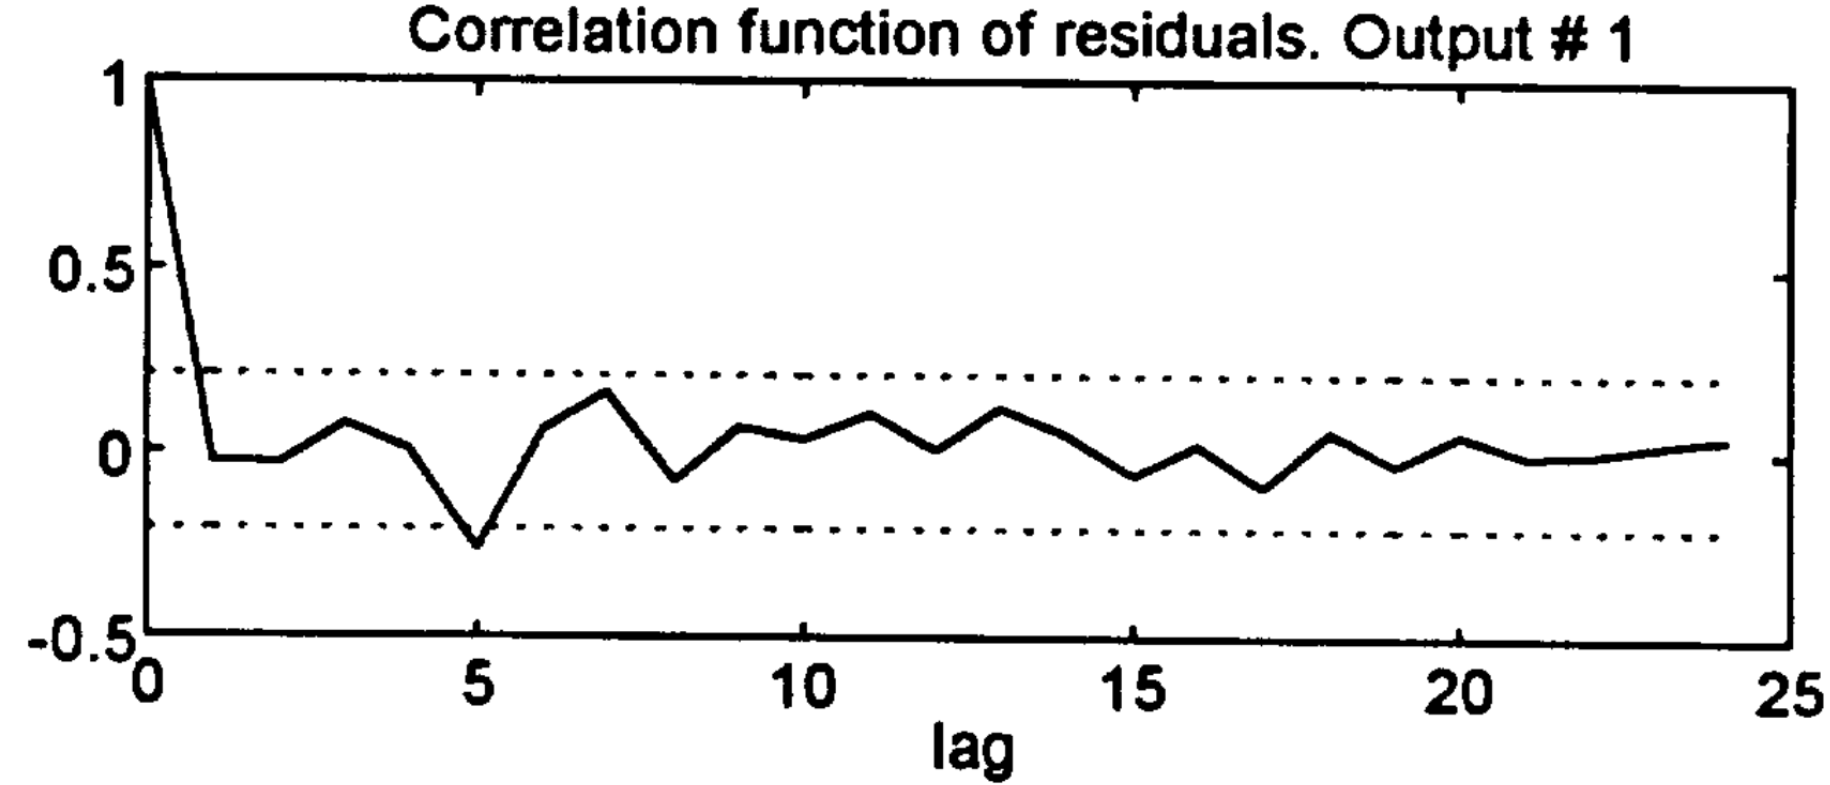
\includegraphics[width=\textwidth]{figures/nasa_xcorr.png}
%     \caption{An autocorrelation plot of a residual signal with which one can validate an identified model. \cite{nasa_white_residual}}
%     \label{fig:nasa_xorr}
% \end{figure}

% \begin{figure}[ht!]
%     \centering
%     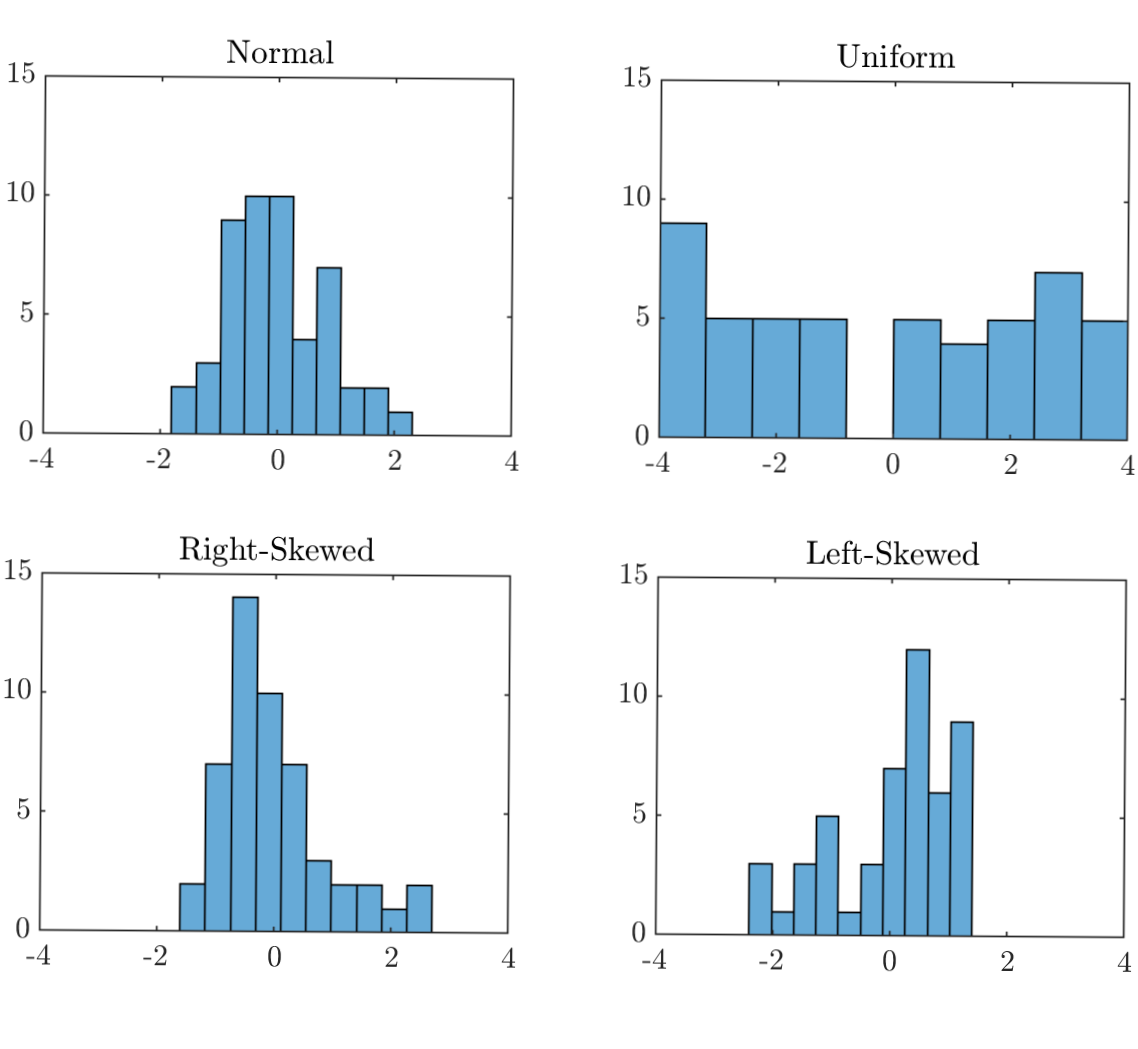
\includegraphics[width=0.8\textwidth]{figures/ex_normplot1.png}
%     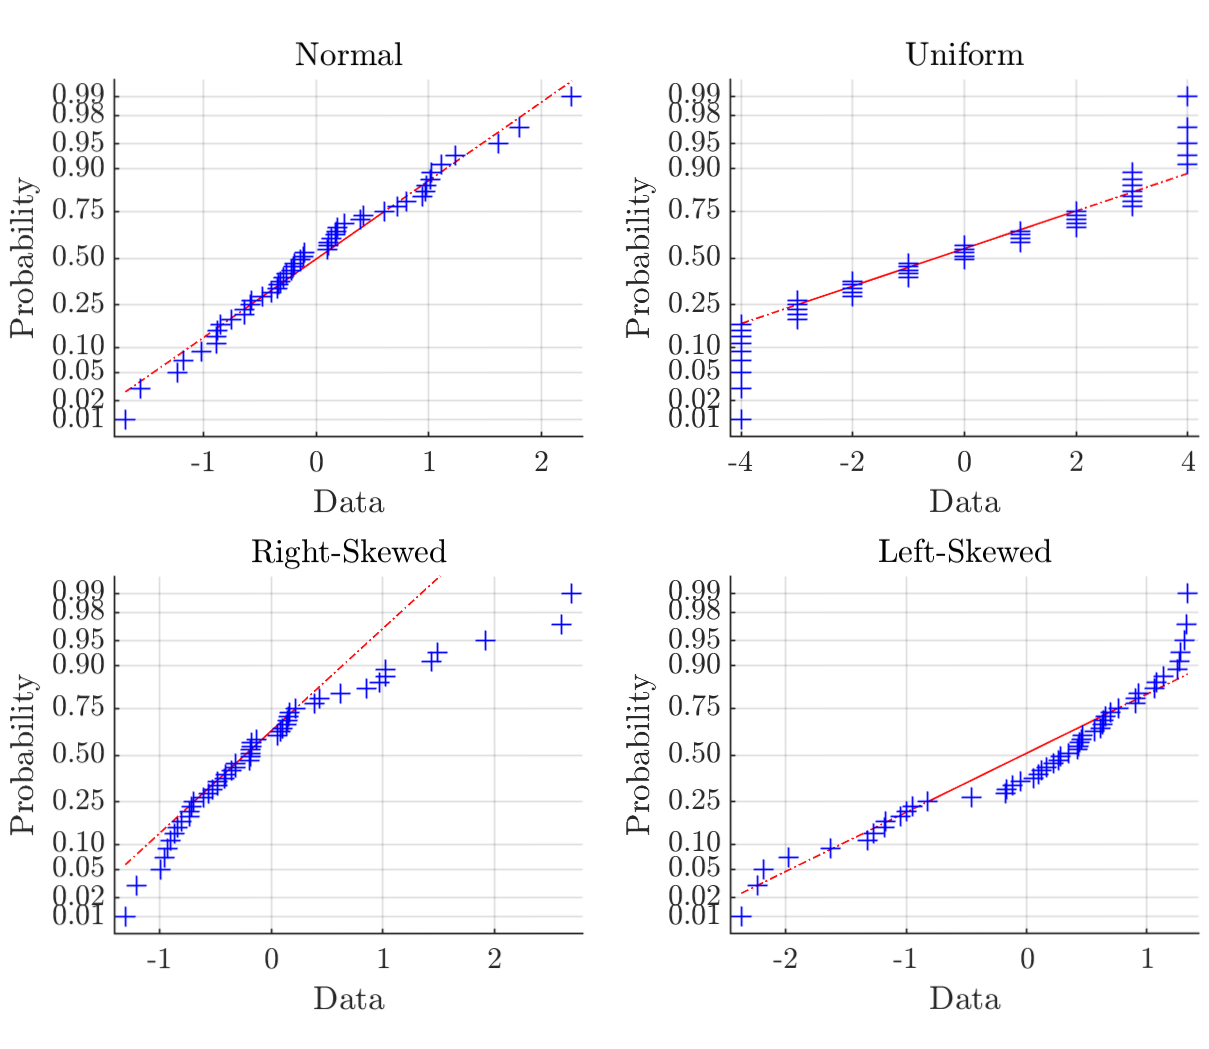
\includegraphics[width=0.8\textwidth]{figures/ex_normplot2.png}
%     \caption{Caption}
%     \label{fig:my_label}
% \end{figure}


The normal probability plot (\texttt{normplot} in MATLAB) is used as a graphical tool to examine the distribution of the residual. % Figures \ref{fig:normplot1} and \ref{fig:normplot2} illustrates the normal probability plots of a few representative distributions. 
By plotting quantiles of the normal distribution (converted into probability values) in a nonlinear scale against the values of each residual datum, one can verify that the residual is normally distributed of the plot appears to be nearly a straight line. Inversely, significant deviations from the straight line indicate skewness or a non-Gaussian distribution. 

All aforementioned characteristics of the obtained residuals are discussed below in full detail.

\begin{figure}[hb]
    \centering
    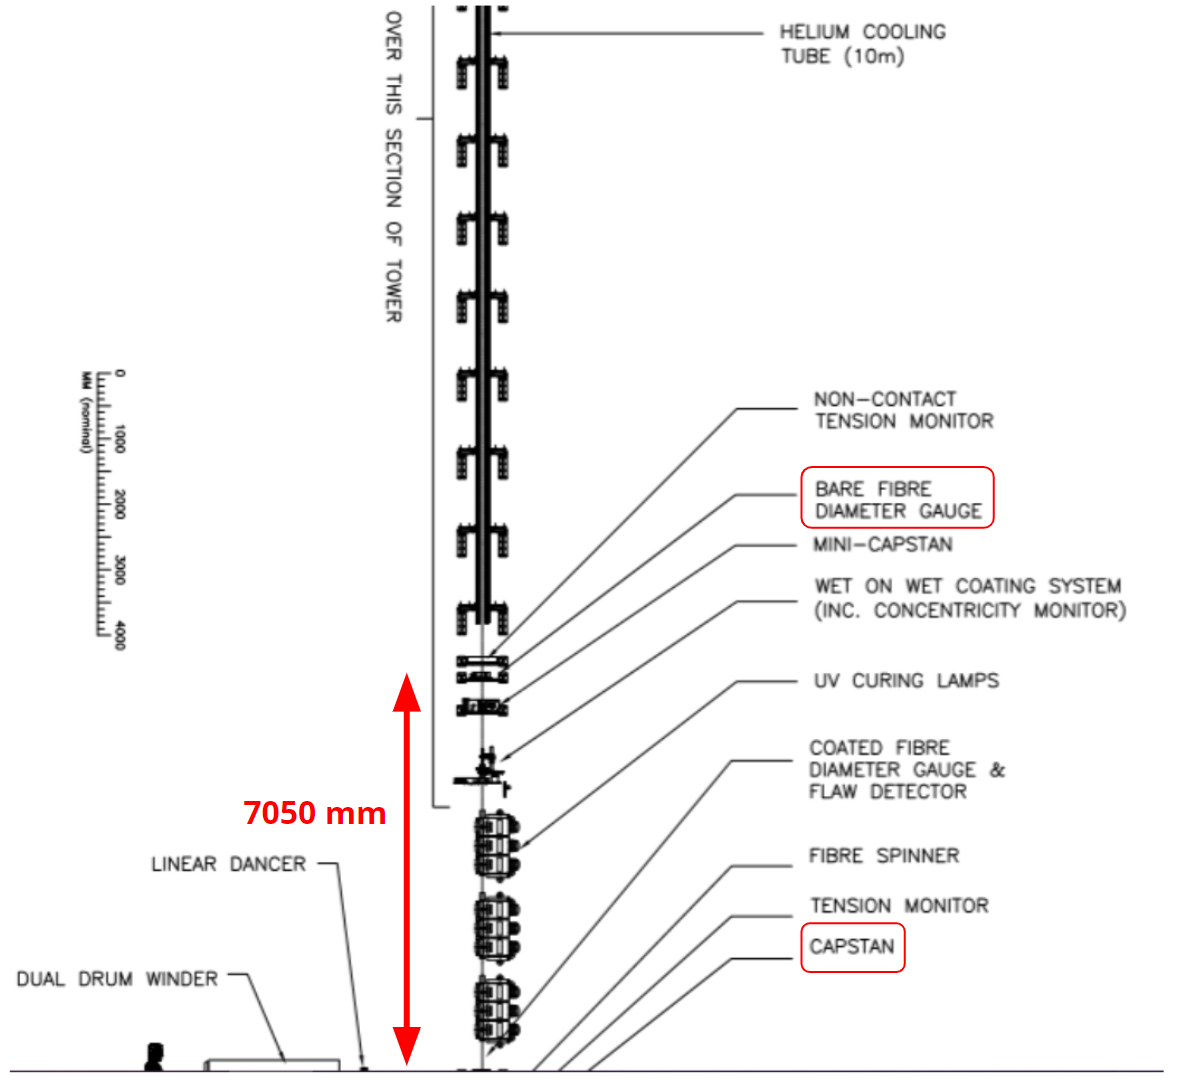
\includegraphics[width=\textwidth]{figures/input_delay.png}
    \caption{A partial mechanical drawing of the fiber drawing structure. (Source: Sterlite Technologies Ltd.)}
    \label{fig:input_delay}
\end{figure}

\section{Case Study: Bare Fiber Diameter Controller} \label{ch:sysid:case}

This section details the modeling of the bare fiber diameter controller within the optical fiber drawing system. The OE and ARMAX model architectures are explored for potential model candidates. All signals referred to below are extracted from files of production data measured on Tower 48. 

\subsection*{A Quick Note on Input Delay}

Both OE and ARMAX models involve modeling the input delay $n_k$ as specified in Equations \ref{eqn:oe} and \ref{eqn:armax}. Due to mechanical constraints in the fiber drawing system, the sensors from which the data were measured are installed in locations far enough that the effect of delay in measurement is of non-negligible significance in modeling. A diagram for a section of the apparatus is shown in Figure \ref{fig:input_delay}. Based on specifications provided by Sterlite, the total distance between the bare fiber diameter gauge (where the real-time BFD is measured) to the capstan pulley (where the capstan speed is measured) is 7050 mm. Given that the sampling time of the logged data is 500 milliseconds and nominal draw speed during operation is around $2500 - 2700$ meters per minute, the input delay (in samples) can be approximated as 
\begin{equation}
    \label{eqn:inp_delay_3}
    500\text{ ms} \times \frac{2700 \text{ m/min}}{7050 \text{ mm}} \approx 3.2 \text{ samples}
\end{equation}
after unit conversion. This provides a reasonable reference point for setting the input delay $n_k$ for the BFD controller when implemented in MATLAB. Thus, for identifying the BFD controller model, the value of $n_k$ is fixed to be $3$ in the grid search process and one layer of the nested \texttt{FOR} loops is eliminated. 

\subsection*{First Look at the Data}

Referring to Figure \ref{fig:stl_system_diag}, the inputs and outputs of the bare fiber diameter (BFD) controller are the measured BFD error and the capstan speed, respectively. Figure \ref{fig:bfd_input_output} illustrates an example of these signals.\footnote{Selected from Week 10, Subbatch 17.} The BFD error signal indicates the deviation of real-time diameter from 125 microns, the nominal BFD value in this manufacturing tower. In each subbatch, the capstan speed is brought from different initial conditions to a desired steady speed of around $2500 - 2700$ meters per minute. 

\begin{figure}[t]
    \centering
    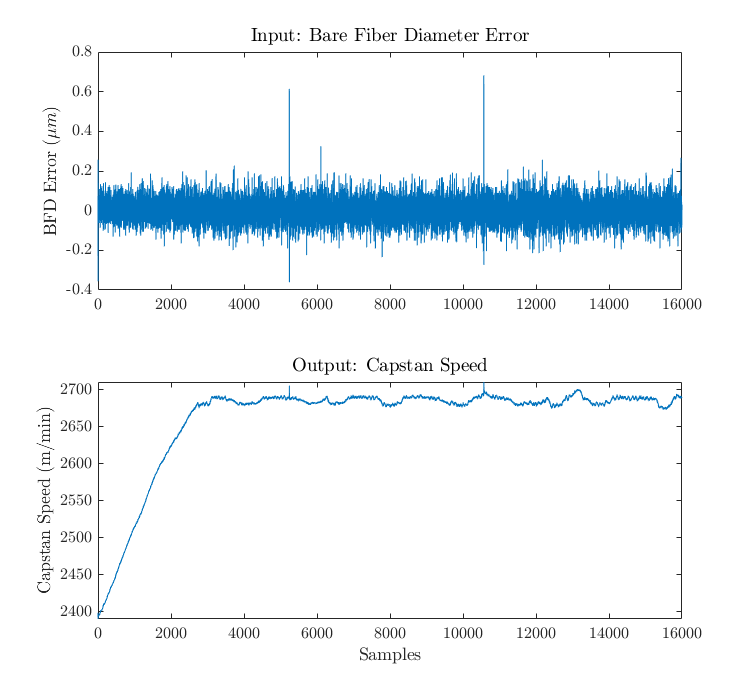
\includegraphics[width=\textwidth]{figures/input_output.png}
    \caption{An example of input and output signals of the bare fiber diameter controller $K_d$.}
    \label{fig:bfd_input_output}
\end{figure}

\subsection*{Comparing Candidate Models}

We first assume the OE structure. After performing the grid search process per Algorithm \ref{alg:grid_search_oe}, subbatches with reasonable fits are tallied and their average accuracy is computed for each column. By sorting the attempted combination of model orders by these metrics, a few best-performing candidate models are identified. Refer to Table \ref{tab:kd_oe}.\footnote{There are 455 subbatches total. A "good" subbatch, as defined in Footnote \ref{ftn:good}, is a subbatch with at least 50\% of percentage accuracy.} Since the identified models performed similarly in average accuracy, Model 1 was selected by the principle of parsimony. 

\begin{table}[h!]
    \centering
    \begin{tabular}{r|cccc}
         & Model 1 & Model 2 & Model 3 & Model 4 \\ \hline
         No. of good subbatches & 358 & 357 & 347 & 345\\
         Average accuracy & 77.30 & 75.98 & 76.27 & 77.14 \\
         Orders & \texttt{[1,4,3]} & \texttt{[1,5,3]} & \texttt{[6,6,3]} & \texttt{[5,5,3]} \\ \hline
    \end{tabular}
    \caption{Results of OE search for bare fiber diameter controller.}
    \label{tab:kd_oe}
\end{table}

The parameters of all the reasonably fitted models for that fixed order, then, were combined to a merged model. In MATLAB's algorithm, it is assumed that the conditions of each experiment are about the same; such an assumption is indeed valid, since the acquired data in each subbatch are measured with the same sensors in the same system. This merging method makes use of the covariance matrices to output the statistically weighted mean as the parameter vector of the merged model, which makes it robust to uncertain measurements in particular experiments (e.g. due to disturbances) \cite{matlab_merge}. This is implemented using the \texttt{merge()} function in MATLAB. Thus we obtain the identified polynomials (a first-order $B(q)$ and a fourth-order $F(q)$ as defined in Equation \ref{eqn:oe}) that characterize the OE model as follows, 
\begin{equation*}
    \begin{split}
        B(q) & = 0.51 q^{-3}\\
        F(q) & = 1 - 0.7012 q^{-1} - 0.0001516 q^{-2} + 0.7 q^{-3} - 0.9986 q^{-4}
    \end{split}
\end{equation*}

\subsection*{Comparison with ARMAX Structure}

The process is similar if we assume the ARMAX structure. The best-performing candidate models returned by the grid search process are tabulated in Table \ref{tab:kd_armax}. 

\begin{table}[h]
    \centering
    \resizebox{\textwidth}{!}{
    \begin{tabular}{r|ccccc}
         & Model 1 & Model 2 & Model 3 & Model 4 & Model 5 \\ \hline
         No. of good subbatches & 248 & 289 & 297 & 297 & 299 \\
         Average accuracy & 66.64 & 63.02 & 60.54 & 59.74 & 59.18 \\
         Orders & \texttt{[4,3,1,3]} & \texttt{[5,5,1,3]} & \texttt{[6,2,1,3]} & \texttt{[7,1,1,3]} & \texttt{[8,1,1,3]} \\ \hline
    \end{tabular}
    }
    \caption{Results of ARMAX search for bare fiber diameter controller.}
    \label{tab:kd_armax}
\end{table}

The first identified model was selected per the principle of parsimony. The ensemble model from merging the data for all subbatches yields the following polynomials, 
\begin{equation*}
    \begin{split}
        A(q) & = 1 - 1.68 q^{-1} + 0.7509 q^{-2} - 0.4594 q^{-3} + 0.3884 q^{-4} \\
        B(q) & = -0.1974 q^{-3} - 0.6482 q^{-4} + 0.8509 q^{-5} \\
        C(q) & = 1 - 0.9813 q^{-1}
    \end{split}
\end{equation*}

Although both OE and ARMAX models have well-conditioned polynomials, the ARMAX model outperforms the OE model in terms of percent fit to validation data, with a $96.68\%$ average and a mean squared error (MSE) of 0.8704. Therefore, the ARMAX model is chosen to be the model of choice for the bare fiber diameter controller; this model will become relevant in the closed-loop simulation later in Section \ref{ch:res:sim}. 

\subsection*{Model Validation} \label{ch:sysid:case:val}

\begin{figure}[p]
    \centering
    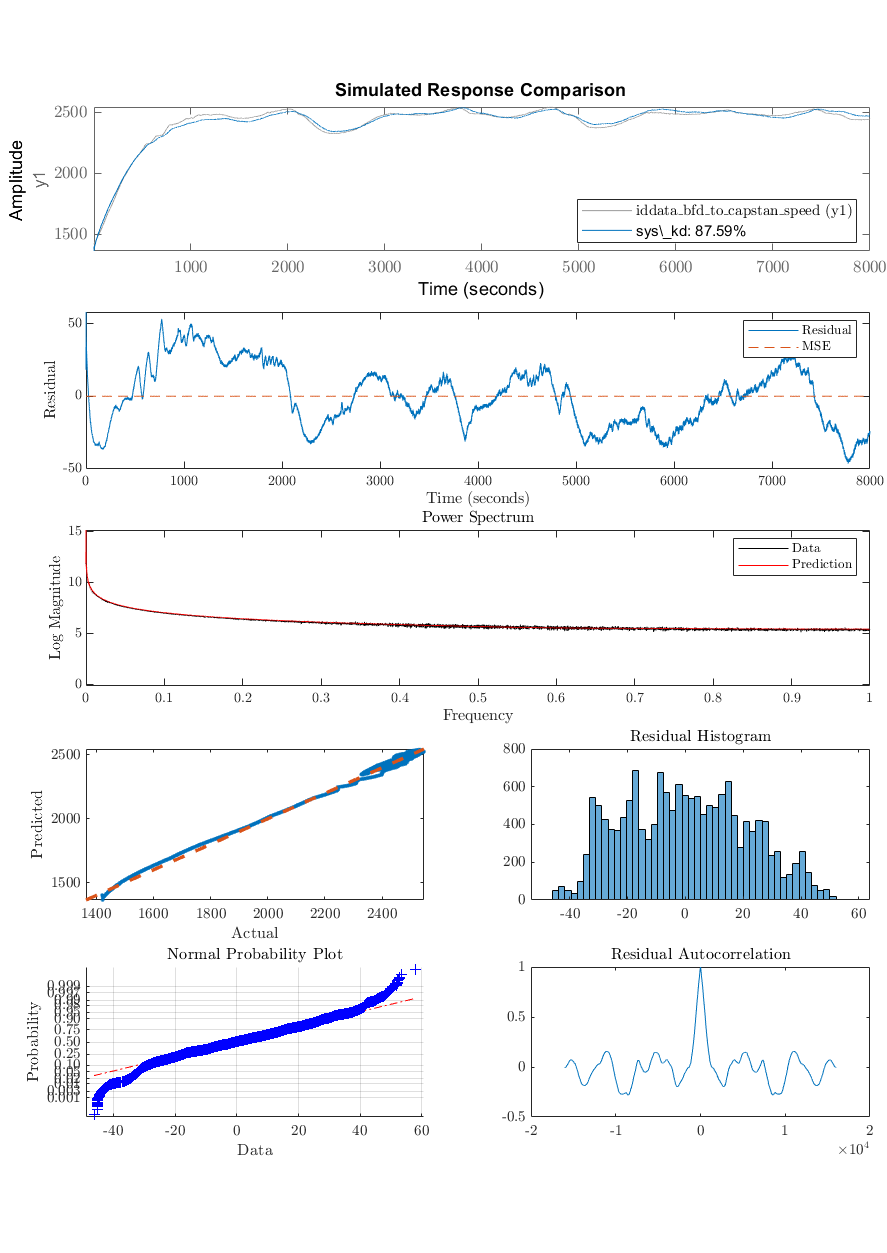
\includegraphics[width=\textwidth]{figures/sysid_validate.png}
    \caption{Time-domain, frequency-domain, and residual analyses performed to validate the ARMAX model for the bare fiber diameter controller.}
    \label{fig:sysid_validate}
\end{figure}

As discussed in Section \ref{ch:sysid:proc:val}, it is necessary to validate the ensemble model by evaluating its performance in terms of time-domain fit percentage, power spectrum, and residual analysis. Figure \ref{fig:sysid_validate} illustrates all such analyses for a typical subbatch of data, while other subbatches behave similarly. The predicted signal by the model has achieved a near-zero MSE and aligns well with the data in the power spectrum, as shown in Figure \ref{fig:sysid_validate}.\footnote{Selected from Week 6, Subbatch 18 in Tower 48 training data.} It then can be said that the model performance are satisfactory in both the time domain and the frequency domain. The autocorrelation of residuals has a peak at zero lag and low magnitude everywhere else; the absence of significant spikes at high order lags indicates that the model is well-specified. Furthermore, as shown in the histogram of residuals and the normal probability plot, the distribution of residuals is not exactly Gaussian nor white noise, which explains the advantage of the ARMAX model due to its ability to parametrize how noise and disturbance enters the system with the $C(q)$ polynomial. 

\begin{figure}[h!]
    \centering
    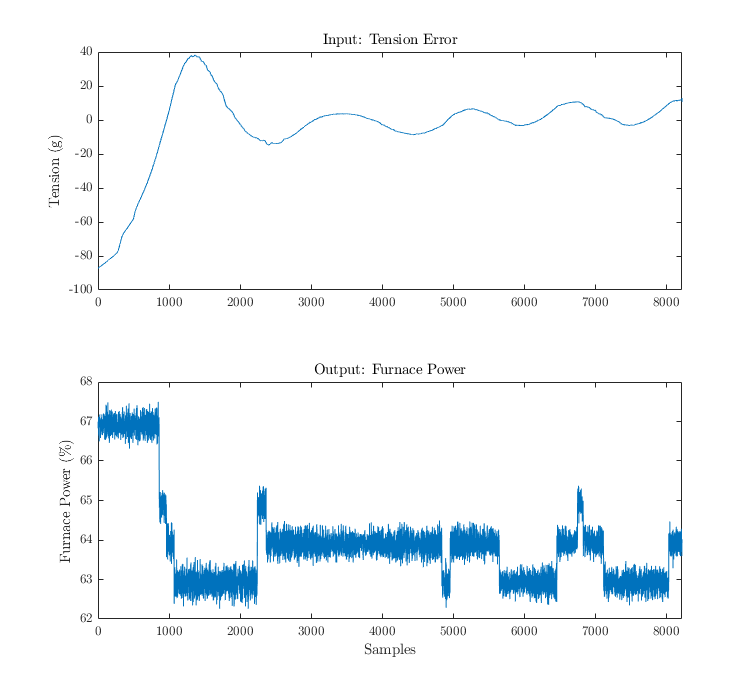
\includegraphics[width=\textwidth]{figures/kt_example2.png}
    \caption{An example of input and output signals of the tension controller $K_t$.}
    \label{fig:kt_example}
\end{figure}

\subsection*{Tension Controller}

The tension controller receives the measured tension error as input and actuates the furnace power as its output (See the system diagram in Figure \ref{fig:stl_system_diag}.) The OE and ARMAX model structures are similarly assumed, and the identification process is identical to that of the bare fiber diameter controller, except that the input delay $n_k$ is no longer fixed and is now part of the search space, i.e. the grid search solves the full general problem posed in Section \ref{ch:sysid:proc:grid}. One of the major differences from the diameter controller discussed above, however, is that the signals measured at the tension controller are much more noisy in nature. Refer to Figure \ref{fig:kt_example} for an illustration.\footnote{Selected from Week 2, Subbatch 7 in Tower 48 training data.} This poses additional challenges in identifying a good fit with high-confidence parameters for this system. The full detail and results of this process is presented in Appendix \ref{apdx:sysid_kt}. 


% The  performances  of  the  developed models were tested using another portion of the data ... 
% Figure  9  is the  error  plot  of  ARX  model  and  Figure  10  is  the ARMAX model. These error plot graphs are the graphs of errors  between  the  actual  output  and  simulated  output.  The  ARX  model  has  achieved  rmse  values  of  0.01869m  while,  ARMAX  model  has  achieved  rmse  values  of  0.00947m. The  model  performance  indices  are  tabulated  in  Table  III.  From  the table, it can be said that ARMAX model has shown betterperformance than ARX model in terms of higher Best Fit and smaller rmse. (https://ieeexplore.ieee.org/stamp/stamp.jsp?tp=&arnumber=8064947)

% address overfitting

% model validation: 
% In addition to the model parametrization and identification, one has to determinethe proper number of parameters for polynomials in (13). Both under- and over-parametrization  have  negative  effects  on  the  results.  Thorough  analysis  ofparametrization  becomes  rather  complicated.  Therefore,  model  validation  wasperformed  by  testing  the  prediction  error  ε(t)  and  by  visually  comparing  themodel and the measured process output. A perfect model generates a white noiseprediction  error  during  minimization. [THAT BOI]

% The criterion, which determines the model is good or not, isthat the accuracy index is over 85%, and the deviations of realparts and imaginary parts of eigenvalues in frequency domainare less than 0.05, compared with the results of MP [1]

% The  use  of  the  MIMO  ARMAX  model  has  many  obviousand potential benefits. The simplest but most important one isthat the model is a measurement-based model, which requiresvery little prior information about the system. Since the MIMOARMAX model selects actual controllable signals in a powersystem  as  the  inputs,  it  is  a  causal  model  which  is  able  tocapture  all  the  dominant  oscillation  modes  and  represent  theentire  power  system  for  oscillation  damping  control. [1]

% Based on the experiment on ARX and ARMAX models for the DC servo motor, we tried to estimate the linear model as  close  as  possible  to  the  real  system.  It  is  done  by  calculating over 100 ARX models and 125 ARMAX models and applying the parsimony principle consisting of choosing the model with fewer parameters and a higher fit. The table below presents the estimated parameters of the proposed  structures  with  the  calculation  of  the  validation  criterions (Best fit and FPE). As  presented  in  table  bellow,  we  can  conclude  that  the  ARMAX model provides a better fit WITH LOWER ORDER (https://ieeexplore.ieee.org/stamp/stamp.jsp?tp=&arnumber=9028015)



\chapter{Results and Discussion} \label{ch:res}

In addition to the presented results in Sections \ref{ch:exp:results} and \ref{ch:sysid:case}, this chapter offers a holistic discussion on the outcome of this study, including the neural-network derived plant dynamics and the system identification of controllers. Section \ref{ch:res:interp} concerns the explainability of identified systems to classical control engineers and general users. Section \ref{ch:res:sim} presents the simulation of closed-loop system in MATLAB using modeled dynamics of each component. Section \ref{ch:res:lim} discusses the limitations of approaches employed by this study and encountered in the field of system identification at large. 

\section{Explainability} \label{ch:res:interp}

As neural network architectures and training data to be modeled become increasingly complex, researchers begin to emphasize the natural explainability of models for general users \cite{explainability1, explainability2}. In this work, the problem of explainability for the process dynamics model and the controller models is addressed through the lens of classical control theory using frequency analysis, specifically through bode plots, a graphical tool to characterize models by their frequency response. 

\subsection{Simulated Bode Plot of a Neural Network Model}

Traditionally, the analytical method of generating a bode plot is via obtaining the transfer function in the Laplace domain from the system's input to the desired output. However, this method loses its feasibility for black-box models including those derived from neural networks. Since developed models from machine learning and system identification approaches are able to make an inference on outputs from arbitrary input signals, simulated bode plots of the process dynamics are generated by making each of the four inputs (namely capstan speed, furnace power, helium temperature, and preform velocity) a sequence of sinusoidal signals of varying frequencies, while maintaining the other signals at their respective average value. For this analysis, the sinusoidal amplitude of each input signal is chosen to be the range of its typical fluctuation in production data, so that the inferred behavior closely resembles that in production. By logarithmically sampling the frequency space up to the Nyquist frequency\footnote{\emph{Nyquist frequency} is defined as half the sampling frequency, which, for the data in this study, is 1 Hz.}, as traditional bode plots do, the system's output signal is plotted in both time- and frequency- domain. Figure \ref{fig:bode_peak} illustrates the system response obtained via inference for one particular frequency; others exhibit similar behaviors. Due to the nonlinearity within the system, the output is not necessarily a single sinusoid; as the frequency-domain plot suggests, a sinusoidal input excites multiple higher frequencies in the system. Among all frequencies, we defined that a frequency is significant if its peak is greater than 5\% of the highest peak. A three-dimensional plot is generated depicting some of these significant frequencies\footnote{\label{ftn:sig}For graphical clarity, only the first 10 significant peaks were plotted for every input frequency.} excited by each input frequency and their respective FFT amplitudes. Refer to Figure \ref{fig:bode_3d}.

\begin{figure}[ht]
    \centering
    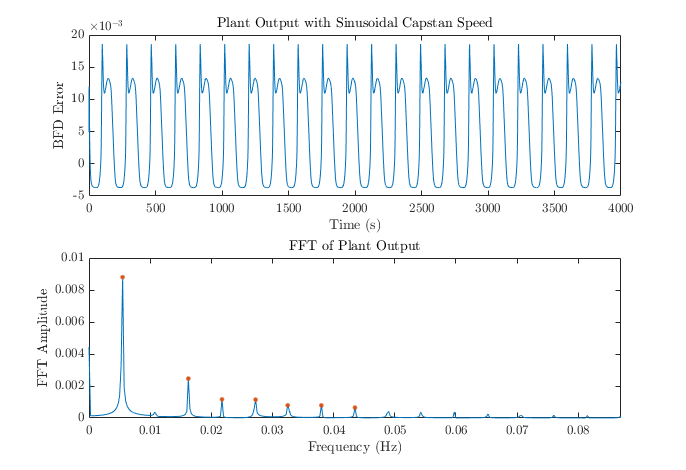
\includegraphics[width=\textwidth]{figures/bode_peak.png}
    \caption{Plant output with a sinusoidal capstan speed of typical amplitude (500 m/min) and frequency of 0.0054 Hz. The red dots mark the significant peaks as defined in Footnote \ref{ftn:sig} on the previous page.}
    \label{fig:bode_peak}
\end{figure}

It is evident that the dominant mode of each sinusoidal response is the one corresponding to the input frequency, shown in Figure \ref{fig:bode_3d} as the diagonal profile. Since the system is nonlinear, it is a common phenomenon that the gain (ratio of output amplitude to input amplitude) is a function dependent on the amplitude of the excitation. We can therefore generate simulated bode plots from each input to the BFD output, with input amplitudes sweeping across their typical ranges. The results of this analysis are shown in Figure \ref{fig:bode_profile}; they correspond to the diagonal profile of Figure \ref{fig:bode_3d} for different excitation amplitudes. It is noteworthy that, for some signals, such as the furnace power and the preform velocity, low-amplitude and high-amplitude inputs display different behaviors. The bifurcations of system behavior in different operational design domains is therefore graphically represented, and it is a smooth transition from one to another. 

\begin{figure}[hp]
    \centering
    \begin{subfigure}[b]{0.49\textwidth}
        \centering
        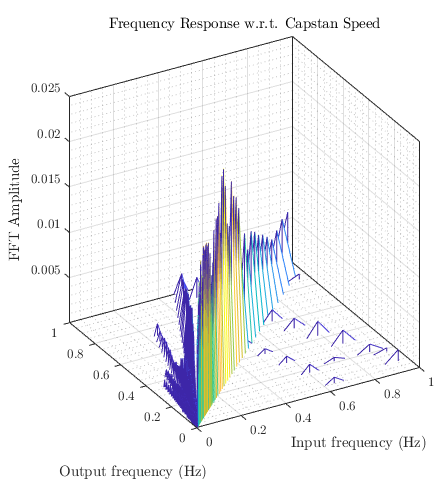
\includegraphics[width=\textwidth]{figures/bode_3d_1.png}
    \end{subfigure}
    \hfill
    \begin{subfigure}[b]{0.49\textwidth}
        \centering
        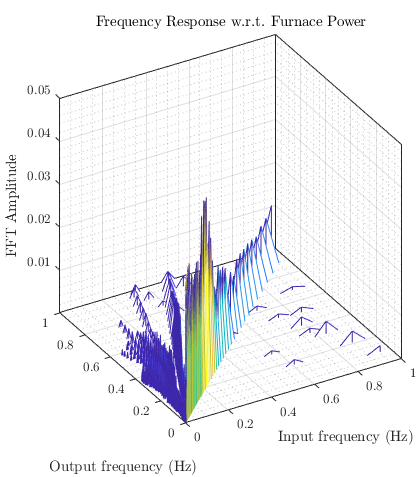
\includegraphics[width=\textwidth]{figures/bode_3d_2.png}
    \end{subfigure}
    
    \begin{subfigure}[b]{0.49\textwidth}
        \centering
        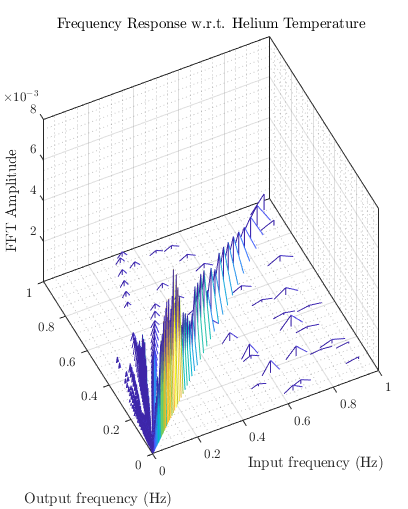
\includegraphics[width=\textwidth]{figures/bode_3d_3.png}
    \end{subfigure}
    \hfill
    \begin{subfigure}[b]{0.49\textwidth}
        \centering
        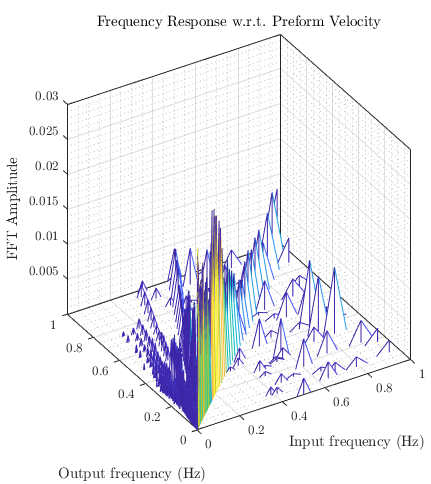
\includegraphics[width=\textwidth]{figures/bode_3d_4.png}
    \end{subfigure}
    
    \caption{3D plots illustrating high frequencies in the neural network plant model excited by sinusoids with a range of input frequencies.}
    \label{fig:bode_3d}
\end{figure}

\begin{figure}[ht]
    \centering
    \begin{subfigure}[b]{0.49\textwidth}
        \centering
        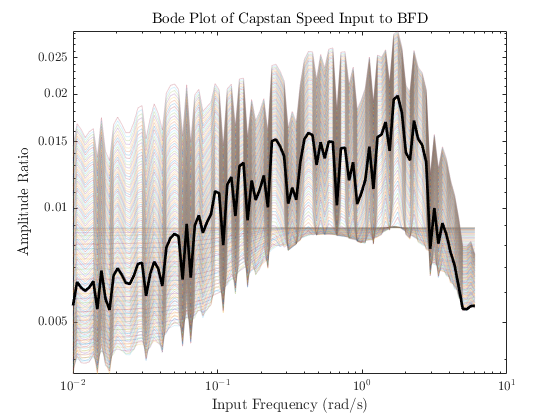
\includegraphics[width=\textwidth]{figures/bode_profile1.png}
    \end{subfigure}
    \hfill
    \begin{subfigure}[b]{0.49\textwidth}
        \centering
        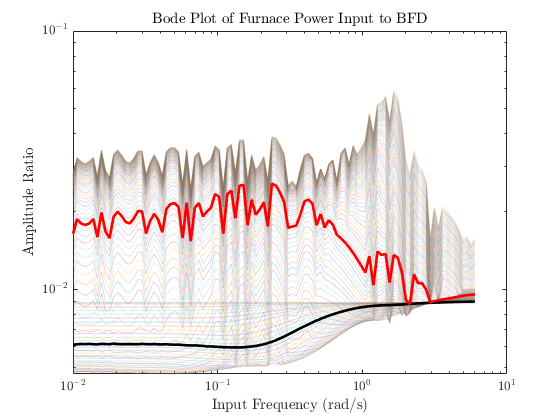
\includegraphics[width=\textwidth]{figures/bode_profile2.png}
    \end{subfigure}
    
    \begin{subfigure}[b]{0.49\textwidth}
        \centering
        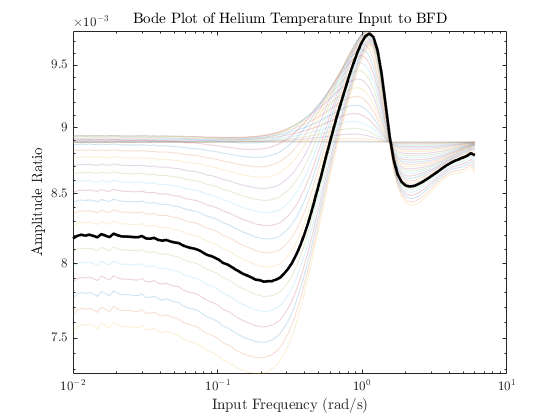
\includegraphics[width=\textwidth]{figures/bode_profile3.png}
    \end{subfigure}
    \hfill
    \begin{subfigure}[b]{0.49\textwidth}
        \centering
        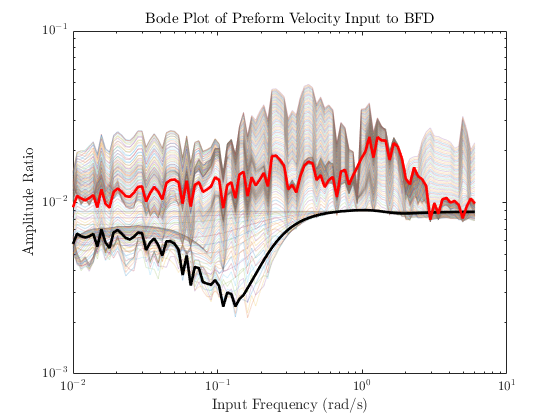
\includegraphics[width=\textwidth]{figures/bode_profile4.png}
    \end{subfigure}
    
    % \caption{Bode plots from each input to the BFD output. Note the variation as a function of excitation amplitudes, a characteristic phenomenon of nonlinear systems.}
    \caption{Bode plots from each input to the BFD output, corresponding to the diagonal profile in Figure \ref{fig:bode_3d}, for different excitation amplitudes. Note the bifurcation of system response for low and high amplitude inputs marked in red and black. }
    \label{fig:bode_profile}
\end{figure}

\subsection{Bode Plot of Subbatch Models to be Merged}

% need to write more ... ensemble model is representative of controller is by ... For instance, for the BFD controller, .... 
% maybe, "similarly for the tension controller, ..."
% change all to plurals

One way to confirm that the ensemble ARMAX model in Section \ref{ch:sysid:case} is representative of the BFD controller's behavior is by investigating the frequency response for each of the subbatch model. Figure \ref{fig:bode_armax_kd_kt} is the overlaid bode plot of the reasonably-fit subbatch models.\footnote{Bode plots depict the good subbatches from Tower 48 data.} All models have approximately equal roll-off rates within the mid- to high- frequency ranges. This consistency among subbatch models is further proven by the well-aligned exponential trend in the phase tending to high frequencies. The exponential drop in phase is attributed to the presence of input delay in the system, equivalently introducing an $e^{-s\Delta T}$ term in the transfer function, a linear factor that appears exponential when graphed logarithmically in the bode plot. ($\Delta T$ denotes the time delay.) This close agreement among the merged subbatch models proved the approach in obtaining the ensemble model reasonable. 

\begin{figure}[hp]
    \centering
    \begin{subfigure}[b]{0.9\textwidth}
        \centering
        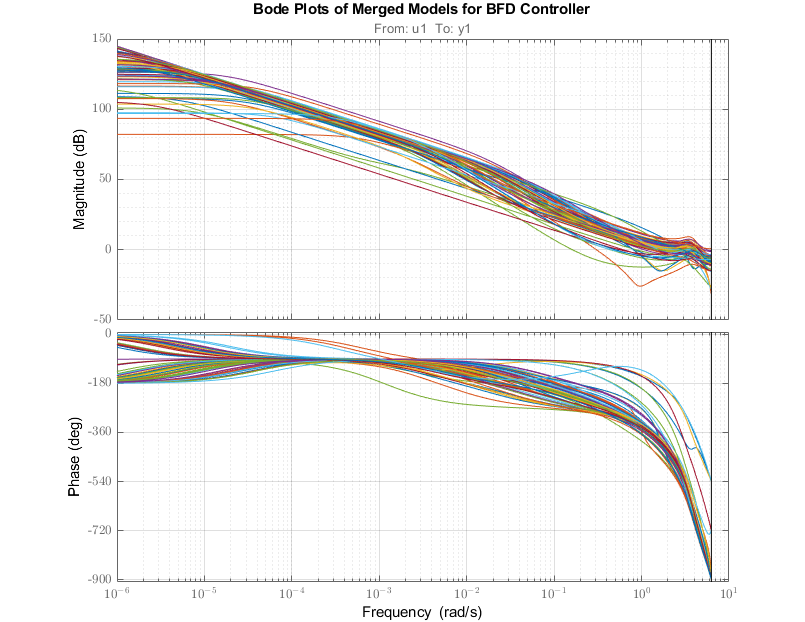
\includegraphics[width=\textwidth]{figures/bode_armax_kd.png}
    \end{subfigure}
    
    \begin{subfigure}[b]{0.9\textwidth}
        \centering
        \includegraphics[width=\textwidth]{figures/bode_armax_kt.png}
    \end{subfigure}
    \caption{Aggregated bode plot of all subbatches to be merged into the ensemble ARMAX model.}
    \label{fig:bode_armax_kd_kt}
\end{figure}

\begin{figure}[ht!]
    \centering
    \includegraphics[width=\textwidth]{figures/closed_loop_simulation.png}
    \caption{Results of the closed-loop simulation on test data. Subplots contain important input and output signals and the predicted BFD by the neural network.}
    \label{fig:closed_loop_sim}
\end{figure}

\section{Closed-Loop Simulation} \label{ch:res:sim}

After developing surrogate models for the as-built process dynamics and controllers, the propagation of signals can be routed according to Figure \ref{fig:stl_system_diag} so that the closed-loop system outputs from identified models can be simulated. With the tension error and BFD error calculated from the feedback signal, the identified model of the BFD controller has an ARMAX structure given by 
\begin{equation}
    \begin{split}
        & y(t) + a_2y(t-1)+a_3y(t-2)+a_4y(t-3)+a_5y(t-4) \\ & = b_4u(t-3)+b_5u(t-4)+b_6u(t-5)+e(t)+c_2e(t-1)
    \end{split}
\end{equation}
Similarly the tension controller has a control law given by 
\begin{equation}
    \begin{split}
        & y(t) + a_2y(t-1)+a_3y(t-2)+a_4y(t-3) \\ & = b_4u(t-3)+b_5u(t-4)+e(t)+c_2e(t-1)+c_3e(t-2)
    \end{split}
\end{equation}
where all $a_i, b_i$ are parameters identified in procedures discussed in Section \ref{ch:sysid:case}. The output $y(t)$ of each signal can be then calculated and used as the input signal to the neural network, which predicts the tension and BFD outputs for the next timestep using the $\texttt{predictAndUpdateState}$ method in MATLAB. With specified BFD and tension setpoints, the closed-loop simulation is now able to simulate the learned controllers' behavior in maintaining these setpoints. The controller outputs then act as inputs to the neural network-derived aggregate plant to simulate the fiber drawing process. Figure \ref{fig:closed_loop_sim} shows this process for one particular subbatch of test data not used for training. This simulation is implemented in a MATLAB script. The source code for this closed-loop simulation and visualization is attached in Appendix \ref{apdx:code:sim}. The hyperlink to the GitHub repository for this study is also provided in the appendix.

\begin{figure}[ht!]
    \centering
    \begin{subfigure}[b]{\textwidth}
        \includegraphics[width=\textwidth]{figures/closed_loop_sim_setpoint.png}
        \caption{Simulation with a change in BFD setpoint. Subfigures illustrate the transient behavior of controllers. }
        \label{fig:sim_setpoint}
    \end{subfigure}
    \begin{subfigure}[b]{0.48\textwidth}
        \centering
        \includegraphics[width=\textwidth]{figures/setpoint_rising.png}
        \caption{Transient behavior on the rising edge of the setpoint change.}
    \end{subfigure}
    \hfill
    \begin{subfigure}[b]{0.48\textwidth}
        \centering
        \includegraphics[width=\textwidth]{figures/setpoint_falling.png}
        \caption{Transient behavior on the falling edge of the setpoint change.}
    \end{subfigure}
\end{figure}

With this simulation as a design tool, a control engineer could visualize the system's transient behavior when there is a change in the setpoint. Figure \ref{fig:sim_setpoint} illustrates a hypothetical experiment in which the BFD setpoint changes from 125 to 135 then back to 125. 

There are profound implications of the controller deployment approach explored in this thesis. This approach builds on the models for the fiber drawing plant and controllers, augmented by first principle equations. With a learned model of the process dynamics and as-built controllers, simulations are built to replicate the system output and verify the accuracy and generalizability of the learned models. In this way, modifications to deployed industrial plants can be done first in simulation, which serves as a digital twin. The predicted output signals become reasonable heuristics to guide the controller improvement process. By defining related components as black-box systems, this study demonstrated that it is possible to identify these systems via machine learning and system identification techniques, integrate them and simulate a full as-built system. Further design improvements to the as-built system could be done first in simulation before implementing them for deployment. In doing so, the simulation serves not only as a digital twin to the hardware in production but also as a design tool for controller development and tuning.

In summary, the recommended procedure is as follows, 

\begin{enumerate}
    \item From data, obtain models for process dynamics, augmented with First Principles models
    \item From data, obtain models for as-built (aggregate) controllers 
    \item Simulate the as-built system with learned process models and as-built controllers
    \item Evaluate the closed-loop simulation, and demonstrate that it can replicate process data and modifications
    \item Use the process model to learn or improve the design of (potentially optimal) controllers 
    \item Simulate the new closed-loop system with improved controllers, evaluate system performance
    \item Deploy improved controllers, collect data, correct if necessary
\end{enumerate}

The approach is applicable to a versatile set of mechanical systems on which an extensive amount of data can be collected. Such examples include coffee roasters, food packaging assemblies, and robotic arms. 

\section{Limitations} \label{ch:res:lim}

The results above and in previous chapters successfully demonstrated the feasibility of this approach to model and simulate mechanical systems in production. Nevertheless, there are several limitations of this work I would like to acknowledge. These limitations stem from theoretical assumptions and inherent imperfections in hardware and in data. Tradeoffs must be made using engineering judgment to mitigate these issues. 

The theory behind autoregressive models like ARMAX assumes that the noise signal that enters the system is uncorrelated to the system's input signal. Many applications in real life cannot guarantee zero correlation. In particular, industrial plants with fast dynamics can have inputs that are more highly correlated with noise, whose frequency range may be similar to that of the process dynamics. Furthermore, parametric methods rely on the local linearization of the plant dynamics. The algorithm built upon linear time-invariant (LTI) systems succumbs to any nonlinearity exhibited by the plant. All the challenges discussed above could potentially lead to biased models for the system dynamics.

The quality of data is a major factor directly correlated with the learning accuracy. Hardware defects are one of the factors attributed to the compromised quality. The heated extrusion process is not perfectly insulated from the ambient environment, and the helium gas flow may have been turbulent in some collected data, which causes disturbance in the extrusion process and adds to the process noise. In addition, most of the data that the neural network was trained on reflected the process dynamics near steady-state, which may lead to an incomplete identified model. It is essential to excite the system with different input signals and initial conditions to obtain more complete data for system behavior. 

% if under control, does not poke the data in different directions, may not excite plants in many ways / modes … may be an incomplete model

Discrete sampling and quantization are additional factors that introduce errors in the data. As mentioned in Section \ref{ch:sysid:case}, the sampling time of the controllers is 100 milliseconds. However, due to the limited computing capacity onboard, the collected data were only logged every 500 milliseconds; the measurements in between were assumed to be zero-order hold. Measurements taken from various components of the plant come from different electrical boxes; the clock synchronization among all the sensors was not verified, either. It is not clear whether there is delay between measurements that were considered to have the same timestamp. Furthermore, sensors also have finite resolution, which is especially evident in the tension controller (e.g. Figure \ref{fig:kt_example}). If the actual value is between two adjacent quantized values, the output signal fluctuates between both values. 

Another shortcoming of sensors is that, as with any measured data from real-world experiments, measurement noise from sensors must be taken into account in data analysis. Visualizations in Chapter \ref{ch:sysid} already demonstrated that measured data are often corrupted by noise. (See Figures \ref{fig:bfd_input_output} and \ref{fig:kt_example}.) If the noise dynamics were modeled adequately, the system identification technique can better recover the underlying process dynamics from a noisy signal. However, the noise specifications of sensors on the plant happen to span a similar frequency range than high-frequency dynamics of the BFD, which we were interested in exploring. This added difficulty in achieving high accuracies using the system identification approaches. Noise also makes finite difference elements of the control loop highly susceptible to instability. % REFER TO LOOK UP TABLE 
The use of finite difference is also implicit in converting real systems to the general time-series model (refer to Equation \ref{eqn:pid_fd}). As claimed by Trischler et al., chaos can occur in one-dimensional finite-difference systems, in contrast to continuous differential equations where three dimensions are required \cite{trischler}.

% quality of data (coming from hardware defects - not insulated with ambient, sampling & quantization errors, clock not sync'ed, noisy sensors -> finite difference bad, chaos can occur in one-dimensional finite-difference systems, while three dimensions are required for chaos in continuous systems)
% noisy sensors - frequency specs overlaps with high freq dynamics, makes recovering original dynamics using sys id more difficult

There remain a few open challenges in developing purely data-based models for controllers. 

\begin{enumerate}
    \item Black-box models are data-hungry and data-specific. As mentioned above, the accuracy of a model depends on the hardware involved and the quality of measurement data. A low volume of data would also result in a high variance of the estimated parameters. %, the effect of which has been illustrated in Figure \ref{}. % CITE MODALITY PLOT
    An adequate model of a system should demonstrate good generalization capabilities on validation data. The combination of volume and specificity of the required data makes black-box system identification a challenging problem. 

    \item Striking a balance between performance and robustness is difficult. This has been the age-old question across the system identification, control, and machine learning communities, although referred to by different terms. An overly trained machine learning model is subject to \emph{overfitting}, which means its predictive performance degrades outside of training dataset it has seen. In system identification, a model of higher order may fit the input-output data to better accuracy, but it is difficult to justify with first principles and may face a similar problem with an overfitted model. Parameters within a controller must also be tuned to balance higher peak performance in specific scenario(s) vs. a more robust performance over a wider set of operational design domains \cite{tan_et_al}.
    % high order that fits well or low order ... ? % control - good in some ODD bad in others, machine learning - overfitting, RL -  trade-off. % QUOTE THE PAPER FROM THE TALK THE OTHER DAY (2022-03, SIM-TO-REAL LEARNING AGILE LOCOMOTION FOR QUADRUPED ROBOTS, TAN ET AL, 2018)
    
    \item From a classical controls perspective, controllers and systems identified by data-driven approaches (i.e. via neural networks and system identification techniques) may involve complex poles and zeros when analyzed in the Laplace domain. % CITE SOMETHING?
    It is also not straightforward as to how to further fine-tune them to optimize for custom specifications or specific frequency-related properties. 
    
    \item In many machine learning applications, the technique of \emph{transfer learning} has shown great promise \cite{transfer_learning_sdc, transfer_learning_cnn}. Weights and architectures from pre-trained models used almost directly, with some modifications, to solve similar problems. However, for controllers (especially in an established plant in production), the specificity of the plant and the lack of literature both may pose challenges in applying the transfer learning technique. 
\end{enumerate}

In fact, these open questions are not unique to this project. A large amount of literature (some cited above) also assessed each of these limitations in different applications. Section \ref{ch:concl:future_work} also details ways that some of these can be addressed in the future of this ongoing project. 
\chapter{Conclusion}

\section{Contributions}

The principle contributions of this thesis are manifold. Firstly, the methodology developed in this thesis is beneficial to Sterlite and the manufacturing community at large. The developed closed-loop simulation could replace the traditional, iterative way of controller bringup; industrial facilities can make use of a digital twin as a design tool to optimize controllers in production. The procedure employed in this thesis, mentioned in Section \ref{ch:intro:motiv}, serves as a guideline to data-driven deployment. Furthermore, this thesis addressed a number of problems across the machine learning and control communities. Statistical models were proven to be immensely beneficial in developing a high-confidence model, from collected data of limited quality in the presence of noise and disturbances. Said approach is widely applicable in the areas of data analytics, robotics, controls, and beyond. 

\section{Conclusion}

This thesis demonstrated the feasibility of surrogate modeling for an optical fiber extrusion system, black-box system identification of its controllers, and developing a closed-loop simulation for the plant in production. The fiber drawing plant was modeled using a trained LSTM neural network, and the performance of which was evaluated both in time-domain using RMSE and in frequency-domain using power spectrum. Black-box systems for the controllers modulating input signals to the plant were developed. With the orders of the characteristic polynomials selected and the system parameters identified, an ensemble model of all subbatches within the fixed order was generated and validated. All developed models demonstrated that they are able to integrate into a closed-loop simulation to replicate real system behavior, achieving their purpose as a digital twin and a design tool for controllers in production. 


\section{Future Work} \label{ch:concl:future_work}

There are several areas of this work that warrant future research, elaborated in the subsections below. 

\subsubsection{Neural Network}

As discussed in Section \ref{ch:exp:data}, the current pre-processing pipeline restricts the training data by the upper and lower thresholds of the BFD. This approach places more emphasis on the steady-state region of the production data; as a consequence, the trained model learns and predicts the steady-state process dynamics with higher accuracy. Future iterations of this work could make use of the recorded flag in our data indicating whether the PID controller is engaged. By training on the data whenever the controller \emph{is} engaged, the learned model could observe more of the (potentially nonlinear) dynamics in which the BFD starts with different initial conditions and is brought to steady-state. Learning this insight could make the model more robust to disturbances in simulated dynamics. 

The fundamental assumption of the neural network approach to black-box system modeling is that a neural network is complex enough to adequately model the underlying physics. However, having physical insight into the system's governing equation would be immensely helpful. Another approach commonly employed in literature is to use neural networks to model the residual dynamics not captured by the fundamental structure \cite{tossingbot_zeng_residual_physics}. One of the challenges I foresee, though, is obtaining a sufficiently elaborate physical model for the complex process dynamics in fiber extrusion. It is crucial that the analytical equations are able to adequately model most of the dynamics, so that the neural network is used for fine-tuning purposes only. There must be engineering judgment involved in regularizing the data-driven residual term, so to prevent it from dominating the terms in the rest of the equation. 

\subsubsection{System Identification}

Following the procedures outlined in \ref{ch:sysid:proc}, future research efforts could explore other data-based models. MATLAB's System Identification Toolbox also provides machinery to identify the Box-Jenkins (BJ) model, the NonLinear AutoRegressive model with eXogeneous input (NLARX), and many more. It may be worthwhile to experiment with each of their respective orders and compare the performance with existing results. 

There are two prevalent metrics for system identification methodologies. The comparisons shown in Section \ref{ch:sysid:case} used the \emph{output error criterion}, in which system parameters are optimized for the lowest error in the final output, namely the NRMSE as defined in Equation \eqref{eqn:sysid_fit}. The other approach is to use the \emph{equation error criterion}, which resets the model to the data at every timestep and tunes the system parameters to minimize the one-step prediction errors over all timesteps of the simulation horizon \cite{equation_output_error, ljung1999system}. Since the equation error could be obtained via least squares regression, which is quadratic in the parameters, this convex parametrization is easier to compute and more accurate, but the identified system may be unstable due to accumulated errors over time. The output error criterion is a more robust methodology, but the nonconvex optimization involved in the computation makes it less favorable \cite{tedrake_manipulation_lec_error}. It would yield interesting results if a comparison study is conducted, or if a hybrid method is used, e.g. obtain an initial estimate of system parameters with the equation error approach, then fine-tune them with nonlinear optimization in the output error. 

Despite the challenges addressed, I remain optimistic for the future of this ongoing research endeavor. 

\appendix
\chapter{System Identification Results for Tension Controller} \label{apdx:sysid_kt}

Following the approach described in \ref{ch:sysid:case}, we first assume the OE structure. The grid search process over orders $[n_a, n_b, n_k]$ subject to constraints in \eqref{eqn:oe_bounds} returns the highest performing candidate models as follows,

\begin{table}[h]
    \centering
    \begin{tabular}{r|cccc}
         & Model 1 & Model 2 & Model 3 & Model 4 \\ \hline
         No. of good subbatches & 249 & 259 & 255 & 259 \\
         Average accuracy & 55.62 & 54.38 & 52.75 & 51.89 \\
         Orders & \texttt{[9,10,4]} & \texttt{[10,10,3]} & \texttt{[4,5,4]} & \texttt{[6,7,4]} \\ \hline
    \end{tabular}
    \caption{Results of OE search for tension controller.}
    \label{tab:kt_oe}
\end{table}

As previously addressed in Section \ref{ch:sysid:proc:order}, a high order fit would lose its reliability and robustness, despite its marginally better performance. Therefore Model 3 was selected to generate the ensemble model, which has the following characteristic polynomials, 
\begin{equation*}
    \begin{split}
        B(q) & = 0.02128 q^{-4} - 0.04466 q^{-5} + 0.06583 q^{-6} - 0.04242 q^{-7} \\            
        F(q) & = 1 - 0.4937 q^{-1} - 0.1593 q^{-2} - 0.8731 q^{-3} + 0.2688 q^{-4} + 0.2573 q^{-5}
    \end{split}
\end{equation*}

Similarly, assuming the ARMAX structure, the grid search returns the following candidate models, 
\begin{table}[ht]
    \centering
    \begin{tabular}{r|cccc}
         & Model 1 & Model 2 & Model 3 & Model 4 \\ \hline
         No. of good subbatches & 216 & 215 & 212 & 209 \\
         Average accuracy & 49.24 & 51.27 & 50.20 & 50.28 \\
         Validation average fit & 72.15 & 71.73 & 71.44 & 72.24 \\
         Orders & \texttt{[4,3,3,4]} & \texttt{[4,4,3,4]} & \texttt{[3,4,4,4]} & \texttt{[3,2,2,3]} \\ \hline
    \end{tabular}
    \caption{Results of ARMAX search for tension controller.}
    \label{tab:kt_armax}
\end{table}

Inspecting all candidate models, Model 4 was selected since it slightly outperforms Model 1 in the average fit percent to validation data; Thus, it is also the model of choice used in the closed-loop simulation. The characteristic polynomials are identified as follows, 
\begin{equation*}
    \begin{split}
        A(q) & = 1 - 0.6357 q^{-1} - 0.3797 q^{-2} + 0.01532 q^{-3}\\
        B(q) & = 3.299\times 10^{-4} q^{-3} - 2.847\times 10^{-4} q^{-4}\\
        C(q) & = 1 - 0.3122 q^{-1} - 0.2831 q^{-2}\\
    \end{split}
\end{equation*}

The selected model is similarly validated; Figure \ref{fig:sysid_validate_kt} illustrates the time-domain, frequency-domain, and residual analyses involved. Although the signals are corrupted by noise, the model performance are satisfactory in all metrics indicated per Section \ref{ch:sysid:case:val}.

\begin{figure}
    \centering
    \includegraphics[width=\textwidth]{figures/sysid_validate_kt.png}
    \caption{Time-domain, frequency-domain, and residual analyses performed to validate the ARMAX model for the tension controller.}
    \label{fig:sysid_validate_kt}
\end{figure}

% This is an example of how you would use tgrind to include an example
% of source code; it is commented out in this template since the code
% example file does not exist. To use it, you need to remove the '%' on the
% beginning of the line, and insert your own information in the call.
%
%\tagrind[htbp]{code/pmn.s.tex}{Code sample}{opt:pmn}


\chapter{MATLAB Source Code Excerpt} \label{apdx:code}

All code for this thesis work is written in MATLAB and is version controlled in GitHub. Please refer to \href{https://github.com/gcfc/fiber-draw}{\underline{this GitHub repository}} (\href{https://github.com/gcfc/fiber-draw}{https://github.com/gcfc/fiber-draw}) for the complete source code. 

Below are some meaningful excerpts demonstrating various key components mentioned throughout the thesis. 

\section{Architecture Exploration for Plant Dynamics}

Filename: $\texttt{architecture\_experiment.m}$
\begin{lstlisting}
load('alldatatrain\all_data_processed_4in_1out_yremove125.mat', 'Xdata', 'Ydata', 'x_train', 'y_train', 'x_test', 'y_test', 'filenames')   

simple_lstm = create_simple_lstm(x_train, y_train);
[simple_lstm, simple_lstm_info] = train_lstm(simple_lstm, x_train, y_train, x_test, y_test, 64);

deep_lstm = create_deep_lstm(x_train, y_train);
[deep_lstm, deep_lstm_info] = train_lstm(deep_lstm, x_train, y_train, x_test, y_test, 16);

simple_bilstm = create_simple_bilstm(x_train, y_train);
[simple_bilstm, simple_bilstm_info] = train_lstm(simple_bilstm, x_train, y_train, x_test, y_test, 16);

side_by_side_3_lstm = create_3_side_by_side_lstm(x_train, y_train);
[side_by_side_3_lstm, side_by_side_3_lstm_info] = train_lstm(side_by_side_3_lstm, x_train, y_train, x_test, y_test, 32);

save('results/architecture_experiment.mat', 'simple_lstm', 'simple_lstm_info', 'deep_lstm', 'deep_lstm_info', 'simple_bilstm', 'simple_bilstm_info', 'side_by_side_3_lstm', 'side_by_side_3_lstm_info');
\end{lstlisting}

Function: $\texttt{train\_lstm.m}$
\begin{lstlisting}

function [net, info] = train_lstm(net, x_train, y_train, x_test, y_test, miniBatchSize)

maxEpochs = 250;

options = trainingOptions('adam', ...
            'InitialLearnRate',         0.01, ...
            'OutputNetwork',            'best-validation-loss', ...
            'MaxEpochs',                maxEpochs, ...
            'MiniBatchSize',            miniBatchSize, ...
            'GradientThreshold',        10, ...
            'SequenceLength',           'longest', ...  % padding
            'SequencePaddingDirection', 'right', ...   
            'SequencePaddingValue',     0, ...               
            'Shuffle',                  'once', ...
            'Plots',                    'training-progress',...
            'LearnRateSchedule',        'piecewise',...
            'LearnRateDropPeriod',      100,... 
            'Verbose',                  1, ...
            'ValidationData',           {x_test, y_test});
[net, info] = trainNetwork(x_train,y_train,net,options);
end
\end{lstlisting}

Function: $\texttt{create\_simple\_lstm.m}$
\begin{lstlisting}
function [Networklayers] = create_simple_lstm(xTrain, yTrain)

[featureDimension,~ = size(xTrain{1});
[numResponses, ~]   = size(yTrain{1});

Networklayers = [sequenceInputLayer(featureDimension, 'Normalization','zscore') ...
    lstmLayer(128) ...
    fullyConnectedLayer(numResponses) ...
    regressionLayer];
end
\end{lstlisting}

Function: $\texttt{create\_simple\_bilstm.m}$
\begin{lstlisting}
function [Networklayers] = create_simple_bilstm(xTrain, yTrain)

[featureDimension, ~] = size(xTrain{1});
[numResponses, ~]     = size(yTrain{1});

Networklayers = [sequenceInputLayer(featureDimension, 'Normalization','zscore') ...
    bilstmLayer(128) ...
    fullyConnectedLayer(numResponses) ...
    regressionLayer];
end
\end{lstlisting}

Function: $\texttt{create\_3\_side\_by\_side\_lstm.m}$
\begin{lstlisting}
function [Networklayers] = create_3_side_by_side_lstm(xTrain, yTrain)

[featureDimension, ~] = size(xTrain{1});
[numResponses, ~]     = size(yTrain{1});

lgraph = layerGraph();

tempLayers = sequenceInputLayer(featureDimension,'Name','sequence');
lgraph = addLayers(lgraph,tempLayers);

tempLayers = lstmLayer(128,'Name','lstm_2');
lgraph = addLayers(lgraph,tempLayers);

tempLayers = lstmLayer(128,'Name','lstm_1');
lgraph = addLayers(lgraph,tempLayers);

tempLayers = lstmLayer(128,'Name','lstm_3');
lgraph = addLayers(lgraph,tempLayers);

tempLayers = [
    concatenationLayer(1,3,'Name','concat')
    fullyConnectedLayer(numResponses,'Name','fc')
    regressionLayer('Name','regressionoutput')];
lgraph = addLayers(lgraph,tempLayers);

% clean up helper variable
clear tempLayers;

lgraph = connectLayers(lgraph,'sequence','lstm_2');
lgraph = connectLayers(lgraph,'sequence','lstm_1');
lgraph = connectLayers(lgraph,'sequence','lstm_3');
lgraph = connectLayers(lgraph,'lstm_2','concat/in2');
lgraph = connectLayers(lgraph,'lstm_1','concat/in1');
lgraph = connectLayers(lgraph,'lstm_3','concat/in3');

Networklayers = lgraph;
\end{lstlisting}

Function: $\texttt{create\_deep\_lstm.m}$
\begin{lstlisting}
function [Networklayers] = create_deep_lstm(xTrain, yTrain)

[featureDimension, ~] = size(xTrain{1});
[numResponses, ~]     = size(yTrain{1});

Networklayers = [sequenceInputLayer(featureDimension, 'Normalization','zscore') ...
    lstmLayer(128) ...
    lstmLayer(128) ...
    lstmLayer(128) ...
    fullyConnectedLayer(numResponses) ...
    regressionLayer];
end
\end{lstlisting}

\section{Long-Term Drift in RMSE}

Filename: $\texttt{week\_drift\_subbatch\_analysis.m}$
\begin{lstlisting}
load('run_results\architecture_experiment.mat')
load('alldatatrain\all_data_processed_4in_1out_yremove125.mat')

net = deep_lstm.resetState();

combined_Xdata = cat(2, Xdata{:});
combined_Ydata = cat(2, Ydata{:});
y_pred = net.predict(combined_Xdata, 'MiniBatchSize', 1);

errors = zeros(1,length(y_pred));
for b = 1:length(y_pred)
    errors(b) = sqrt(sum((y_pred{b} - combined_Ydata{b}).^2/length(y_pred{b})));
end

figure; plot(errors); title('Model RMSE over Time'); 
ylabel('RMSE'); xlabel('Subbatch'); xlim([0 length(errors)])
latexify_plot;
\end{lstlisting}

\section{Grid Search and Model Selection}

Filename: $\texttt{sys\_id\_pipeline.m}$
\begin{lstlisting}
%% Main
clear; clc; close all;

[num_good_subbatches, average_accuracy] = grid_search_oe('kd', 10, false); 
writematrix([num_good_subbatches; average_accuracy], 'kd_oe_results.xlsx');

[num_good_subbatches, average_accuracy] = grid_search_oe('kt', 10, false);
writematrix([num_good_subbatches; average_accuracy], 'kt_oe_results.xlsx');

[num_good_subbatches, average_accuracy] = grid_search_armax('kd', 8, false); 
writematrix([num_good_subbatches; average_accuracy], 'kd_armax_results.xlsx');

[num_good_subbatches, average_accuracy] = grid_search_armax('kt', 8, false);
writematrix([num_good_subbatches; average_accuracy], 'kt_armax_results.xlsx');

[all_sys, all_iddata] = merge_models('kd', 'oe', [1 4 3], false);
[all_sys, all_iddata] = merge_models('kd', 'armax', [4 3 1 3], false);
[all_sys, all_iddata] = merge_models('kt', 'oe', [4 5 4], false);
[all_sys, all_iddata] = merge_models('kt', 'armax', [3 2 2 3], false);

%% Function Definitions
function [all_file_data, dt] = load_data()
    % parameters
    strDataPath = 'C:\fakepath\MIT_DrawData_48and51\';
    all_files   = dir(strDataPath);
    curr_path   = 'C:\fakepath\Desktop\fiber-draw';
    
    % BatchInfo Parameters
    bXLSLoad = 1;
    bPlotAll = 0;
    bPlot_each_preform_on_subplot = 1;
    bPlot_each_preform_on_subplot_with_inrangesubbatches_ = 1;
    loBFD = 124;
    hiBFD = 126;
    nTower = 48; % The tower number
    subbatchMinLen 	= 2000; 
    subbatchMaxLen  = 16000;
    x_columns = ['cpspdactval', 'frnpwrmv', 'pfspdactval'];
    y_columns = ['barefibrediadisplay', 'tenncmv'];
    
    % Subbatch Parameters
    fltLEN = 21;
    bPlot = 0; 
    PrefltLEN = 1;
    dt = 0.5;
    
    if exist('all_file_data.mat', 'file') ~= 2
        all_file_data = cell(length(all_files),2);
    
        for i = 1:length(all_files)
            curr_file = all_files(i);
            if ~curr_file.isdir
                % get batch info
                [BatchInfo, STRDEF] = stl_load_batchinfo(bXLSLoad, strDataPath, curr_file.name, nTower, bPlotAll, bPlot_each_preform_on_subplot_with_inrangesubbatches_, bPlot_each_preform_on_subplot, loBFD, hiBFD, subbatchMinLen, subbatchMaxLen, x_columns, y_columns);
    
                % turn it into a train / test array
                [XTrainTranspose, YTrainTranspose] = stl_prep_training_data(BatchInfo, STRDEF, x_columns, y_columns, fltLEN, PrefltLEN, bPlot, 0, 0);
    
                all_file_data{i,1} = XTrainTranspose;
                all_file_data{i,2} = YTrainTranspose;
            end
            fprintf('%d/%d files loaded...\n', i, length(all_files))
        end
    
        save('all_file_data','all_file_data')
    else
        load('all_file_data.mat', 'all_file_data');
    end
    
    disp('Done Loading!')
end

function [num_good_subbatches, average_accuracy] = grid_search_oe(controller, max_order, plot_sysid_process)

    [all_file_data, dt] = load_data();
    
    switch controller
        case 'kd'
            all_nk = [3];
        case 'kt'
            all_nk = 1:4;
        otherwise
            error("invalid controller argument!")
    end
    
    fit_matrix = cell(length(all_file_data), 1);
    folder_name = sprintf("oe_%s_plots", controller);
    
    if plot_sysid_process && exist(folder_name, 'dir') ~= 7
        mkdir(folder_name);
    end
    
    for file_ind = 1:16 % tower 48
        curr_file = all_file_data{file_ind,1};
        if ~isempty(curr_file)
    
            % load from loaded data
            XTrainTranspose = all_file_data{file_ind,1};
            YTrainTranspose = all_file_data{file_ind,2};
    
            fit_matrix{file_ind} = zeros(length(XTrainTranspose), max_order^2*length(all_nk));
    
            for i = 1:length(XTrainTranspose)
                xs = cell2mat(XTrainTranspose(i));
                ys = cell2mat(YTrainTranspose(i));
                capstan_speed = xs(1,:); furnace_power = xs(2,:); preform_speed = xs(3,:);
                bfd = ys(1,:); tension = ys(2,:);
    
                switch controller
                    case 'kd'
                        outputs = capstan_speed';
                        inputs = bfd'-125;
    
                    case 'kt'
                        outputs = furnace_power';
                        inputs = tension'-median(tension);
                end
    
                iddata_subbatch = iddata(outputs, inputs, dt);
    
                for a = 1:max_order for b = 1:max_order for k = all_nk
                    if ~(a<4 && b<4)
                        sys_subbatch = oe(iddata_subbatch,  [a b k]);
    
                        [y_hat, fit, ~] = compare(iddata_subbatch, sys_subbatch);
    
                        fprintf('file %d/%d\t subbatch %d/%d \t %d \t %d \t %d \t %2.4f\n',file_ind,length(all_file_data),i,length(XTrainTranspose), a, b, k, fit)
    
                        if (30 < abs(fit) && abs(fit) < 150)
                            switch controller
                                case 'kd'
                                    fit_matrix{file_ind}(i, (a-1)*max_order+b) = abs(fit);
                                case 'kt'
                                    fit_matrix{file_ind}(i, (a-1)*max_order*4+(b-1)*4+k) = abs(fit);
                            end
    
                            if plot_sysid_process
                                fig = figure(1); set(gcf, 'Position', [229 222 754 696])
                                subplot(2,1,1);
                                compare(iddata_subbatch, sys_subbatch);
                                title(sprintf('%d, %d, (%d,%d,%d)', file_ind,i,a,b,k));
                                ax = gca; ax.Legend.Location = 'southeast';
    
                                subplot(2,1,2);
                                plot_fft_comparison(outputs', y_hat.OutputData)
                                latexify_plot;
                                saveas(fig, sprintf('%s\\%d,%d,(%d,%d,%d)',folder_name,file_ind,i,a,b,k),'png');
                            end
                        end
                    end
                end; end; end
            end
        end
    end
    
    fit_matrix_all = [];
    
    for i = 1:length(fit_matrix)
        fit_matrix_all = vertcat(fit_matrix_all,fit_matrix{i});
    end
    
    num_good_subbatches = zeros(1,size(fit_matrix_all,2));
    average_accuracy = zeros(1,size(fit_matrix_all,2));
    
    for i = 1:size(fit_matrix_all,2)
        col = fit_matrix_all(:,i);
        num_good_subbatches(i) = sum(col > 30 & col <= 100);
        average_accuracy(i) = mean(col(col > 30 & col <= 100));
    end
end

function [num_good_subbatches, average_accuracy] = grid_search_armax(controller, max_order, plot_sysid_process)

    [all_file_data, dt] = load_data();
    
    switch controller
        case 'kd'
            all_nk = [3];
        case 'kt'
            all_nk = 1:4;
        otherwise
            error("invalid controller argument!")
    end
    
    fit_matrix = cell(length(all_file_data), 1);
    folder_name = sprintf("armax_%s_plots", controller);
    
    if plot_sysid_process && exist(folder_name, 'dir') ~= 7
        mkdir(folder_name);
    end
    
    for file_ind = 1:16 % tower 48
        curr_file = all_file_data{file_ind,1};
        if ~isempty(curr_file)
    
            % load from loaded data
            XTrainTranspose = all_file_data{file_ind,1};
            YTrainTranspose = all_file_data{file_ind,2};
    
            fit_matrix{file_ind} = zeros(length(XTrainTranspose), max_order^3*length(all_nk));
    
            for i = 1:length(XTrainTranspose)
                xs = cell2mat(XTrainTranspose(i));
                ys = cell2mat(YTrainTranspose(i));
                capstan_speed = xs(1,:); furnace_power = xs(2,:); preform_speed = xs(3,:);
                bfd = ys(1,:); tension = ys(2,:);
    
                switch controller
                    case 'kd'
                        outputs = capstan_speed';
                        inputs = bfd'-125;
    
                    case 'kt'
                        outputs = furnace_power';
                        inputs = tension'-median(tension);
                end
    
                iddata_subbatch = iddata(outputs, inputs, dt);
    
                for a = 1:max_order for b = 1:max_order for c = 1:max_order for k = all_nk
                    if ~(a<4 && b<4 && c<4)
                        sys_subbatch = armax(iddata_subbatch,  [a b c k]);
    
                        [y_hat, fit, ~] = compare(iddata_subbatch, sys_subbatch);
                        fprintf('file %d/%d\t subbatch %d/%d \t %d \t %d \t %d \t %d \t %2.4f\n',file_ind,length(all_file_data),i,length(XTrainTranspose), a, b, c, k, fit)
    
                        if (30 < abs(fit) && abs(fit) < 150)
                            switch controller
                                case 'kd'
                                    fit_matrix{file_ind}(i, (a-1)*max_order^2+(b-1)*max_order+c) = abs(fit);
                                case 'kt'
                                    fit_matrix{file_ind}(i, (a-1)*max_order^3+(b-1)*max_order^2+(c-1)*max_order+k) = abs(fit);
                            end
    
    
                            if plot_sysid_process
                                fig = figure(1); set(gcf, 'Position', [229 222 754 696])
                                subplot(2,1,1);
                                compare(iddata_subbatch, sys_subbatch);
                                title(sprintf('%d, %d, (%d,%d,%d)', file_ind,i,a,b,c));
                                ax = gca; ax.Legend.Location = 'southeast';
    
                                subplot(2,1,2);
                                plot_fft_comparison(outputs', y_hat.OutputData)
                                latexify_plot;
                                saveas(fig, sprintf('%s\\%d,%d,(%d,%d,%d)',folder_name,file_ind,i,a,b,k),'png');
                            end
                        end
                    end
                end; end; end; end
            end
        end
    end
    
    fit_matrix_all = [];
    
    for i = 1:length(fit_matrix)
        fit_matrix_all = vertcat(fit_matrix_all,fit_matrix{i});
    end
    
    num_good_subbatches = zeros(1,size(fit_matrix_all,2));
    average_accuracy = zeros(1,size(fit_matrix_all,2));
    
    for i = 1:size(fit_matrix_all,2)
        col = fit_matrix_all(:,i);
        num_good_subbatches(i) = sum(col > 30 & col <= 100);
        average_accuracy(i) = mean(col(col > 30 & col <= 100));
    end

end


function [all_sys, all_iddata] = merge_models(controller, model_struc, selected_orders, plot_sysid_process)

    [all_file_data, dt] = load_data();
    
    if ~any(strcmp({'kd','kt'}, controller))
        error('invalid controller argument!')
    end
    
    if ~any(strcmp({'armax','oe'}, model_struc))
        error('invalid model structure argument!')
    end
    
    if ~((strcmpi(model_struc, 'armax') && length(selected_orders) == 4) || (strcmpi(model_struc, 'oe') && length(selected_orders) == 3))
        error('invalid specified orders!')
    end
    
    all_sys = {};
    all_iddata = {};
    folder_name = sprintf("%s_%s_merge", controller, model_struc);
    if plot_sysid_process && exist(folder_name, 'dir') ~= 7
        mkdir(folder_name);
    end
    
    for file_ind = 1:16 % tower 48
        curr_file = all_file_data(file_ind);
        if ~isempty(curr_file)
    
            % load from loaded data
            XTrainTranspose = all_file_data{file_ind,1};
            YTrainTranspose = all_file_data{file_ind,2};
    
            for i = 1:length(XTrainTranspose)
                xs = cell2mat(XTrainTranspose(i));
                ys = cell2mat(YTrainTranspose(i));
                capstan_speed = xs(1,:); furnace_power = xs(2,:); preform_speed = xs(3,:);
                bfd = ys(1,:); tension = ys(2,:);
    
                switch controller
                    case 'kd'
                        outputs = capstan_speed';
                        inputs = bfd'-125;
    
                    case 'kt'
                        outputs = furnace_power';
                        inputs = tension'-median(tension);
                end
    
                iddata_subbatch = iddata(outputs, inputs, dt);
    
                switch model_struc
                    case 'oe'
                        sys_subbatch = oe(iddata_subbatch,  selected_orders);
                    case 'armax'
                        sys_subbatch = armax(iddata_subbatch,  selected_orders);
                end
    
                [y_hat, fit, ~] = compare(iddata_subbatch, sys_subbatch);
    
                fprintf('file %d/%d\t subbatch %d/%d \t %2.4f\n',file_ind,length(all_file_data),i,length(XTrainTranspose), fit)
    
                if (30 < abs(fit) && abs(fit) < 150)
                    if isempty(all_iddata)
                        all_iddata = {iddata_subbatch};
                    else
                        all_iddata = horzcat(all_iddata, {iddata_subbatch});
                    end
    
                    if isempty(all_sys)
                        all_sys = {sys_subbatch};
                    else
                        all_sys = horzcat(all_sys, {sys_subbatch});
                    end
    
                    if plot_sysid_process
                        fig = figure(1); set(gcf, 'Position', [229 222 754 696])
                        subplot(2,1,1);
                        compare(iddata_subbatch, sys_subbatch);
                        title(sprintf('File %d, Subbatch %d', file_ind,i));
                        ax = gca; ax.Legend.Location = 'southeast';
    
                        subplot(2,1,2);
                        plot_fft_comparison(outputs', y_hat.OutputData)
                        latexify_plot;
                        saveas(fig, sprintf('%s\\%d,%d',folder_name,file_ind,i),'png');
                    end
                end
            end
        end
    end
    disp('Done Iterating!');
    
    [m, tv] = merge(all_sys{:});
    disp('Done with merge(sys)!')
    
    switch model_struc
        case 'oe'
            sys_total = oe(merge(all_iddata{:}), selected_orders);
            disp('Done with oe(merge(), [])!')
        case 'armax'
            sys_total = armax(merge(all_iddata{:}), selected_orders);
            disp('Done with armax(merge(), [])!')
    end
    
    save(sprintf('sys_%s_total_%s.mat', controller, model_struc), 'all_sys', 'all_iddata', 'sys_total', 'm', 'tv');
end

function plot_fft_comparison(Y, Ypredict)
    %take the FFT
    FY = fft(Y);
    FY_s = fftshift(FY);
    FYpredict = fft(Ypredict);
    FYpredict_s = fftshift(FYpredict);
    
    %the radial frequencies
    frq_discretes = 2/length(Y).*([0:(length(Y)-1)]-length(Y)/2);
    
    plot(frq_discretes,log10(abs(FY_s).^2),'k');
    hold on
    plot(frq_discretes,log10(abs(FYpredict_s).^2),'r');
    hold off
    
    ylabel('Log Magnitude')
    xlabel('Frequency')
    legend('Data', 'Prediction')
    axis([0 1 -.1  max([   max(log10(abs(FY_s).^2))   max(log10(abs(FYpredict_s).^2))   ])   ])
    title('Power Spectrum');
end
\end{lstlisting}

\section{Simulated Bode Plot}

Filename: $\texttt{bode\_fft.m}$

\begin{lstlisting}
%% Init
clc; clear; close all;
curr_path = 'C:\fakepath\Desktop\fiber-draw';
cd(curr_path);
load('run_results\architecture_experiment.mat');
load('alldatatrain\all_data_processed_4in_1out_yremove125.mat');
folder_name = 'sim_bode_results';
if exist(folder_name, 'dir') ~= 7
    mkdir(folder_name);
end

combined_Xdata = cat(2, Xdata{:});

labels = {'Capstan Speed', 'Furnace Power', 'Helium Temperature', 'Preform Velocity'};
mean_matrix = zeros(length(combined_Xdata),4);
for i = 1:length(combined_Xdata)
    subbatch = combined_Xdata{i};
    mean_matrix(i,:) = [mean(subbatch(1,:)) mean(subbatch(2,:)) mean(subbatch(3,:)) mean(subbatch(4,:))];
end
median1 = median(mean_matrix(:,1));
median2 = median(mean_matrix(:,2));
median3 = median(mean_matrix(:,3));
median4 = median(mean_matrix(:,4));

combined_Xdata = cat(2, Xdata{:});
combined_Ydata = cat(2, Ydata{:});

sampling_freq = 2; % Hz
nyq_freq = sampling_freq * 2*3 / 2; % rad/s
avg_capstan_speed = 2500;
subbatch_length = 8000;

T = 1/sampling_freq;            % Sampling period
L = subbatch_length;            % Length of signal
t = (0:subbatch_length-1)*T;    % Time vector
f = sampling_freq*(0:(L/2))/L;  % Frequency vector

all_w = logspace(-2,log10(nyq_freq),100);
all_ffts = cell(4, 1);
num_peaks_counted = 10;
significant_peak_ratio = 0.05;
fit_opt = fitoptions('Method', 'LinearLeastSquares', 'Robust', 'Bisquare');

plot_progress = true;

if (plot_progress) figure(1); latexify_plot; end

%% generate simulated bode (typical runtime: 2 hrs)
typical_A = [500 8 2.5 10]; % 1st, 2nd, 3rd, 4th row

for row = 1:4
    A = typical_A(row);
    all_ffts{row} = zeros(length(f), length(all_w));

    for j = 1:length(all_w)
        w = all_w(j);
        sine_wave = A * sin(w*t);

        % add sine wave to 1st, 2nd, 3rd, 4th row
        new_Xdata = [ones(1,subbatch_length)*avg_capstan_speed;
            ones(1,subbatch_length)*median2;
            ones(1,subbatch_length)*median3;
            ones(1,subbatch_length)*median4];

        new_Xdata(row,:) = new_Xdata(row,:) + sine_wave;
        
        net = deep_lstm.resetState();
        y_pred = net.predict(new_Xdata, 'MiniBatchSize', 1);

        y_pred_fft = fft(y_pred);
        P2 = abs(y_pred_fft/L);
        P1 = P2(1:L/2+1);
        P1(2:end-1) = 2*P1(2:end-1);

        fft_peaks = P1(islocalmax(P1));
        max_peak = max(fft_peaks);
        highest_peaks_inds = find(fft_peaks > significant_peak_ratio*max_peak, num_peaks_counted, 'first');
        highest_peaks = fft_peaks(highest_peaks_inds);

        peaks_plot = zeros(size(P1));
        for ind = 1:length(highest_peaks_inds)
            peaks_plot(P1 == highest_peaks(ind)) = highest_peaks(ind);
        end

        all_ffts{row}(:,j) = peaks_plot';

        if plot_progress
            peaks_plot_progress = ones(size(P1))*nan;
            for ind = 1:length(highest_peaks_inds)
                peaks_plot_progress(P1 == highest_peaks(ind)) = highest_peaks(ind);
            end
            subplot(2,1,1); plot(t,y_pred);
            title(sprintf('Plant Output with Sinusoidal %s', labels{row}));
            xlabel('Time (s)'); ylabel('BFD Error');
            subplot(2,1,2); plot(f,P1); hold on;
            plot(f, peaks_plot_progress, '.', 'MarkerSize', 10); hold off;
            xlimit_ind = find(P1 > 1e-4, 1, 'last');
            xlim([0, f(xlimit_ind)]);
            xlabel('Frequency (Hz)'); ylabel('FFT Amplitude');
            title('FFT of Plant Output');
            pause(0.01)
        end

        fprintf('row: %d\t freq: %d/%d\n', row, j, length(all_w))
    end
end

if (row == 4 &&j == length(all_w))
    save(sprintf('%s\\%s\\bode_fft.mat', curr_path, folder_name),'all_ffts');
end

%% plot 3d
cd(curr_path);
load([curr_path '\' folder_name '\' 'bode_fft.mat']);
for row = 1:4
    figure; mesh(all_w/(2*pi), f, all_ffts{row}); latexify_plot;
    set(gca, 'ZLim', get(gca, 'ZLim') .* [0 1] + [7e-6 0]);
    title(sprintf('Frequency Response w.r.t. %s', labels{row}))
    xlabel('Input frequency (Hz)');
    ylabel('Output frequency (Hz)');
    zlabel('FFT Amplitude');
    axis square; grid on; grid minor; box on;
end
\end{lstlisting}

\section{Closed-Loop Simulation} \label{apdx:code:sim}

\begin{lstlisting}
%% Init
clc; clear; close all; 

load('results\architecture_experiment_4in_2out.mat', 'deep_lstm')
load('alldatatrain\all_data_processed_4in_2out_yremove125.mat');
load('sys_kd_total_armax.mat', 'sys_kd_total')
load('sys_kt_total_armax.mat', 'sys_kt_total')

folder_name = "_closed_loop_sim";
if exist(folder_name, 'dir') ~= 7
    mkdir(folder_name);
end

% simulate with learned controllers and system model
bfd_setpoint = 125; % setpoint for controller
init_time = 5; % timesteps to initialize memory
curr_bfd_error = 0;
dt = 0.5;
net = deep_lstm;
subbatch = 16;

A_kd = sys_kd_total.A;
B_kd = sys_kd_total.B; 
C_kd = sys_kd_total.C;
noise_variance_kd = sys_kd_total.NoiseVariance;

A_kt = sys_kt_total.A;
B_kt = sys_kt_total.B; 
C_kt = sys_kt_total.C;
noise_variance_kt = sys_kt_total.NoiseVariance;

orders_kd_armax = [4 3 1 3];
nk_kd = 3;
orders_kt_armax = [3 2 2 3];
nk_kt = 3;

% Preform Velocity Lookup Table
slope = [0 0.01 0.2 0.3 0.5 0.8 1 1.5 2 3 4];
speed100 = [4.2 4 2.5 1.6 0 -3 -5 -8 -10 -10 -10];
speed130 = [2.5 2 1 0.5 -1 -2 -3 -4 -8 -10 -10];

slopefit100 = slope(1:end-2);
speedfit100 = speed100(1:end-2);
slopefit130 = slope(1:end-1);
speedfit130 = speed130(1:end-1);

ft = fittype('a*exp(-b*x)+c','independent','x');
[F100, ~] =  fit(slopefit100', speedfit100', ft);
[F130, ~] =  fit(slopefit130', speedfit130', ft);

lookup_table_100 = @(slope_input) max(F100(slope_input), -10);
lookup_table_130 = @(slope_input) max(F130(slope_input), -10);

disp('Init Complete!')

%% Simulate

x_sample = x_test{subbatch}; % rows: capstan speed, furnace power, He temp, preform velocity
y_sample = y_test{subbatch}; % BFD error, tension error

capstan_speed_prev = x_sample(1,1); % set to first value
T = length(y_sample); % usually 8000 with some exceptions

Kd_output_array = zeros(1, T); 
Kd_input_array = zeros(1, T); 
Kt_input_array = zeros(1, T);
Kt_output_array = zeros(1, T);
nn_output = zeros(1, T);
white_noise_kd = sqrt(noise_variance_kd) .* randn(1,T);
white_noise_kt = sqrt(noise_variance_kt) .* randn(1,T);

for t = 1:init_time
    Kd_output_array(t) = x_sample(1, t);
    capstan_speed_slope = (Kd_output_array(t) - capstan_speed_prev)/dt;
    preform_velocity = lookup_table_100(capstan_speed_slope);
    Kt_output_array(t) = x_sample(2, t);
    [net, errors] = predictAndUpdateState(net, [x_sample(1:3, t); preform_velocity]);
    curr_bfd_error = errors(1); tension_error = errors(2);
    nn_output(t) = curr_bfd_error + bfd_setpoint;
    Kt_input_array(t) = tension_error;
    Kd_input_array(t) = curr_bfd_error;
    capstan_speed_prev = x_sample(1, t);
end

for t = init_time+1 : T
    % ----------- Kd: BFD error -> capstan speed -------------
    Kd_input_array(t) = curr_bfd_error;
    Kd_output = B_kd(4)*Kd_input_array(t-nk_kd-3) + B_kd(5)*Kd_input_array(t-nk_kd-4) + B_kd(6)*Kd_input_array(t-nk_kd-5) ...
                + white_noise_kd(t) + C_kd(2)*white_noise_kd(t-1) ...
                - (A_kd(2)*Kd_output_array(t-1) + A_kd(3)*Kd_output_array(t-2) + A_kd(4)*Kd_output_array(t-3) + A_kd(5)*Kd_output_array(t-4));

    Kd_output_array(t) = Kd_output;

    % ----------- Kt: tension error -> furnace power  -------------
    Kt_input_array(t) = tension_error;
    Kt_output = B_kt(4)*Kt_input_array(t-nk_kt-3) + B_kt(5)*Kt_input_array(t-nk_kt-4) ...
                + white_noise_kt(t) + C_kt(2)*white_noise_kt(t-1) + C_kt(3)*white_noise_kt(t-2) ...
                - (A_kt(2)*Kt_output_array(t-1) + A_kt(3)*Kt_output_array(t-2) + A_kt(4)*Kt_output_array(t-3));

    Kt_output_array(t) = Kt_output;

    % ----------- Lookup Table  -------------
    capstan_speed_slope = (Kd_output - capstan_speed_prev)/dt;
    preform_velocity = lookup_table_100(capstan_speed_slope);

    % ----------- NN Inference  -------------
    nn_input = [Kd_output; Kt_output; x_sample(3, t); preform_velocity];

    [net, errors] = predictAndUpdateState(net, nn_input);
    curr_bfd_error = errors(1); tension_error = errors(2);
    nn_output(t) = curr_bfd_error + bfd_setpoint;
    
    capstan_speed_prev = Kd_output;
end
fprintf('Simulation Done! %d\n', subbatch)

% plots
fig = figure(1);
subplot(3,2,[1 2])
plot(y_sample(1,:) + bfd_setpoint); hold on;
plot(nn_output); hold off;
xlabel('$t$'); ylabel('Simulated BFD'); 
title('Closed-Loop Simulation with Learned Models')
legend({'Data', 'Simulation'})
ylim([124.5 125.5])

subplot(3,2,3)
plot(y_sample(1,:)); hold on;
plot(Kd_input_array); hold off;
xlabel('$t$'); ylabel('BFD Error');
title('$K_d$ Controller Input')
ylim([-0.75 0.75])

subplot(3,2,4)
plot(Kd_output_array); hold on;
plot(x_sample(1,:)); hold off
xlabel('$t$'); ylabel('Capstan Speed');
title('$K_d$ Controller Output')


subplot(3,2,5)
plot(Kt_input_array); hold on;
plot(y_sample(2,:)); hold off;
xlabel('$t$'); ylabel('Tension Error');
title('$K_t$ Controller Input')
ylim([-25 15])

subplot(3,2,6)
plot(Kt_output_array); hold on;
plot(x_sample(2,:)); hold off;
xlabel('$t$'); ylabel('Furnace Power');
title('$K_t$ Controller Output')
ylim([60 75])

latexify_plot;
\end{lstlisting}

\section{Helper Function for Plot Readability}

Filename: $\texttt{latexify\_plot.m}$

\begin{lstlisting}
set(gcf, 'Color', 'white');
set(groot, 'defaultAxesTickLabelInterpreter','latex'); 
set(groot, 'defaultLegendInterpreter','latex');
set(groot, 'defaultTextInterpreter','latex');

ff = gcf;
all_axes = findobj(ff.Children, 'type', 'Axes');
for ax = 1:length(all_axes)
    all_axes(ax).FontSize = 12;
    all_axes(ax).Title.Interpreter = 'latex';
    all_axes(ax).Title.FontSize = 14;    
end
\end{lstlisting}

% \clearpage
% \newpage

%% This defines the bibliography file (main.bib) and the bibliography style.
%% If you want to create a bibliography file by hand, change the contents of
%% this file to a `thebibliography' environment.  For more information 
%% see section 4.3 of the LaTeX manual.
\begin{singlespace}
\bibliography{main}
\bibliographystyle{ieeetr}
\end{singlespace}

\end{document}

